\documentclass[]{article}

\usepackage[utf8]{inputenc}

\usepackage{eurosym}
\usepackage[
  margin=1.8cm,
  includefoot,
  footskip=10pt,
]{geometry}
\usepackage{graphicx}
\graphicspath{{figures/}}
\usepackage[french]{babel}
\usepackage{url}
\usepackage[colorlinks=true, linkcolor=black, urlcolor=blue]{hyperref}
\usepackage{color}
\usepackage[dvipsnames]{xcolor}
\usepackage{titling}
\usepackage{subfig}
\usepackage[bottom]{footmisc}
\usepackage{titlesec}
\usepackage{chngpage}
\usepackage{calc}
\usepackage{listings}

\definecolor{gray}{rgb}{0.4,0.4,0.4}
\definecolor{darkblue}{rgb}{0.0,0.0,0.6}
\definecolor{cyan}{rgb}{0.0,0.6,0.6}

\lstset{
  basicstyle=\ttfamily,
  columns=fullflexible,
  showstringspaces=false,
  commentstyle=\color{gray}\upshape
}

\lstdefinelanguage{XML}
{
  morestring=[b]",
  morestring=[s]{>}{<},
  morecomment=[s]{<?}{?>},
  stringstyle=\color{black},
  identifierstyle=\color{darkblue},
  keywordstyle=\color{cyan},
  morekeywords={modid,cmd,pymod,pyclass,code,mandatory,default,prefix}
}

\setcounter{secnumdepth}{4}

\newcommand{\minit}[1]{\noindent{\small\textbf{ \underline{#1}}}\vspace{0.2cm}}
\newcommand{\todo}[1]{\par{\color{red} /---| A faire : #1 |---\textbackslash\\}}
\newcommand{\wordlink}[2]{\hyperref[#1]{#2~\ref{#1}}}

\titleformat{\paragraph}
{\normalfont\normalsize\bfseries}{\theparagraph}{1em}{}
\titlespacing*{\paragraph}
{0pt}{3.25ex plus 1ex minus .2ex}{1.5ex plus .2ex}

%-- Logos PDG --
\pretitle{
\begin{center}

\begin{figure}[!tbp]
  \centering
  \subfloat{
\includegraphics[width=0.25\textwidth]{UMons_logo.png}}
  \hfill
  \subfloat{
\includegraphics[width=0.25\textwidth]{sciences_logo.png}}\\
\end{figure}
~\newline

}

\posttitle{\end{center}}

\begin{document}

\title{
\vspace{1.6cm}
{\Huge Développement d'un pare-feu domestique}\\
\vspace{0.5cm}
{\Huge Rapport de projet}\\
}



\author{
\vspace{0.9cm}
\huge{Rémy Decocq}
}

\date{
\vspace{8.5cm}
Année Académique 2018-2019\\
Master en Sciences Informatiques, bloc 1\\
Faculté des Sciences, Université de Mons}

\maketitle          

\thispagestyle{empty}   

\newpage

\tableofcontents
\newpage

%------------- INTRO -------------
\section*{Introduction}
~\\
%https://www.entrepreneur.com/article/228489
\par Depuis maintenant plusieurs années, la connectivité n'a cessé d'évoluer : en se limitant au domaine de l'Internet entre 2000 et 2015, une estimation de l'augmentation du pourcentage de la population mondiale l'utilisant avoisine 40\%  \cite{IWS} \cite{Cable}. Que ce soit dans le cadre d'infrastructures de type \og mainframe \fg \ ou dans le contexte des ordinateurs personnels, les technologies et équipements relatifs au réseau et aux communications sont devenus indispensables. En raison du potentiel croissant d'interconnexion, les ordinateurs et équipements mis en réseau s'exposent à davantage de menaces. Heureusement, parallèlement à cette évolution, les performances de ces machines rejoignant de nouveaux réseaux ont également suivi une amélioration en terme de performances. Cela a permis d'en renforcer la sécurité à plusieurs niveaux et surtout d'intercepter efficacement les menaces étrangères liées à l'utilisation des réseaux. À l'heure actuelle, les OS utilisés classiquement sur des machines desktop fournissent un pare-feu simple (\textit{Windows Defender}, un utilitaire fourni de base dans MAC OS X, \textit{iptables/Netfilter} ou autre pour les distributions Linux). Ce dernier peut tourner en arrière plan de façon quasi imperceptible car il demande peu de ressources par rapport à ce qu'une machine actuelle peut offrir.\\


\par En parallèle avec la montée en puissance de ces machines de type desktop, serveurs, etc. s'est développée depuis à peu près les années 2000 la tendance de l'\og Internet des Objets \fg{}, ou encore plus communément abrégé IoT pour \textit{Internet of Things}. Bien qu'assez large, cette dénomination regroupe beaucoup d'objets et de concepts, qu'ils soient virtuels ou non mais possédant un dénominateur commun : la capacité de communiquer en réseau avec d'autres équipements. Cela englobe par exemple la domotique, les outils et capteurs de mesures diverses, les imprimantes et scanneurs en réseau, etc. Tous ces éléments convergeraient idéalement vers une mise en réseau commune, leur permettant de communiquer malgré leur nature hétérogène \cite{Kubler2014}. Cela peut se faire via le réseau Internet, il n'est pas rare d'orienter ces connections vers un cloud permettant de traiter intelligemment la masse de données émises par ces équipements \cite{Huichen2016}. Or, comme évoqué ci-dessus, plus on s'interconnecte et plus on s'ouvre à des attaquants potentiels, ce qui pose problème si rien n'est mis en place pour s'en protéger.\\

\par Ce travail aura pour objectif premièrement de faire un état de l'art des dispositifs de protection qui sont actuellement déployés dans l'IoT et plus particulièrement dans le cadre domestique. Il s'agit d'un monde beaucoup plus hétérogène et restreint en terme de ressources que celui des ordinateurs desktop qu'on retrouve classiquement dans ce milieu.  De fait il n'est pas toujours possible de réutiliser telles quelles toutes les technologies et ressources assurant la protection de ces machines non restreintes. De plus, il faut prendre en considération les spécificités d'une habitation : au centre de tous ces équipements communiquant se trouve l'habitant, une personne n'étant pas forcément apte à manipuler et contrôler ces nouvelles technologies. Il sera également question d'établir une vision globale des différents dispositifs de pare-feux existant et sous quelles formes ceux-ci peuvent être implémentés dans un réseau domestique. Deuxièmement, il sera question de mettre en pratique ces connaissances pour développer un système en lien avec la protection des réseaux domestiques et des équipements IoT qui les peuplent.
%http://www.archive.ece.cmu.edu/~ece649/lectures/17_embedded_internet_security.pdf
\newpage


%------------- IoT -------------

\section{Présentation de l'\textit{Internet des Objets}}\label{IoT}

\subsection{Généralités}

\par L'Internet des objets, qu'on désignera par \textit{IoT} pour le terme plus répandu de \textit{Internet of Things}, est une notion englobant un vaste ensemble de dispositifs. Aucune définition formelle n'est acceptée globalement, mais plusieurs organismes ont tenté d'en établir une ébauche. Par exemple, l'ITU-T (ITU Telecommunication Standardization Sector) Y.2060 le définit comme tel : 
\begin{center}
\textit{\og Global  infrastructure  for  the  society,  enabling  advanced  services  by  inter-connecting (physical and virtual) things based on existing and evolving interoperable information and communication technologies. \fg}
\end{center}

\par Derrière cette définition très générale, on peut distinguer plusieurs sous-groupes d'objets connectés distincts, aux applications tant variées que hétérogènes, dans des domaines et secteurs également très différents. C'est ce qui fait la force et en même temps la faiblesse de cet ensemble d'équipements et services qu'on regroupe derrière le terme \textit{IoT} et que des efforts considérables sont déployés pour inter-connecter au maximum. C'est un domaine d'étude intéressant car il représente littéralement ce qu'on pourrait considérer comme le futur de notre environnement technologique. De fait, les équipements que l'ont peut associer à une partie de l'IoT ont déjà fait leur apparition dans notre quotidien : en 2017 on comptait 8,4 milliards de machines en présentant les caractéristiques et les estimations pour l'année 2020 tendent vers 20,4 milliards d'objets connectés d'après la société d'analyse Gartner \cite{Berte2018}.  
\subsection{Caractéristiques des équipements de l'\textit{IoT}}

\subsubsection{Domaines d'application}
~\\
Les secteurs dans lesquels l'IoT s'est implanté ces dernières années sont nombreux et très variés : ils s'étendent de l'industrie au domaine des soins de santé en passant par la tendance des \textit{Smart Home}. C'est ce dernier domaine qui est approfondi dans ce travail et qui sera le plus sous-entendu par la suite quand le terme \textit{IoT} est utilisé. La Figure~\ref{domains_IoT} présente une vision d'un schéma global des autres domaines qui gravitent autour du vaste monde de l'IoT.\\


\begin{figure}[!h]
\centering
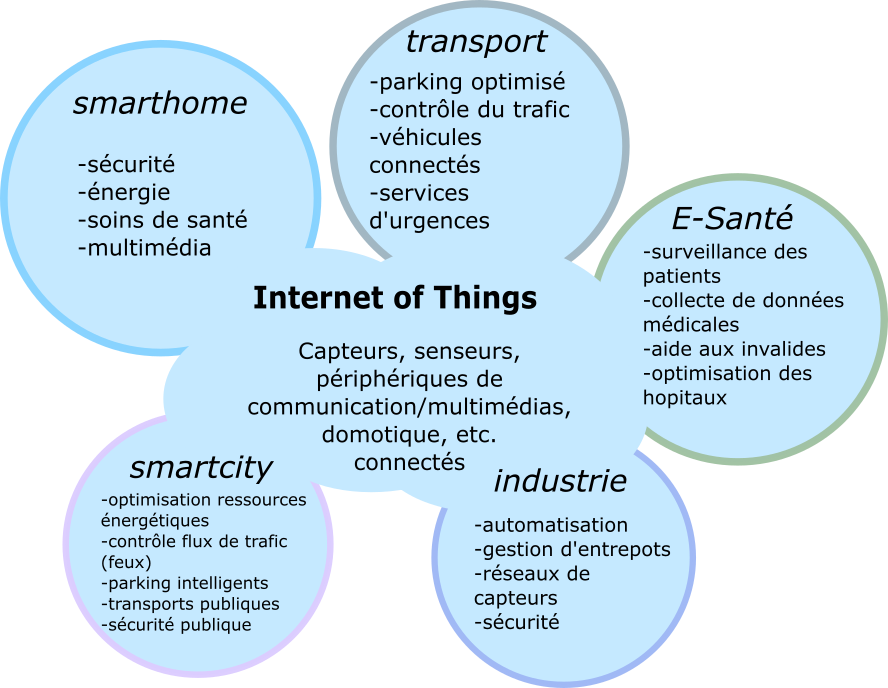
\includegraphics[width=0.65\linewidth]{IoT_domains.png}
\caption{Domaines d'application de l'IoT}
\label{domains_IoT}
\end{figure}

\newpage

\subsubsection{L'environnement \textit{smarthome}}
\label{smarthomearchi}
\par Le terme émergeant \textit{Smart Home/smarthome} est une fois de plus très englobant et général. Il n'en existe pas de définition formelle et communément acceptée. Basman M. Hasan et al. \cite{Basman2016} en présentent plusieurs. Un résultat les unifiant pourrait être
\begin{center}
 \textit{\og Une smarthome est un environnement lié au domicile particulier où plusieurs équipements ou sous-systèmes sont inter-connectés et où les informations qu'ils échangent sont collectées et utilisées afin de surveiller, réguler et automatiser l'écosystème du domicile\fg{}}.\\
\end{center}

\par L'utilisateur en tant que personne physique y vivant est donc au centre de cette architecture, et y siège comme le principal intervenant. Effectivement, l'objectif global du déploiement de tous ces dispositifs est l'amélioration de sa qualité de vie. La notion d'intelligence est intrinsèquement liée avec celle de l'interconnexion de tous ces capteurs et actuateurs déployés dans l'environnement du domicile. Il s'agit d'en récolter et regrouper toutes les données en un point central doté d'une capacité de traitement plus évoluée afin qu'il puisse en tirer une optimisation globale de l'habitation (du système de sécurité, des économies d'énergie, de temps par l'automatisation, etc.).\\

\par Une certaine classification fonctionnelle peut être établie pour distinguer de façon plus concrète les différents équipements qui peuvent intervenir dans l'écosystème d'une smarthome. Elle est schématisée par la Figure~\ref{sm_class}, inspirée de \cite{Basman2016}. Ce qui est désigné par \textit{point d'interconnexion} peut dépendre de l'architecture réelle d'une smarthome \cite{Huichen2016}. Dans la plupart des cas il s'agit d'une machine faisant office de collecteur pour toutes les données transitant dans le domicile et de gateway vers le reste de l'Internet, éventuellement le cloud associé.\\

~\\

\begin{figure}[!h]
\centering
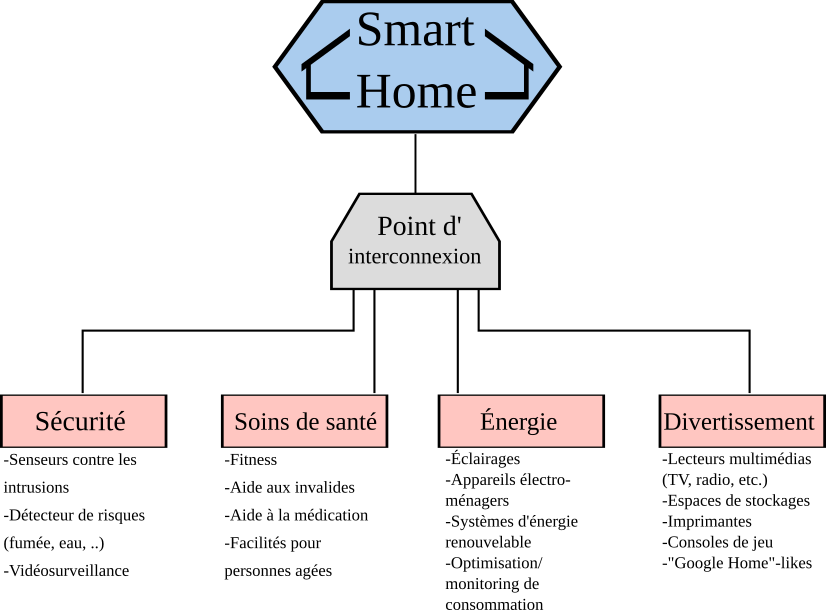
\includegraphics[scale=1.4]{smarthome_class.png}
\caption{Classification fonctionnelle des équipements \textit{IoT} d'une smarthome}
\label{sm_class}
\end{figure}

\newpage


\subsubsection{Restrictions des équipements}\label{restr_IoT}

Malgré le fait que l'ensemble des objets considérés comme appartenant à l'IoT soit très hétérogène, on peut distinguer plusieurs caractéristiques communes à beaucoup d'entre eux. Elles tendent généralement vers ce qui est vu comme une restriction par rapport à un ordinateur type classique (\textit{desktop}). Ces éléments constituent les plus gros freins au développement de la sécurité sur de tels système \cite{Wind2015}. Les conséquences de ces restrictions sont discutées plus en détail dans la \wordlink{prot_IoT}{section} de ce document.\\

\minit{Conçus pour satisfaire une unique fonction}

Le meilleur exemple est celui des capteurs. Un capteur a pour objectif de faire une mesure d'une grandeur physique (température, pression, etc.), d'en tirer une valeur numérique et de faire remonter via son interface avec le réseau cette information vers une unité centrale. Cette dernière accumule ainsi des mesures provenant des nœuds distribués pour y appliquer un traitement, et c'est à ce plus haut niveau que le processus de décision a lieu s'il est nécessaire. Ce genre d'équipement est généralement minimaliste au possible et ne peut donc pas remplir d'autre tâche.\\

\minit{Requièrent une faible consommation énergétique}

Les systèmes embarqués n'ont pas toujours accès à une source illimitée d'énergie, et auront donc une durée de vie limitée à celle de leur batterie. En conséquence, il est souhaitable d'économiser un maximum, ce qui peut se faire en réduisant les temps d'éveil de l'équipement et en optimisant le nombre d'opérations effectuées quand il tourne à plein régime. Dés lors, certains protocoles et algorithmes doivent être adaptés (relatifs aux communications réseaux mais aussi à la sécurité) \cite{Huichen2016}.\\

\minit{Sont contraints en ressources CPU, mémoire et radio}

Ces contraintes sont aussi identiques à celles des systèmes embarqués classiques. En plus de celles-ci, on peut mettre en évidence le fait que les radios (quand il s'agit d'une interface sans fil) sont assez faibles et ne permettent pas des communications à haut débit. En résulte également que des techniques comme le saut de fréquence et les algorithmes de chiffrement de type asymétrique sont plus compliquées à mettre en œuvre \cite{Leloglu2017}.\\


\minit{Sont programmés à un bas niveau d'abstraction}

Étant conçus pour ne remplir que des fonctions spécifiques, certains équipements ne sont pas programmables en utilisant des langages de haut niveau. Par conséquent, ce sont souvent des boîtes noires difficilement manipulables et statiques : les mises à jour et patch de sécurité ne sont pas déployables aisément par les constructeurs \cite{Huichen2016}. Les seules interactions que l'utilisateur lambda peut avoir avec l'équipement sont celles prévues par l'interface de ce dernier s'il y en a une (pour le configurer, consulter son état, etc.).


%\subsection{Architectures d'un système d'équipements IoT}\label{arch_IoT}

\subsection{Protocoles adaptés à l'IoT}\label{IoT_prot}

\par Les restrictions communément présentées par les équipements IoT énumérées dans la \wordlink{restr_IoT}{sous-section} imposent de repenser les protocoles utilisés dans un réseau non soumis à ces contraintes. Les protocoles décrits ci-dessous ont été conçus dans cette optique et sont utilisables dans un réseau composé d'équipements restreints en ressources, tel qu'un réseau de capteurs communiquant via la technologie sans-fil (WSN - \textit{Wireless Sensors Network}). La \wordlink{IoT_stack}{figure} en présente un récapitulatif, mettant en exergue les différences avec les protocoles utilisés dans un réseau classique (supportant la \textit{pile TCP/IP}).\\

\par Le standard \textbf{IEEE 802.15.4} a été défini par l'IEEE (Institute of Electrical and Electronics Engineers) pour les réseaux sans-fil dits \og personnels \fg \ (WPANs - \textit{Wireless Personal Area Networks}) c-à-d destinés à couvrir une zone d'émission de l'ordre de quelques dizaines de mètres. IEEE 802.15.4 supporte les couches physiques (PHY) et lien (MAC - \textit{Medium Access Control}) dans ce cadre, en considérant le manque de ressources des équipements \cite{Granjal2015} \cite{Huichen2016}.\\

\par Les réseaux utilisant IEEE 802.15.4 dans les couches plus basses sont contraints par la taille maximum que les trames peuvent contenir (pour les couches supérieures) selon ce standard, c-à-d 102 bytes. Sachant que la taille maximum d'un paquet IPv6 peut aller jusqu'à 1280 bytes par défaut, pour utiliser ce protocole il est nécessaire d'introduire un mécanisme d'adaptation. C'est l'objectif principal de la couche intermédiaire \textbf{6LoWPAN} : elle gère la fragmentation et le ré-assemblage des paquets IPv6 pour qu'ils puissent être transférés dans un réseau utilisant IEEE 802.15.4. 6LoWPAN propose d'autres services tels que la compression des en-têtes IPv6 (intuitivement nécessaire) et de l'auto-configuration de l'équipement joignant un réseau (similaire à IPv6).\\

\par L'aspect routage (sous-entendu pour des adresses IPv6) est généralement géré par le biais de \textbf{RPL} (bien qu'il soit possible de le faire avec 6LoWPAN). Il s'agit d'un protocole à vecteurs de distances adapté aux réseaux comme les WSN, comme le suggère son nom complet : \textit{Routing Protocol for Low-Power and Lossy Networks}. Il se base sur une topologie virtuelle en arbre établie par un DODAG (\textit{Destination Oriented Directed Acyclic Graph}), la racine étant un nœud qui a pour tâche de collecter toutes les informations montantes (et de les transmettre à un nœud extérieur au WSN). Plusieurs métriques peuvent être envisagées pour déterminer les routes, comme le nombre de sauts, la qualité des sources d'énergie de chaque nœud, les probabilités de réussite de transmission entre les nœuds. RPL est donc assez souple que pour s'adapter aux besoins et aux particularités des réseaux de natures variées que l'on peut retrouver dans l'IoT.\\

\par \textbf{DTLS} (\textit{Datagram Transport Layer Security}) est le mécanisme de sécurisation sur lequel peuvent se reposer les applications utilisées par les équipements IoT. Son homologue dans les réseaux non restreints est TLS, qui se repose sur la fiabilité de transport garantie par TCP : si un paquet est pas ou mal délivré, la connexion est interrompue \cite{Lakkundi2014}. DTLS est conçu pour fonctionner par dessus \textbf{UDP}, qui est le protocole \textit{de facto} utilisé pour le transport dans les réseaux IoT (celui-ci demandant moins de ressources). Il n'est pas forcément destiné à l'IoT, aussi des implémentations ont vu le jour dans cette optique (\href{https://projects.eclipse.org/proposals/tinydtls}{TinyDTLS}).\\

\par Du côté applicatif, \textbf{CoAP} est un bon candidat. Ce protocole est maintenu par l'IETF, par l'équipe du CoRE (\textit{Constrained RESTful Environments}) et est de fait basé sur l'architecture REST \cite{Granjal2015} comme son homologue HTTP. Il s'agit donc d'un modèle client-serveur. CoAP aspire à restreindre le dialecte HTTP à un sous-ensemble adapté aux contraintes des équipements IoT (aux communications 6LoWPAN) et est prévu pour fonctionner sur UDP. Ce dernier n'étant pas un protocole de transport fiable, CoAP implémente un mécanisme simple impliquant des messages \textit{Confirmables} et \textit{Acknowledge} pour pouvoir assurer un minimum de fiabilité si les données à transmettre sont critiques.\\

\par \textbf{MQTT} est un autre protocole qui diffère de CoAP sur plusieurs points\footnote{\url{https://www.eclipse.org/community/eclipse_newsletter/2014/february/article2.php}}. C'est un protocole de messagerie orienté souscription/publication léger par rapport à HTTP, la taille des messages se restreignant à quelques bytes contre plusieurs centaines \cite{Leos2014}. L'architecture est également différente : on a un équipement dit \textit{broker} qui joue le rôle de serveur de messagerie autour duquel s'articulent plusieurs clients désirant communiquer entre eux. Chaque client s'abonne à un \textit{topic} pour lequel il est intéressé en établissant une liaison avec le broker, et recevra un message concernant ce topic posté par tout autre nœud. Cette liaison, ouverte en permanence, utilise TCP et peut donc être authentifiée et chiffrée avec TLS. En plus du fait que la longueur des noms des topics peut poser problème avec la taille maximum des frames 802.15.4, cette utilisation de TCP pose problème pour les nœuds trop limités en ressources. Un port vers UDP du nom de \href{http://www.mqtt.org/new/wp-content/uploads/2009/06/MQTT-SN_spec_v1.2.pdf}{MQTT-SN} a été établi à cette fin.\\

\begin{figure}[!h]
\centering
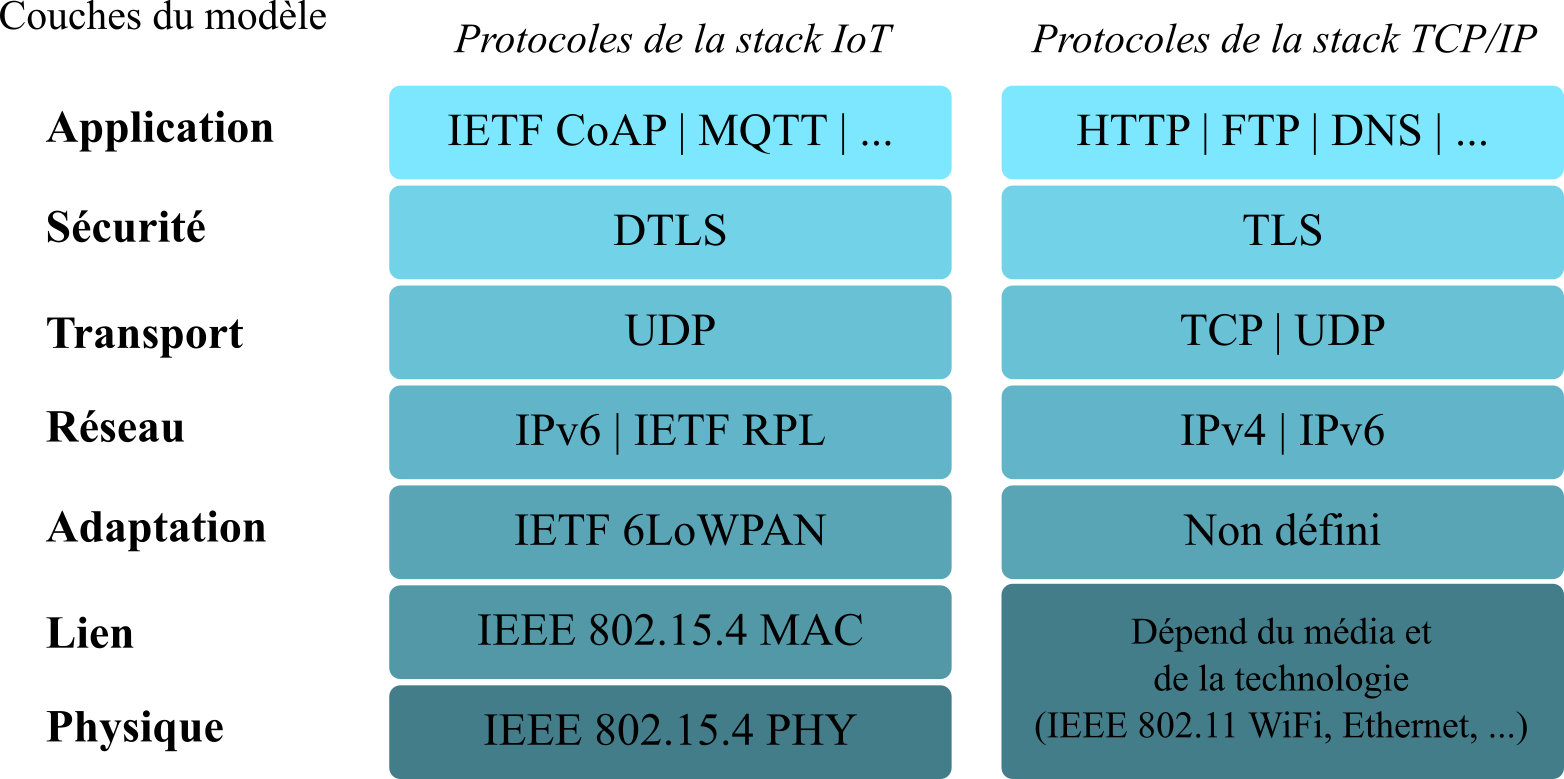
\includegraphics[scale=0.85]{IoT_stack.png}
\caption{Comparaison du modèle en couche classique (TCP/IP) avec celui adapté à l'IoT}
\label{IoT_stack}
\end{figure}

%------------- PARE FEUX -------------

\section{Présentations des pare-feux}

\subsection{Généralités}\label{gen_FW}

Un pare-feu est un dispositif, virtuel ou matériel, qui surveille et contrôle le lien entre un réseau dit de confiance et un réseau extérieur non fiable. Typiquement, ce réseau potentiellement dangereux est Internet et la zone à protéger est le réseau interne d'une entreprise ou d'une habitation. L'existence des pare-feux est une conséquence du besoin d'outils de protection aux bordures de réseaux distincts contrôlés par des entités différentes. D'une part, il faut garantir que des données internes confidentielles restent à l'intérieur du réseau de confiance. D'autre part, il est nécessaire de filtrer les données entrantes et sortantes de ce réseau de sorte qu'aucune menace ne s'y infiltre par des flux, même initiés depuis l'intérieur du réseau de confiance. Ces filtres sont créés et assemblés à partir de \textit{politiques} ou \textit{règles} définies par défaut ou par les personnes compétentes liées à l'entité gérant le réseau.

\subsection{Différentes positions et fonctions dans l'architecture réseau}

\par Deux classes de pare-feux sont distinguables en fonction de ce qu'ils visent à protéger. La première correspond aux pare-feux au niveau réseau (\hyperref[netw_fw]{\textit{network firewalls}}), situés en bordure de LANs, WANs et intranets. Ceux-ci, de par leur nature de barrière entre réseaux, peuvent également fournir des services plus évolués : système de NAT, gestion de \textit{zones démilitarisées} (définies ci-dessous), service DHCP, etc. \cite{Shimonski2013} La seconde classe agit au niveau des nœuds du réseau eux-mêmes (\hyperref[host_fw]{\textit{host-based firewalls}}), protégeant une machine physique et non pas un réseau entier. Ces pare-feux se présentent donc sous forme de logiciels, directement intégrés au niveau du système d'exploitation ou installés à un plus haut niveau.\\

\par La figure \wordlink{netw_IDS}{figure} schématise la place de ces dispositifs, mettant en scène le scénario simplifié d'un utilisateur surfant sur le site d'une entreprise. Une requête HTTP pour une page est créée et envoyée depuis le domicile, destinée aux serveurs de l'entreprise. Ceux-ci sont protégés derrière une machine dédiée uniquement à la fonction de pare-feu (qu'on qualifie alors par le terme \textit{appliance}), dans une zone tampon désignée par \textbf{DMZ} pour \textit{Demilitarized Zone} (zone démilitarisée). Cette zone intermédiaire est un sous-réseau contenant les machines étant destinées à être accédées depuis Internet mais qui n'ont aucun besoin d'accéder au réseau local de l'entreprise (typiquement des serveurs). Ainsi, si une attaque contre ces machines aboutit et que l'attaquant en prend le contrôle, il n'a pas encore un accès direct aux autres machines de l'entreprise (si le pare-feu est toujours fonctionnel). Cela permet en plus d'établir un filtrage plus fin effectué par le pare-feu, qui utilise des règles différentes en fonction de la zone ciblée et donc des services à considérer comme légitimes.

\subsubsection{Les pare-feux niveau réseau}\label{netw_fw}

\par Afin de remplir leur fonction, ces pare-feux sont placés en bordure du réseau à protéger et sont  directement liés aux machines qui font office de \textit{gateway} (routeurs). Le trafic échangé entre les réseaux ainsi connectés passe donc par le pare-feu afin d'être analysé et filtré, ce qui peut représenter beaucoup de données à traiter. Le pare-feu doit offrir une vitesse de traitement proportionnelle aux débits et à la qualité des liens qui le traversent afin de ne pas être un goulot d'étranglement. C'est pourquoi ces pare-feux doivent être très efficaces et sont communément portés (partiellement) au niveau matériel. On parle de \textit{hardware-based firewall appliances}, qui sont des machines physiques dont le seul objectif est de remplir les tâches d'un pare-feu le plus efficacement possible. On y retrouve deux composants : la partie applicative software ou firmware remplissant la fonction de pare-feu, qui repose sur la deuxième partie plus basse constituée de juste ce qu'il faut d'un OS particulier (\textit{jeOS} - \textit{just enough Operating System}). Cet OS est généralement propriétaire, lié au fabriquant du hardware sur lequel les deux parties opèrent et donc optimisé pour garantir les performances requises.\\

\par À plus petite échelle, dans un réseau domestique par exemple, on retrouve également des pare-feux directement implémentés dans le routeur qui fait office de \textit{gateway} pour l'habitation. Ceux-ci sont fatalement moins efficaces et complets que les matériels spécialement dédiés à cette unique fonction.\\

\newpage

\par À titre indicatif, la Figure~\ref{cisco_FW} donne un exemple d'une \textit{appliance} pare-feu issue de la gamme des Cisco ASA 55xx-X, la dernière génération que Cisco a introduit sur le marché en 2018 \cite{wikiASA}. Il ne s'agit pas du modèle le plus performant de la gamme en comparant les \href{https://www.cisco.com/c/en/us/products/collateral/security/asa-5500-series-next-generation-firewalls/datasheet-c78-733916.html}{performances et fonctionnalités}, mais convient typiquement bien pour être déployé dans une petite entreprise (son prix avoisine 500\euro). Dans le cas d'une habitation, l'analogue correspondant est dans la majorité des cas le modem distribué par le fournisseur d'accès internet au domicile. La société Proximus fournit par exemple des \textit{b-box}, que leurs clients peuvent configurer par une interface web. Dans ces configurations, il existe bien un onglet intitulé \textit{firewall}, mais celui-ci ne présente que peu d'options de configuration comme le montre la Figure~\ref{proxi_FW}. Dans d'autres onglets, on peut trouver d'autres fonctionnalités qui peuvent y être relatives : restriction d'accès pour certains nœuds en fonction de l'heure (par adresse MAC) et blocage de certains sites par domaine. Cela semble assez faible, les utilisateurs du réseau ont tout intérêt à installer sur leurs équipements personnels des \hyperref[host_fw]{pare-feux pour hôtes}.

% https://en.wikipedia.org/wiki/Comparison_of_firewalls
%https://www.cisco.com/c/en/us/products/security/asa-5500-series-next-generation-firewalls/data_sheet_c78-345385.html
\begin{figure}[!ht]
\centering
\begin{minipage}{.4\textwidth}
  \centering
  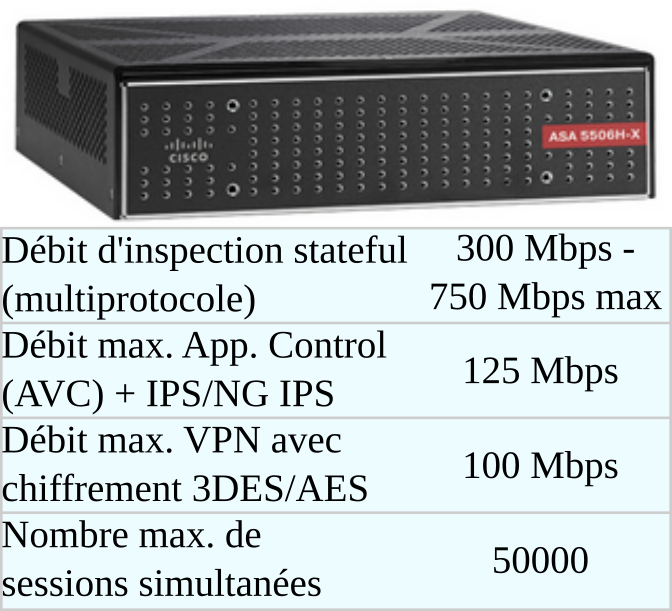
\includegraphics[width=.6\linewidth]{desc_cisco_ASA-5506H-X.png}
  \caption{Cisco ASA 5506H-X}
  \label{cisco_FW}
\end{minipage}%
\begin{minipage}{.6\textwidth}
  \centering
  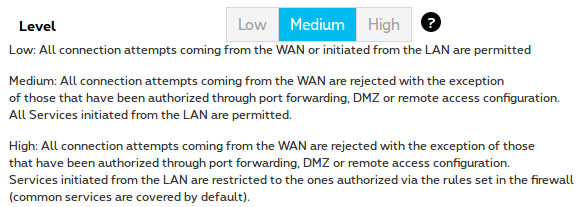
\includegraphics[width=1.0\linewidth]{proximus_FW.png}
  \caption{Options de config. du pare-feu pour une b-box 3V}
  \label{proxi_FW}
\end{minipage}
\end{figure}


\subsubsection{Les pare-feux niveau hôte}\label{host_fw}

\par Du fait que les pare-feux de cette classe sont généralement déployés sur des machines de type desktop, la dénomination \textit{pare-feu personnel} est aussi utilisée. Ces ordinateurs sont généralement munis de tels pare-feux par défaut ou peuvent tout du moins supporter leur installation par l'utilisateur si l'OS utilisé est classique (Windows, MAC OS X, ...). Le pare-feu agit jusqu'au niveau applicatif \cite{Kokko2017} et sous forme d'un \textit{service} ou d'un \textit{daemon} en fonction du système d'exploitation utilisé. Cela permet une proximité étroite avec l'OS et les autres processus. Le pare-feu personnel est donc capable de contrôler le trafic réseau demandé par chaque application et de détecter les menaces engendrées par certains flux. Ces dernières peuvent être entrantes ou sortantes : une machine extérieure qui tente d'établir une connexion suspecte ou un exécutable sur la machine à protéger qui initie un trafic avec une cible blacklistée, par exemple.\\

%https://www.itprotoday.com/security/personal-firewalls
%https://en.wikipedia.org/wiki/Personal_firewall

\par Les principales fonctionnalités d'un pare-feu personnel devraient être au minimum les suivantes \cite{Shimonski2013}
\vspace{0.1cm}
\begin{itemize}
\item[$\bullet$] Bloquer les attaques et comportements dangereux du réseau extérieur : scanning des ports ouverts, attaques par fragmentation, \textit{IP Spoofing}, etc.   
\vspace{0.2cm}
\item[$\bullet$] Stopper les menaces venant de l'intérieur : un exécutable comme un \textit{malware} ou un \textit{spyware} qui tente d'établir une connexion vers l'extérieur doit être bloqué et mis en quarantaine
\vspace{0.2cm}
\item[$\bullet$] Présenter de l'automatisation car d'une part car un utilisateur non-expérimenté pour sa configuration doit quand même rester protégé et d'autre part il doit pouvoir se mettre à jour automatiquement
\vspace{0.2cm}
\item[$\bullet$] Agir au niveau applicatif : un malware pourrait utiliser le port web 80 pour se répandre par exemple, pour détecter cela il faut analyser les payloads des paquets et disposer d'une base de données à jour pour y déceler des patterns malicieux sur base de leur signature
\vspace{0.2cm}
\item[$\bullet$] Alerter l'utilisateur quand un événement survient, et le logger avec suffisamment d'informations pour qu'il puisse prendre une décision adaptée
\vspace{0.2cm}
\item[$\bullet$] Éviter les \textit{faux-positifs} (bloquer du trafic légitime)
\end{itemize}
\vspace{0.5cm}

\newpage

\par Que ce soit en entreprise ou dans une habitation, il est donc probable que l'on retrouve des pare-feux appartenant à ces deux classes distinctes là où ils sont efficaces (voir  \wordlink{netw_IDS}{Figure}). Il ne s'agit que d'échelles différentes, qui impliquent également des intervenants différents. En entreprise, l'administrateur sécurité/réseau configure du matériel spécifique afin de sécuriser les frontières de son réseau tout en préservant ses performances. Il est aussi possible qu'il installe dans les machines internes de son réseau des pare-feux assez puissants pour empêcher les propagations des attaques déclenchées. Dans le domicile, l'habitant est sommairement protégé par le routeur fournit par son FAI qui inclut un pare-feu réseau par défaut. S'il est un minimum expérimenté, il sera à même d'installer et configurer des pare-feux personnels sur chacun de ses équipements connectés, pour autant que cela soit possible (par exemple, les contraintes liées aux équipements de l'IoT décrites dans la \wordlink{restr_IoT}{sous-section} sont un  frein à cela).   


\begin{figure}[!h]
\centering
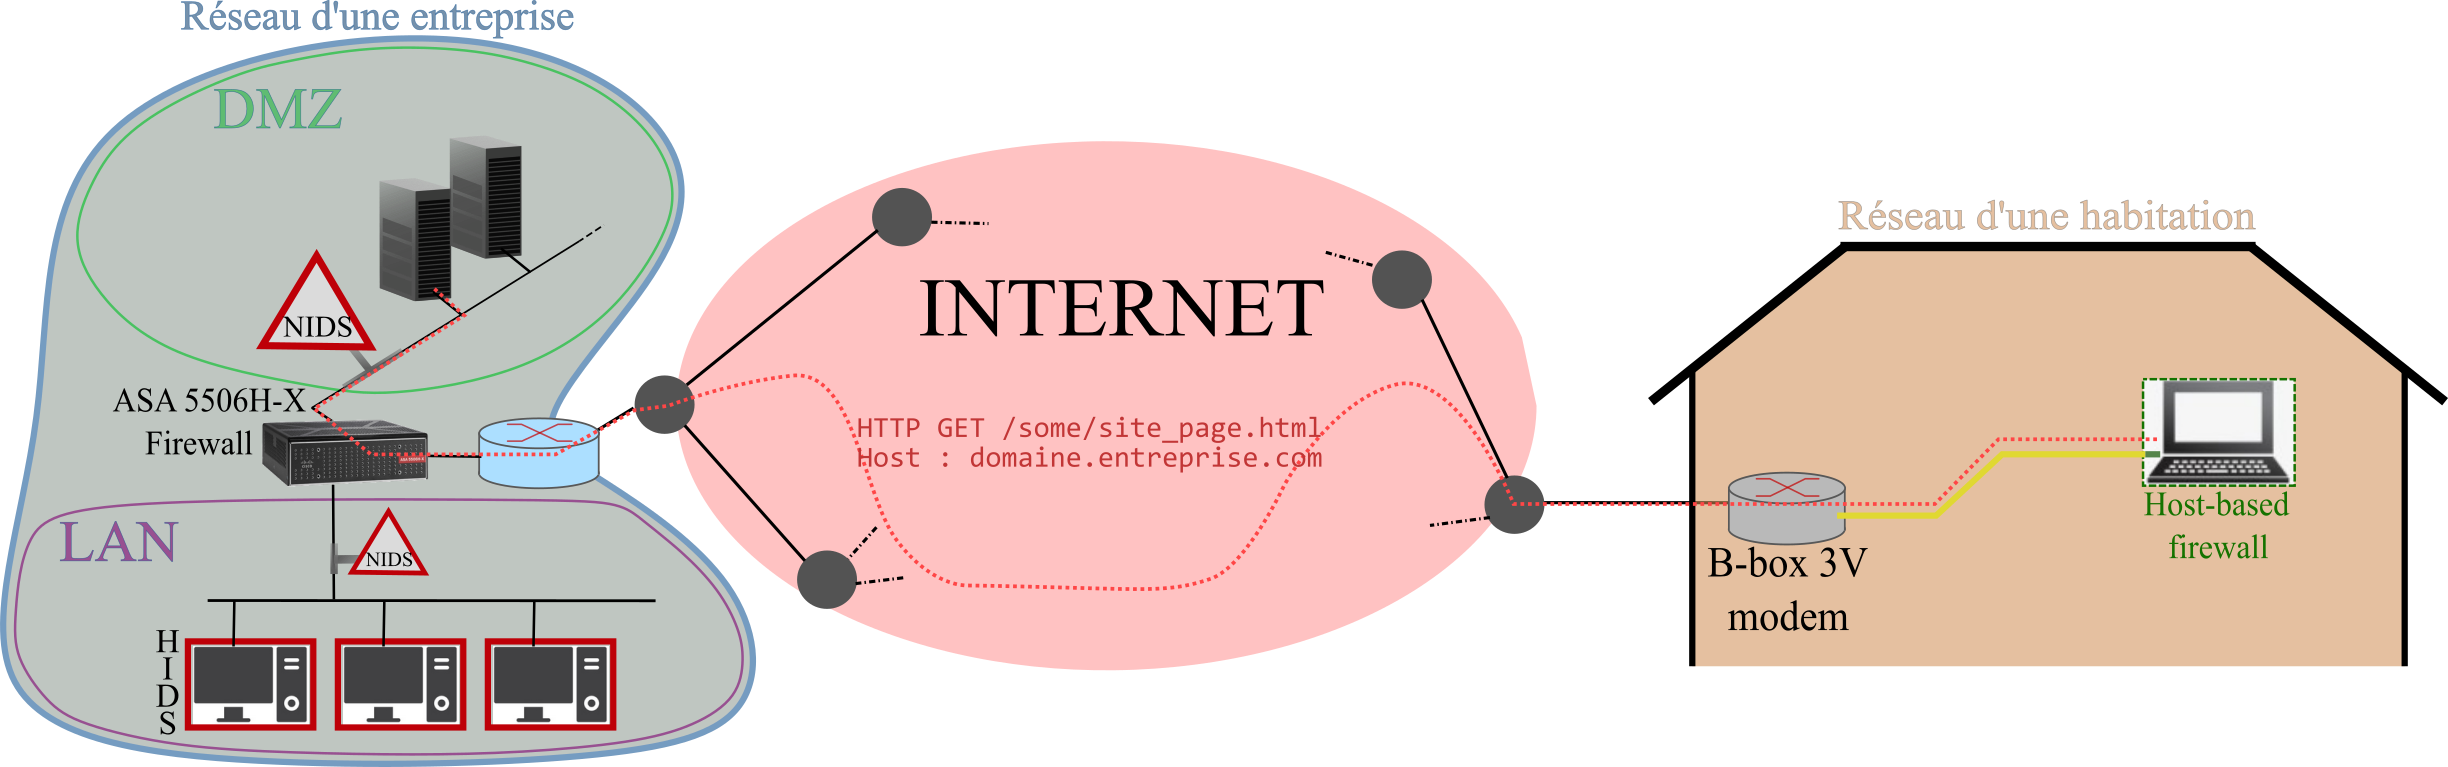
\includegraphics[scale=1.65]{netw_IDS.png}
\caption{Schéma récapitulatif des places des différents dispositifs de protection dans un réseau}
\label{netw_IDS}
\end{figure}

\subsection{Les types de pare-feu}

\subsubsection{Pare-feu de filtrage (sans état)}

Aussi désignés dans la littérature par le terme \textit{stateless}, ces pare-feux sont les plus rudimentaires, le premier prototype étant celui élaboré par Jeffery Mogul en 1989 \cite{Shieha2014}. Généralement, ces pare-feux sont rapides mais peu efficaces car facilement dupés. Un pare-feu de ce type inspecte chaque paquet individuellement et détermine s'il peut passer sur base d'un ensemble de règles écrites que ses en-têtes vérifient ou non. Ces règles portent sur les en-têtes TCP/IP (également UDP), les options y attenant et l'interface d'entrée. Plus en détail : les adresses IP source et destination, les ports source et destination au minimum seront soumis aux filtres du pare-feu. Il y a plusieurs problèmes avec cette approche :
\vspace{0.2cm}
\begin{itemize}
\item[$\bullet$] Il n'y a aucune vérification au dessus de la couche transport : la partie applicative peut contenir n'importe quoi
\vspace{0.2cm}
\item[$\bullet$] Le pare-feu n'est pas dynamique : il n'apprend rien du trafic qu'il laisse passer. Aucun état n'est retenu, alors que par exemple TCP est un protocole lié à une machine à état (orienté connexion) dont il pourrait être possible de garder une trace
\vspace{0.2cm}
\item[$\bullet$] Les règles sont très redondantes à écrire pour être efficaces, très peu modulables et facilement sujettes aux erreurs et oublis
\end{itemize}
\vspace{0.25cm}

Les paquets ICMP peuvent également faire l'objet d'un filtrage du même acabit \cite{Shimonski2013}.
Ce type de pare-feu tombe en désuétude car il est trop simple à duper par des attaquants.  


\newpage

\subsubsection{Pare-feu à état}

Le but de ce type de pare-feu dit \textit{stateful} est d'améliorer les techniques de filtrage sans état en maintenant de l'information sur les flux passant au travers, principalement TCP. Effectivement, au contraire d'UDP, TCP est un protocole qui garde un état qui se traduit dans certains champs de ses headers. Dès lors, le pare-feu peut accéder à cette information, l'analyser et l'utiliser pour en déduire dans quel état est actuellement la connexion entre les deux processus communiquant sur les deux hôtes impliqués. Cela peut se traduire par l'inspection des flags (SYN, FIN, ...), des numéros de séquences et acquittements qui permettent au pare-feu de contrôler en conséquence le contenu d'une table interne des connexions.\\ 

\par L'établissement d'une connexion TCP se fait comme suit : lors de la réception du premier paquet TCP par le pare-feu, celui-ci va le soumettre à ses règles de filtrage définies comme dans un pare-feu sans état. Si le paquet est valide, il est retransmis pour poursuivre librement sa route et une entrée est ajoutée dans la table interne du pare-feu. Celle-ci va changer d'état à chaque paquet de la communication reçu, jusqu'à arriver dans un état dit \textit{established} correspondant à la fin du 3-way handshake TCP. Tous les paquets suivants pourront alors être traités rapidement en établissant la correspondance entre ses en-têtes et celles de l'entrée en état estbalished dans la table (qui sont donc théoriquement également légitimes). Cette façon de procéder est plus efficace que de soumettre chaque paquet individuellement aux règles de filtrage qui peuvent être complexes et demander beaucoup de travail et donc gourmandes en temps.\\

\par Dans le cas d'une communication utilisant UDP, le contrôle possible est moins fin car il ne s'agit pas d'un protocole à état et les échanges ne sont pas bidirectionnels. Dans ce cas, lorsque le premier paquet d'une transmission arrive en entrée du pare-feu, il est soumis aux règles de filtrage. S'il est considéré comme correct, le pare-feu ajoute une entrée dans sa table pour les couples d'adresses et ports et considérera les suivants comme légitimes. Cette entrée expirera après un temps donné sans autre nouveau paquet la matchant. 



\subsubsection{Pare-feu applicatif}\label{appfw}

\par Ce type de pare-feu peut être considéré comme une extension complète aux simples pare-feux à états dans le but d'en améliorer la fiabilité. Là où ces derniers sont capables de déterminer quels protocoles sont utilisés et autorisés sur chaque port, les filtres ajoutés au niveau applicatif peuvent en plus déduire à quelles fins sont utilisés ces protocoles (l'inspection va jusqu'à la couche 7 du modèle OSI). Il s'agit cependant de plus que de simples filtres, c'est une technologie à part entière qui est utilisée : l'inspection profonde des paquets ou \textit{deep packet inspection} (DPI). Les pare-feux utilisant la DPI mêlent les fonctionnalités d'un pare-feu à état avec les systèmes de détection et prévention d'intrusions (sous-sections~\ref{IDS} et \ref{IPS}). La décision de bloquer ou de laisser passer le paquet tient compte de ce qu'il contient réellement au niveau données et de l'interprétation qui en est faite pour déterminer s'il représente un danger.\\

\phantomsection
\label{waf}
\par Par exemple, les \textit{Web Application Firewalls} (WAF) sont une sous-catégorie des pare-feux applicatifs qui opèrent un filtrage sur le trafic HTTP. Ils peuvent donc filtrer le trafic sur base de certaines règles d'accessibilités fixées en bloquant des requêtes aux URL douteuses ou considérées comme non éthiques vis-à-vis de l'organisme maintenant le réseau par lequel elles transitent. Outre cela, les WAFs permettent également de se protéger contre les attaques dites de type \textit{parameter tampering} (injection SQL, cross-site scripting, etc.) \cite{Palka2011}, ainsi que d'inclure des filtres anti-spam pour les courriels \cite{wikifwFR}.\\

\par Plus généralement, les pare-feux applicatifs permettent de se protéger des virus, vers et tentatives d'\textit{exploits} de faiblesses connues des systèmes à protéger \cite{wikiappfw} \cite{Palka2011}. Un autre avantage d'analyser jusqu'à la couche 7 grâce à la DPI est que certains protocoles (FTP par exemple) utilisent la couche applicative pour transmettre des informations relatives aux couches plus basses (adresses IPs, ports, etc.) et qui seront impliquées dans des communications passant par le dispositif pare-feu \cite{wikifwFR}. Comme illustré par l'exemple des WAFs, le principal défaut inhérent à leur nature réside dans le fait que pour chaque type de trafic applicatif que l'on souhaite contrôler, un travail spécifique doit être opéré (établir des règles dédiées par exemple) \cite{wikifw}. 

\newpage

\subsubsection{Pare-feu applicatif proxy}

Ces pare-feux mêlent l'inspection au niveau applicatif et le rôle de proxy pour les flux qui sont destinés à le traverser originellement. Ainsi, il devient réellement un intermédiaire entre les deux parties communiquant, interceptant les paquets pour les analyser puis les retransmettant vers le destinataire comme s'il en était la source \cite{Shimonski2013}. Avant cette retransmission, le paquet peut être inspecté du point de vue de toutes ses couches et déterminé comme étant dangereux en fonction des opérations de filtrages effectuées dans le proxy. Un contrôle très fin peut donc être opéré. Cela garantit un niveau de sécurité plus haut que les pare-feux de filtrage pur qui traitent les paquets à la volée \cite{frameIP}.\\

\par Cette approche possède cependant trois gros désavantages : 
\begin{itemize}
\vspace{0.2cm}
\item[$\bullet$] Clairement, l'impact sur les performances du réseau n'est pas insignifiant (surtout si le pare-feu n'est basé que sur du software pur et pas sur une machine adaptée)
\vspace{0.2cm}
\item[$\bullet$] À chaque nouveau protocole applicatif que l'on souhaite pouvoir filtrer de la sorte, un nouveau dispositif proxy correspondant doit être pensé et développé pour en inspecter le trafic
\vspace{0.2cm}
\item[$\bullet$] Si un proxy présente une faille de sécurité, un assaillant peut l'utiliser comme un vecteur d'attaque et prendre le contrôle du système sur lequel il tourne. S'il parvient alors à désactiver les services relatifs au pare-feu, la voie vers ce qu'on souhaitait protéger se retrouve toute ouverte
\end{itemize}


\subsubsection{Pare-feu identifiant}\label{idfw}

Pour ce type de dispositif, on veut pouvoir définir des règles de filtrage en fonction de l'utilisateur ou le groupe qui se cache derrière un paquet ou un flux. Plusieurs schémas d'association existent, définissant ce à quoi la notion d'un utilisateur correspond. Par exemple certains de ces pare-feux comme \href{http://www.openbsd.org/faq/pf/authpf.html}{authpf}\footnote{\url{http://www.openbsd.org/faq/pf/authpf.html}} sous OpenBSD, qui étant placés sur un gateway, exigent qu'avant d'autoriser un flux l'utilisateur d'un hôte communiquant doit établir une connexion SSH avec ce dernier. Un autre type d'association possible peut se faire par adresse MAC.\\

\par Les pare-feux destinés aux entreprises développés par Cisco (ASA) \cite{cisco2018} et Palo Alto Networks \cite{Kokko2017} utilisent des gestionnaires d'annuaires d'utilisateurs basés sur les services \href{https://fr.wikipedia.org/wiki/Active_Directory}{Windows Active Directory}. Dans ces bases de données utilisateurs, on retrouve les différentes adresses IP associées à un utilisateur particulier ainsi que les groupes qu'ils composent. Les interactions avec le pare-feu sont transparentes à ce niveau, en effet ce dernier travaille avec les objets \og utilisateurs \fg et non plus directement les IPs (bien que cela reste possible). Procéder de cette façon apporte plusieurs avantages \cite{cisco2018}:
\vspace{0.2cm}
\begin{itemize}
\item[$\bullet$] Cela simplifie la création et la gestion des politiques de sécurité du pare-feu
\vspace{0.2cm}
\item[$\bullet$] Offre la possibilité d'identifier facilement les utilisateurs utilisant le réseau
\vspace{0.2cm}
\item[$\bullet$] Simplifie la surveillance des activités des utilisateurs du réseau et permet d'identifier la source de menaces
\end{itemize} 

\newpage

%https://www.frameip.com/firewall/
\subsection{Systèmes de détection d'intrusion (\textit{IDS})}\label{IDS}
%https://www.ibm.com/developerworks/library/se-intrusion/index.html
%https://www.comparitech.com/net-admin/network-intrusion-detection-tools/
Ce type de systèmes, abrégé par IDS pour \textit{intrusion detection system}, est analogue à ce qu'est un système d'alarme intérieur dans l'environnement d'une habitation : quand les dispositifs de protection mis en place à l'entrée sont contournés (une présence non permise est détectée à l'intérieur), l'alarme est lancée et des actions sont éventuellement prises en conséquence. Les IDSs sont donc des sentinelles qui surveillent le réseau interne, logiquement placées après le pare-feu dans le sens entrant. Ces systèmes se présentent sous la forme d'outils spécialisés dans l’interprétation des logs des routeurs, pare-feux, serveurs et autres agents du réseau interne. Les IDSs sont épaulés par une base de données des signatures d'attaques déjà connues et y comparent le contenu des logs afin de trouver des \textit{patterns} qui correspondent \cite{Shimonski2013}. Dans une telle situation, plusieurs actions allant de simplement alerter l'administrateur réseau à couper les accès réseaux des machines peuvent être déclenchées, en fonction du degré de certitude (correspondance forte entre les signatures) et de la menace.\\

\par Tout comme les pare-feux, les IDSs peuvent être des ressources software ou reposer sur du hardware spécifique. Dans le cas ou il s'agit de software, ils sont établis sur la même machine que le pare-feu, les proxy ou autres dispositifs de bordure de réseau. S'ils se présentent sous forme d'équipements hardwares spécifiques, ils sont installés de sorte à contrôler et surveiller de près un de ces dispositifs sensibles. Le trafic tant entrant que sortant peut être analysé par les IDSs, car les attaques peuvent autant venir de l'extérieur que se déployer depuis l'intérieur (chevaux de Troie, spywares, etc.).\\

\par L'analyse des événements repose communément sur deux techniques. La première, la détection par signature (\textit{signature detection}), utilise une base de données de signatures d'attaques déjà connues et se base sur le trafic et les patterns observés pour établir un match avec ces signatures. La seconde approche est celle de la détection d'anomalies (\textit{anomaly detection}). Il est question d'utiliser des heuristiques afin de distinguer les situations et comportements anormaux, sur base de profils types construits par analyses statistiques, agencements de règles ou réseaux neuronaux. Outre la technique utilisée, trois catégories d'IDSs existent en fonction de leur place dans l'architecture réseau (leur mode de fonctionnement diffère en conséquence) :
\vspace{0.3cm}
\begin{itemize}
\item[$\bullet$] Surveillance du réseau (\textit{NIDS}:\textit{ Network-based IDS})
\item[$\bullet$] Surveillance des systèmes du réseau (\textit{HIDS}:\textit{ Host-based IDS}) 
\item[$\bullet$] Surveillance distribuée du réseau (\textit{NIDS}:\textit{ Distributed IDS}) 
\end{itemize} 

\subsubsection{Les NIDSs}

\par Ces dispositifs surveillent le réseau ou un segment de ce réseau, sous forme d'un équipement intermédiaire de capture (ses interfaces sont en mode écoute pour l'entièreté du trafic transitant par le segment). Il est important d'avoir plusieurs unités de surveillance distinctes dans le cas où le réseau est scindé en plusieurs modules/zones. Par exemple, un serveur web d'une entreprise pourrait être infecté et servir de plateforme de lancement d'une attaque depuis le réseau interne, vers un autre module contenant des serveurs internes.\\

\par Deux manières de procéder à l'analyse sont possibles : soit en mode \textit{in-line} soit en mode \textit{off-line}. Le cas de la capture du trafic par interface décrit ci-dessus correspond au mode in-line. Le trafic est analysé en temps réel, ce qui permet une plus grande réactivité mais peut constituer un goulot d'étranglement si le processus de décision est coûteux. Le mode off-line est donc plus avantageux à ce niveau, puisque le processus d'analyse et décision est opéré sur des données stockées et non pas à traiter à la volée. Une inspection plus fine est alors envisageable, cependant le principal défaut de ce mode de fonctionnement reste le manque de réactivité à une attaque.

\newpage
\subsubsection{Les HIDSs}

\par Les IDSs orientés systèmes, \textit{Host-based IDS}, sont élaborés dans le but de protéger uniquement l'hôte sur lequel ils sont déployés et non plus un segment du réseau. Ils ciblent également de façon précise le trafic qu'ils doivent surveiller en fonction de la nature du système. Par exemple, si l'hôte ne maintient aucun service DNS, il est inutile d'analyser des requêtes DNS qui lui parviendraient pour y déceler une menace exploitant une faille connue dans le protocole DNS. Puisque les HIDSs vont s'exécuter sous forme d'un processus (\textit{daemon}) sur la machine hôte qui elle-même fonctionne sous un OS classique, un lien doit être établi entre les deux pour que l'HIDS puisse surveiller le système et les interfaces réseaux. Certains vont même jusqu'à rechercher les intrusions dans le noyau de l'OS.\\

\par D'une part, un HIDS peut surveiller le comportement du système  dynamiquement en récupérant des informations que ce dernier met à sa disposition à la manière d'un antivirus. Différents indicateurs sont à interpréter :
\vspace{0.2cm}
\begin{itemize}
\item[$\bullet$] Activité de la machine même : processus qui y vivent, ressources qu'ils consomment (CPU, RAM, réseau etc.), modification dans les comptes utilisateurs
\vspace{0.2cm}
\item[$\bullet$] Activité des utilisateurs : commandes entrées, programmes lancés, tentatives d'accès à des ressources non autorisées, passage au compte administrateur
\vspace{0.2cm}
\item[$\bullet$] Patterns d'exécution ou de procédure de déploiement des vers, virus, chevaux de Troie (shell ouvert simultanément à l'ouverture d'un fichier, accès anormaux aux interfaces réseau, ...)
\end{itemize}
\vspace{0.4cm}
\par D'autre part, certaines sections plus critiques du système peuvent être intéressantes à analyser finement, car c'est généralement là qu'un attaquant voulant prendre le contrôle de la machine va laisser des traces en y installant ses outils softwares. Un HIDS voulant s'assurer que des sections critiques (système de fichiers, registres, ...) ne sont pas infectées va maintenir une base de données de leur évolution dans le temps, sous forme d'attributs et sommes de contrôles (\textit{checksums}). Ces dernières permettent d'assurer l'intégrité des ressources concernées en en comparant les valeurs régulièrement dans le temps, et notifiant les différences observées.

~\\
\subsubsection{Les DIDSs}
%https://www.symantec.com/connect/articles/introduction-distributed-intrusion-detection-systems
\par Les DIDSs se présentent sous la forme d'une architecture distribuée d'IDSs (surveillant des segments de réseaux et/ou hôtes), et d'une unité centrale de management qui récolte toutes les informations de ces dispositifs déployés. Ainsi, la machine centrale peut maintenir une vaste base de données centralisée, représentant l'état global du réseau à protéger. Cette approche présente plusieurs 
avantages :
\vspace{0.2cm}
\begin{itemize}
\item[$\bullet$] moins de faux positifs car plus de données pour justifier une prise de décision (agrégation des événements et attaques)
\vspace{0.2cm}
\item[$\bullet$] mises à jour et distribution de la base de données des signatures aisées
\vspace{0.2cm}
\item[$\bullet$] centralisation des alertes/logs, contrôle global avec une vue d'ensemble
\vspace{0.2cm}
\item[$\bullet$] réponses aux événements plus efficaces, IDSs plus simples à administrer en conséquence (ajout de nouvelles règles suite à des brèches découvertes, blacklisting d'IPs, etc.)
\end{itemize}
\vspace{0.4cm}

\par Afin de transmettre les alertes générées jusqu'à l'unité centrale efficacement, les différents nœuds IDSs du réseau devraient communiquer de façon homogène. À cette fin, un standard a été écrit sous le nom de format IDMEF (\textit{Intrusion Detection Message Exchange Format}, RFC 4765). Ce langage d'alertes est lisible par l'humain, utilisant le format XML. Utilisé par tous les nœuds qui effectuent la tâche de détection d'intrusion (quelque soit le type et l'implémentation), l'unité centrale qui récolte toutes les alertes peut utiliser un outil de pilotage de la sécurité du réseau global comme \href{https://fr.wikipedia.org/wiki/Prelude_SIEM}{Prelude}\footnote{\url{https://en.wikipedia.org/wiki/Prelude_SIEM_(Intrusion_Detection_System)}}. Cet outil normalise, trie, agrège, corrèle et en tire les conclusions sur des décisions à prendre pour protéger le réseau, tout en fournissant une interface (et des logs) via laquelle l'administrateur peut surveiller ce qui se passe globalement.

\newpage
\subsection{Systèmes de prévention d'intrusion (\textit{IPS})}\label{IPS}
%https://fr.wikipedia.org/wiki/Syst%C3%A8mes_de_d%C3%A9tection_et_de_pr%C3%A9vention_d%27intrusions_dans_les_syst%C3%A8mes_distribu%C3%A9s
\par Dans la section précédente, il était question de détection des attaques et pour certaines d'entre elles des actions à effectuer en contre-mesure pour bloquer la menace. Cela relève du domaine d'application des systèmes de prévention d'intrusion, aussi abrégé IPS pour \textit{intrusion prevention systems}. Tout comme pour les IDSs, deux types d'IPS peuvent être distingués en fonction de leur place dans l'architecture réseau : les \textit{host-based IPS} agissent au niveau local pour un hôte, tandis que les \textit{network-based IPS} défendent un réseau ou un de ses segments internes. De fait, IDSs et IPSs vont de paire puisque les contre-mesures prises par un dispositif IPS sont basées sur ce que l'IDS détecte et lui transmet comme information.
\vspace{0.2cm}
%https://community.spiceworks.com/topic/362007-how-intrusion-prevention-systems-ips-work-in-firewall
\par En plus de lancer une alerte à destination d'un administrateur et écrire des logs complets,  les actions qu'un IPS peut effectuer suite à la détection d'une menace sont généralement les suivantes :
\vspace{0.2cm}
\begin{itemize}
\item[$\bullet$] Jeter les paquets détectés comme contribuant à cette attaque
\vspace{0.2cm}
\item[$\bullet$] Bloquer tout trafic issu de la même adresse IP/du même utilisateur que celui considéré comme attaquant (mettre fin à la connexion TCP impliquée)
\vspace{0.2cm}
\item[$\bullet$] Reconfigurer le pare-feu associé pour qu'il puisse à l'avenir bloquer le trafic relatif à cette attaque
\vspace{0.2cm}
\item[$\bullet$] Si l'IPS est lié à un dispositif faisant du proxy, il peut agir sur le contenu des paquets pour neutraliser la menace (par exemple ôter un fichier infecté joint à un mail)
\end{itemize}


\subsection{Les pare-feux nouvelle génération}

Abrégés par NGFW (\textit{next-generation firewalls}), ces pare-feux font suite à ce qu'on distingue comme la troisième génération dans l'évolution des dispositifs pare-feux \cite{wikifw}, c'est-à-dire ceux qui appliquent les concepts de filtrage au niveau applicatif décrits dans la \hyperref[appfw]{sous-section~\ref{appfw}}. Les NGFW effectuent une analyse plus fine que ces derniers en utilisant les technologies avancées de \href{https://en.wikipedia.org/wiki/Deep\_packet\_inspection}{\textit{deep packet inspection}}. Les services qu'offrent la nouvelle génération de pare-feux s'étendent encore au-delà de la simple fonctionnalité d'inspection des paquets, et sont devenus des systèmes très complexes implémentant d'autres dispositifs liés à la sécurité dont les suivants :
\vspace{0.2cm}
\begin{itemize}
\item[$\bullet$] Support des technologies de (dé)chiffrement utilisées classiquement dans les réseaux
\vspace{0.2cm}
\item[$\bullet$] Les systèmes de management et contrôle sur base des identités des utilisateurs inspirés des \hyperref[idfw]{pare-feux identifiants} 
\vspace{0.2cm}
\item[$\bullet$] Les pare-feux destinés aux flux web (\hyperref[waf]{WAFs}), le filtrage d'URLs selon des politiques de sécurité et éthique
\vspace{0.2cm}
\item[$\bullet$] Des moyens de contre-mesures aux attaques empruntés aux \hyperref[IPS]{IPSs}
\vspace{0.2cm}
\item[$\bullet$] Les environnements virtuels (\textit{sandboxing}) de tests pour déceler dans un flux suspect une attaque non reconnue \cite{Kokko2017}
\vspace{0.2cm}
\item[$\bullet$] De vastes bases de données sur le cloud interrogées efficacement via un service spécialisé fourni avec le pare-feu (environnement \href{https://www.paloaltonetworks.com/documentation/80/wildfire/wf\_admin/wildfire-overview/wildfire-deployments/wildfire-global-cloud}{WildFire} et similaires)
\end{itemize}

\newpage
\subsection{Les pare-feux de référence}

\subsubsection{Sous forme de software}

\par Ces pare-feux sont destinés à être installés et utilisés par-dessus des systèmes d'exploitation génériques tels que Windows, distributions Linux et BSD, etc. En plus de protéger la machine sur laquelle ils opèrent des menaces extérieures, certains d'entre eux intègrent d'autres fonctionnalités telles que du \textit{traffic shaping} ou la gestion d'un système de NAT.\\

\minit{Windows}

\par \textbf{Windows Firewall} est intégré par défaut avec les versions de l'OS Windows postérieures à \textit{Windows XP}. Il s'agit d'un pare-feu qui se veut \og user-friendly \fg : par défaut il présente une liste de profils pré-configurés pour que l'utilisateur puisse sélectionner celui qui convient le plus à ses besoins (\textit{Public}, \textit{Private} et \textit{Domain}). Il agit comme un pare-feu à état basique mais assez complet dans sa fonction restreinte cependant, en plus d'être simple à utiliser et de disposer d'une interface graphique. Le fait qu'il soit directement incorporé dans le système permet un contrôle fin de quelles applications sont autorisées pour quels types de trafics.\\

\minit{Linux}

\par \textbf{Netfilter} est la solution de base de filtrage de paquets inclue dans le noyau Linux. Plusieurs modules liés au noyau sont également fournis pour servir d'intermédiaire dans la configuration de Netfliter, notamment sous la forme de tables de règles en chaines à appliquer séquentiellement sur les entrées à filtrer. Ces modules sont accessibles depuis l'utilitaire \textit{iptables}, sous les noms de ip\_tables, ip6\_tables, etc.\\

\par \textbf{nftables} a pour objectif de remplacer Netfilter à terme car il est sensé apporter plus de performances principalement. L'utilitaire permettant de faire le lien avec cette nouvelle solution implémentée dans le noyau est réduit à \textit{nft} (réduction du nombre de module par rapport à Netfilter).\\

\par \textbf{Shorewall} repose sur Netfilter, faisant office de couche d'abstraction pour faciliter la configuration des règles qui est assez laborieuse avec les outils comme iptables. Il permet l'écriture des règles alimentant les tables par un mécanisme de fichiers de configuration. C'est un software complet, il propose des fonctionnalités classiques telles que du NAT, du \textit{traffic shaping}, un support VPN et \href{http://www.shorewall.net/shorewall_features.htm}{autres}. Une autre fonctionnalité notable est la possibilité de partitionner le réseau en zones distinctes (ou pouvant se recouvrir l'une l'autre), permettant le contrôle de toutes les connexions entre chaque paire de zone à considérer. Cela permet notamment l'établissement aisé de zones démilitarisées (DMZ).\\ 

\minit{BSD}  

\par \textbf{Packet Filter} (pf) est comparable à Netfilter pour les noyaux Linux. C'est une solution de filtrage de paquets à état, incluant d'autres fonctionnalités classiques telles que la gestion de NAT, des mécanismes liés à la \textit{qualité de service} (QoS), une gestion des logs avancée en offrant leur configuration règle par règle. D'autres utilitaires sont venus s'y greffer, tel que \href{https://www.openbsd.org/faq/pf/authpf.html}{\textit{authpf}} qui permet un système de gateway authentifié (voir \hyperref[idfw]{les pare-feux identifiants}). Packet Filter a fait l'objet de port vers de nombreux autres systèmes d'exploitation, notamment Apple Mac OS X et iOS, NetBSD et Solaris.

\newpage

\subsubsection{Sous forme d'appliance}

Le terme \textit{appliance} désigne un appareil/système constitué du strict minimum de composants pour remplir au mieux une fonction spécifique. Du point de vue des dispositifs pare-feux, on peut distinguer trois catégories d'appliances :
\begin{itemize}
\vspace{0.2cm}
\item[$\bullet$] les pare-feux destinés aux systèmes embarqués, particulièrement contraints en ressources comme c'est le cas pour certains équipements de l'IoT.  
\vspace{0.2cm}
\item[$\bullet$] les pare-feux logiciels destinés à fonctionner au dessus d'une couche d'abstraction du hardware spécifique (ou même sur une machine virtuelle), basés sur un noyau d'OS qui est transparent à l'utilisation
\vspace{0.2cm}
\item[$\bullet$] les pare-feux reposant sur du hardware (machines dédiées vendues telles quelles) et qui utilisent le matériel et les équipements spécifiques construits à cette fin apportant de meilleures performances
\end{itemize}
\vspace{0.2cm}

\par Généralement, il s'agit de solutions destinées aux entreprises de par leur prix et leur nature. Effectivement, comme ce sont des équipements/dispositifs dédiés (presque) uniquement à la fonction de pare-feu (et à la sécurisation du réseau en général), ils sont souvent déployés comme des \hyperref[netw_fw]{pare-feux niveau réseau}. À noter que beaucoup de ces pare-feux tournent sur un OS propriétaire de l'entreprise qui les fabrique (Cisco, Check Point, etc.). Cela permet aux fabricants d'optimiser leurs produits tant au niveau performance que sécurité, restreignant leur OS au strict nécessaire (certains d'entre eux sont basés sur des noyaux déjà existants).\\

\minit{Appliances sur systèmes embarqués}

\par \textbf{IPFire} est dérivé du noyau Linux et est capable de remplir les toutes les fonctions basiques d'un routeur utilisé en conjugaison avec un pare-feu, sous des contraintes de ressource de 1GHz pour le CPU, 1GB de RAM et 4GB d'espace disque. De fait, IPFire peut être utilisé sur des systèmes comme une carte Raspberry PI ou dans des environnements virtuels. IPFire est modulable avec des \href{https://wiki.ipfire.org/addons/start}{add-ons} gérés par un utilitaire de management, \textit{Pakfire}. Cependant, \href{https://www.ipfire.org/features}{la version minimaliste} supporte déjà des fonctionnalités telles que l'inspection des paquets à état, le proxying, la prévention d'intrusions, la segmentation en zones du réseau, la gestion de QoS, les services DHCP et DNS, etc.\\

\par \textbf{IPCop} est un pare-feu open-source assez minimaliste utilisant Netfilter en arrière-plan. Les pré-requis pour le faire tourner sont : 200MHz de fréquence CPU, 64 Mo de RAM et 800 Mo d'espace de stockage. Même avec cette configuration minimale, il assure les fonctionnalités de proxy et d'IPS en plus du filtrage à état classique. Des modules peuvent être ajoutés en fonction des services supplémentaires requis : services DHCP ou DNS, \textit{trafic shaping}, liste d'accès utilisateurs, etc. IPCop est une branche divergente du projet \href{https://www.smoothwall.com/}{SmoothWall}, ce dernier s'étant développé de telle sorte qu'il n'est plus associable à un pare-feu \textit{embarqué} en plus d'être passé en partie sous licence commerciale.\\

\minit{Appliances orientées software non spécifiques aux équipements restreints}

\par \textbf{pfSense} se repose sur FreeBSD (bien qu'aucune connaissance sur ce dernier ne soit requise, puisque pfSense est une appliance à utiliser tel quel). Le software peut être installé sur une machine physique dédiée ou dans un environnement virtuel. Il est complètement open-source, et \href{https://www.pfsense.org/getting-started/}{a la prétention} d'offrir tous les services que les grandes distributions incluent dans leur appliances physiques en un seul software, gratuit et extensible. pfSense opère comme un routeur et pare-feu sur la machine dédiée, ces services étant alors configurables et mis à jour via une interface web.\\

%https://www.fortinet.com/demand/gated/gartner-magic-quadrant-utm-2018.html

\par \textbf{Untangle} est quant à lui basé sur le noyau Linux. Il est également déployable sur une machine simple dédiée ou virtuelle. Ses \href{https://www.untangle.com/shop/ng-firewall-complete/}{fonctionnalités} incluent entre autres les classiques d'un pare-feu nouvelle génération (filtrage du contenu, IPS, identification utilisateur, etc.) mais aussi la possibilité de faire du cache web, du \textit{load balancing} et du routage. Cependant, seule une version légère du software est distribuée gratuitement.\\

\newpage

\minit{Softwares reposant sur des appliances hardware}

%https://community.checkpoint.com/thread/8111-just-to-be-sure-checkpoint-is-just-a-software-based-firewall-right-do-we-have-checkpoint-hardware-firewall-just-like-cisco-asa
\par \textbf{CheckPoint Software} est une entreprise qui vend des machines dédiées à la protection des réseaux ainsi que les solutions logicielles qui les accompagnent. Le software \textit{GAiA} fait office d'OS pour les \href{https://www.checkpoint.com/downloads/products/check-point-appliances-brochure.pdf}{appliances hardwares vendues par CheckPoint} pour lesquels il est optimisé, mais peut également être déployé sur une appliance virtuelle compatible hébergée sur une \href{https://www.checkpoint.com/support-services/hcl/}{machine qui en est capable}.\\

\par \textbf{Cisco} offre des services similaires avec ses pare-feux nouvelle génération ASA 5500-X. Le software Cisco \textit{Adaptative Security Appliance} est l'OS dédié principalement aux machines de la famille ASA (encore une fois des solutions de virtualisation existent). La sur-couche \textit{Cisco Firepower Threat Defence} (FTD) est un software intégrant les fonctionnalités d'ASA et des services axés IDS/IPS nouvelle génération de \href{https://en.wikipedia.org/wiki/Sourcefire}{FirePOWER}.\\

\par Ces solutions sont généralement utilisées dans des réseaux de grande taille, donc en entreprise. Les appliances hardwares sont vendues telles quelles à prix élevé, et le software fourni avec y est intégré pour en garantir les performances, tant au niveau des débits que de la détection et du blocage des menaces. Cependant, il n'est pas vain de s'y intéresser car certaines technologies sur lesquelles elles sont basées sont parfois réutilisables à plus petite échelle (dans le cadre de solutions pour protéger un réseau domestique entre autres). Par exemple, FirePOWER a été développé à partir du software open-source \href{https://en.wikipedia.org/wiki/Snort_(software)}{Snort} et utilise les bases de données de définitions de signatures virales issues d'un utilitaire anti-virus nommé \href{http://www.clamwin.com/content/view/58/27/}{ClamWin}, libre également.

\newpage

%------------- SECU IoT -------------

\section{La sécurité dans l'IoT}\label{prot_IoT}

\subsection{Motivations et exemples}\label{motiv_IoT}

À priori, dans le cadre d'une smarthome, les équipements relevant de l'IoT sont plutôt des petits accessoires, voire gadgets (montres, lampes, balances connectées par exemple). On pourrait donc se dire qu'introduire des mécanismes de sécurité avancés dans de tels petits systèmes n'est pas primordial, l'aspect fonctionnel étant plus mis à l'honneur. C'est d'ailleurs ce qu'ont fait beaucoup de constructeurs, mettant sur le marché des équipements possédant des failles de sécurité importantes ou des faiblesses au niveau du design de conception. Un exemple interpellant est le fait que pour un équipement qui possède une interface accessible par un portail de sécurité par identification (requérant une entrée  de la forme \textit{user/password}), les valeurs d'usine par défaut sont laissées telles quelles, l'utilisateur n'étant jamais invité à les modifier \cite{Leos2014}. Ainsi, il existe des listes établies de ces identifiants par défaut en fonction du constructeur (\href{https://www.ispyconnect.com/userguide-default-passwords.aspx}{pour les webcams} par exemple) qui, combinées avec des outils puissants comme \href{https://www.shodan.io/}{Shodan} ou \href{https://censys.io/}{Censys}, constituent des brèches dans la protection de l'habitation pour les attaquants qui savent les exploiter. La \wordlink{shodans}{Figure} illustre la déconcertante facilité avec laquelle il est possible d'attenter à la vie privée des utilisateurs inconscients (une unique requête a été nécessaire).\\


    \begin{figure}[!h]
       \noindent\makebox[\textwidth]{%
       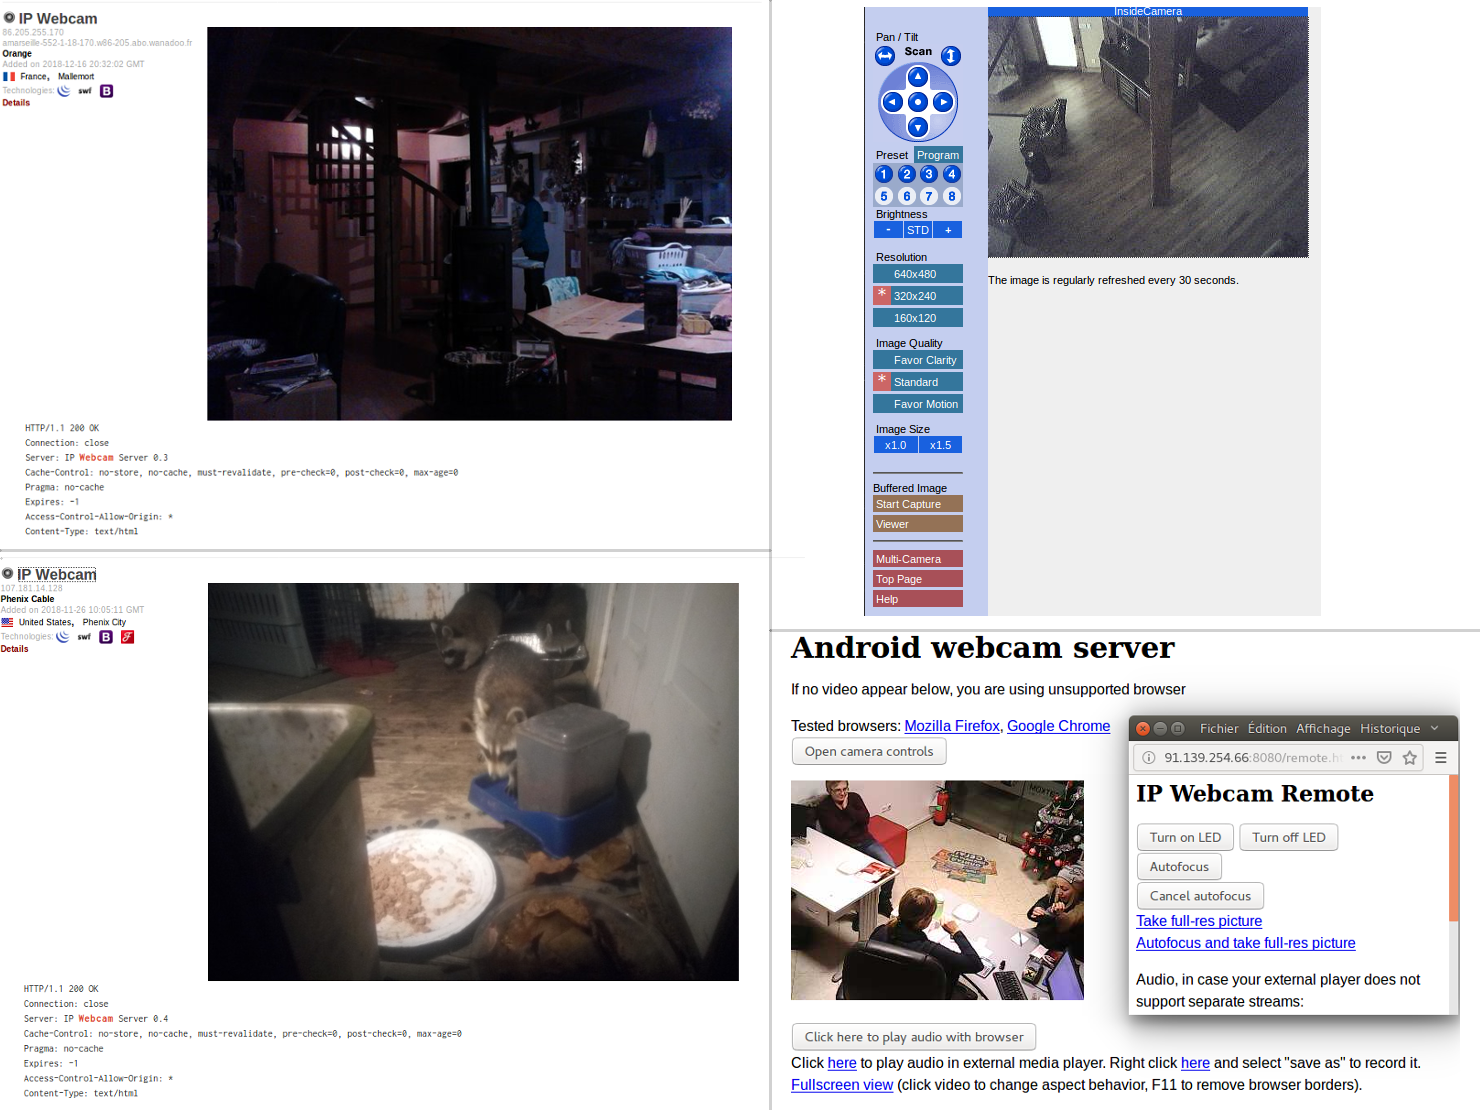
\includegraphics[width=1.1\textwidth]{Shodans.png}}
       \caption{Résultats d'une brève recherche avec Shodan ciblant des caméras en réseau non ou peu protégées}
       \label{shodans}
    \end{figure}

\newpage

\par Évidemment, l'utilisateur \og final \fg \ n'est pas le seul qui puisse en subir les conséquences. Ses équipements peuvent entre autres rejoindre un ensemble d'autres  objets connectés infectés, reconfigurés malicieusement en vue d'effectuer une attaque de masse de type \textit{DDOS} sur une cible étrangère au réseau domestique. C'est ce qui s'est passé avec \href{https://en.wikipedia.org/wiki/Mirai_(malware)}{\textit{Mirai}} \cite{wikiMirai}, un malware catégorisé comme \textit{botnet} décelé bien après son expansion et qui a été utilisé dans plusieurs attaques menées sur le fournisseur de services DNS \textit{Dyn}, la société d'hébergement \textit{OVH} et bien d'autres. Mirai n'est pas un cas isolé, et les hackers ont pleinement saisi l'opportunité qu'incarne l'IoT : il existe beaucoup de failles connues et exploitables sur des équipements hétérogènes, et celles-ci sont en partie rendues publiques sur par exemple des \href{https://github.com/nebgnahz/awesome-iot-hacks}{dépôts githubs} et des \href{https://hackforums.net/forumdisplay.php?fid=193}{forums dédiés}.\\

\par Les équipements qu'on retrouve dans une smarthome ne sont pas les seuls à présenter des lacunes en terme de sécurité. Encore plus grave, les systèmes connectés utilisés dans l'industrie de nos jours peuvent être attaqués, et cela peut porter lourdement à conséquence (jusqu'à l'échelle internationale). Le \href{https://horusscenario.com/}{scénario Horus} \cite{wikiHorus} le démontre particulièrement bien. Imaginée par un chercher néerlandais, cette attaque cible les installations photo-voltaïques qui fournissent en énergie l'Europe, plus spécifiquement les onduleurs connectés y opérant (qui, brièvement, sont les dispositifs transformant le courant alternatif en courant continu). Pas moins de 17 failles ont été découvertes, dont certaines permettant de prendre le contrôle total des onduleurs à distance. Il serait alors possible pour un attaquant de simuler artificiellement l'impact qu'une éclipse solaire aurait sur le réseau, qui est en temps normal compensé artificiellement (celle-ci pouvant être anticipée). En appliquant une telle variation de puissance soudaine, le réseau entrerait dans un état de fluctuation tel qu'il ne serait plus contrôlable et une grande partie du réseau finirait par sauter. La perte suite à une telle panne, considérant qu'elle dure trois heures, a été estimée à 4,5 milliards d'euros.

\subsection{Description des besoins en terme de sécurité}

\par Ces notions sont similaires à celles généralement mises en avant dans le domaine de la sécurité informatique en général. On les agrémente en faisant le lien avec le cas un peu plus restreint des équipements relatifs à l'IoT, si possible. Ces grands axes sont les suivants \cite{Leloglu2017} \cite{Huichen2016} :\\

\minit{Confidentialité}

L'accès aux informations doit être limité aux personnes et systèmes qui y sont autorisés, et uniquement eux : aucun accès indésirable ne doit être possible. Dans un réseau constitué de plusieurs équipements, les communications entre chacun des nœuds doivent être protégées des intrus pouvant potentiellement les intercepter.\\

\minit{Intégrité}

Les informations stockées et échangées ne doivent pas être altérées, quelle qu'en soit la raison (de source malveillante ou non). En plus des informations, le firmware exploitant les équipements doit également respecter cette propriété (le système ne doit pas être compromis).\\

\minit{Disponibilité et continuité}

Les systèmes doivent être fonctionnels quand cela est attendu et garantir l'accès et la bonne exécution des services qu'ils sont destinés à offrir, dans le délai attendu. La sécurité doit pouvoir être assurée en cas de panne ou dysfonctionnement de certaines parties du système, et ce même dans le cas de systèmes dont les ressources sont limitées (équipements sur batterie en fin de vie par exemple).\\ 

\minit{Authentification}

Seuls les utilisateurs légitimes (acquéreurs du produit entre autres) devraient être en mesure d'accéder aux systèmes et de les configurer, ainsi que d'accéder aux informations sensibles qu'ils possèdent. L'authentification peut aussi être relative à une entité, comme le fabricant certifié du produit qui tente d'atteindre le système pour effectuer sa mise-à-jour ou lui appliquer un patch afin de corriger une faille dans sa sécurité.\\

%\minit{Autorisation d'accès aux ressources}

%Les différents composants du système et les applications qui y sont relatives doivent avoir des privilèges d'accès au ressources limités de sorte qu'ils ne permettent que le strict minimum pour qu'ils puissent fonctionner correctement. 

\newpage

\subsection{Vulnérabilités liées aux équipements IoT}\label{vuln_IoT}

\par Les caractéristiques généralement présentées par les équipements décrites comme des restrictions dans la \wordlink{restr_IoT}{sous-section} portent à conséquence en terme de sécurité. Il en résulte de potentielles vulnérabilités \cite{Huichen2016}, couvertes ou non par ces équipements en fonction de leur conception et implémentation spécifique. Celles-ci sont brièvement décrites ci-dessous.\\

\par L'exemple des caméras IP présenté en \hyperref[motiv_IoT]{introduction} l'illustre bien : l'\textbf{accessibilité aux équipements depuis le réseau} (surtout Internet) est un problème conséquent, dans la mesure où il n'est pas pris en considération à la conception du système. Des mesures découlant du principe d'authentification doivent être prises afin de limiter les accès aux entités légitimes uniquement.\\

\par Une autre vulnérabilité découle directement du fait que les équipements sont \textbf{restreints en ressources CPU et mémoire}. On y retrouve des petits microcontrôleurs travaillant sur 8 bits \cite{Huichen2016}, ce qui contraint beaucoup l'utilisation des algorithmes de chiffrement classiques (AES, 3DES, TEA, etc.). C'est donc une vulnérabilité importante qu'il est capital de contrer car transmettre des données en clair va à l'encontre des principes de confidentialité énoncés plus tôt. Des solutions sous forme d'algorithmes adaptés \cite{Batra2016} ou de matériel spécialement dédié au chiffrement\footnote{\url{https://www.zymbit.com/make-things-secure-1/}} existent.\\

\par Outre les restrictions en terme de capacité, une autre composante est à prendre en compte : \textbf{la source d'énergie limitée} (pour les équipements utilisant une batterie par exemple). Cette vulnérabilité ouvre la porte aux attaques d'exhaustion, consistant à désactiver un équipement par le biais de l'épuisement de sa source d'alimentation \cite{Makhdoom2018} (attaque dite de \href{https://www.ncbi.nlm.nih.gov/pmc/articles/PMC6021927/}{\textit{Depletion-of-Battery}}). C'est une atteinte au principe de disponibilité.\\

\par Les \textbf{firmwares non mis à jour} et globalement les \textbf{constructeurs peu impliqués dans la sécurité de leurs produits} constituent des vulnérabilités qui peut être exploitées par des attaquants. Par exemple, les identifiants par défaut ou stockés en clair. Peu d'équipements installés dans les smarthomes bénéficient d'un service de mise à jour permettant des patchs de sécurité \cite{Huichen2016} suite à des failles décelées et rendues accessibles publiquement.\\

\par L'\textbf{accès physique au(x) média(s) de transmission} représente une autre vulnérabilité, surtout dans le cadre des communications sans-fil. Dans l'environnement d'une smarthome par exemple, un dispositif de sécurité installé pour protéger l'habitation qui utilise du sans-fil devrait tenir compte du fait que toutes les communications peuvent être entendues en dehors de l'enceinte des murs de la maison (par des \href{https://www.ittsystems.com/packet-sniffing-tools/}{outils de \textit{sniffing}}). En plus de l'écoute passive, le média peut aussi être pris d'assaut activement, dans l'exemple précédent une attaque de type \textit{Denial Of Service} pourrait impacter l'efficacité du système de sécurité.\\

\par L'\textbf{hétérogénéité des équipements} peut être problématique pour d'une part définir des standards et d'autre part avoir une bonne connaissance technique de chacun des équipements évoluant par exemple dans une smarthome. La documentation pour chaque équipement devrait alors lui être spécifique, et pour peu qu'elle existe il faudrait qu'elle développe les mécanismes de sécurité fournis avec l'équipement. Allant de paire avec cela, les systèmes de mises-à-jours et patchs de sécurité divergent de l'un à l'autre.\\

\par Dans le cas particulier des smarthomes, le \textbf{manque de connaissances des utilisateurs} en terme de sécurité informatique \cite{Nthala2018} peut être considéré comme une vulnérabilité car il peut en résulter une mauvaise installation ou configuration des systèmes menant à des failles exploitables. Conjugué avec le fait que les constructeurs des équipements que l'habitant achète ne mettent pas la priorité sur leur sécurisation, cela ouvre de multiples portes que les attaquants n'ont qu'à ouvrir pour attenter à la vie privée des utilisateurs.

\newpage

\subsection{Architecture globale des systèmes impliquant des équipements IoT}

Leloglu propose dans \cite{Leloglu2017} un travail de synthèse de plusieurs sources dont il dérive entre autres un modèle structurel d'une architecture typique de l'IoT. Celui-ci s'applique à un réseau domestique tel que présenté au \wordlink{smarthomearchi}{point}, dont on suppose certains équipements travaillent avec un cloud (communications extérieures au réseau local). C'est une représentation en couches, une couche supérieure s'appuyant sur les services fournis par les couches plus basses afin de remplir la fonction qui lui est dédiée. On distingue les couches suivantes (reprises par des exemples dans le \wordlink{IoT_model_desc}{tableau} et schématisées par la \wordlink{IoT_model_scheme}{figure}) :\\

\minit{La couche perception}

Il s'agit de la couche la plus basse, où on considère le rôle des équipements IoT par rapport à l'environnement dans lequel ils évoluent. Comme expliqué dans la \wordlink{restr_IoT}{sous-section}, ces derniers sont généralement conçus pour remplir une fonction spécifique. C'est dans cette couche qu'elle prend tout son sens, car elle dépend souvent de l'environnement. L'exemple le plus évident est les capteurs, possédant ce qui est nécessaire en terme de matériel pour effectuer une mesure d'une grandeur physique. Les divers systèmes embarqués peuvent également s'intéresser à leur environnement extérieur ou au(x) dispositif(s) qu'ils supervisent (lave-vaisselle connecté, etc.). Une autre technologie que l'on situe à cette couche est celle de la radio-identification (RFID - \textit{radio frequency identification}), considérée par certain comme les prémices à l'IoT \cite{Berte2018}. La perception se fait ici au niveau du lecteur RFID, qui capte et interprète les tags RFID des objets qui évoluent dans son environnement. En résumé, l'objectif de cette couche est l'identification des objets uniques et la collecte d'informations de l'environnement physique.\\ 

\minit{La couche réseau}

Cette couche a pour objectif le transfert des informations récoltées par la couche perception depuis les équipements qui les ont réalisées et jusqu'au système qui en effectuera le traitement. On distingue généralement deux parties dans ce transfert, la première correspondant à l'acheminement des données à travers un réseau local jusqu'à un portail (le gateway). Celui-ci qui constituera le point de départ de la deuxième partie du transfert, utilisant un réseau non spécifique tel que Internet pour atteindre le système de traitement terminal. Afin de rendre possible les communications entre ces deux réseaux de natures différentes, il est parfois nécessaire d'introduire une couche d'adaptation dans la pile des protocoles utilisés, e.g. \textit{6LoWPAN} \cite{wiki6lowpan} qui permet des échanges basés sur IPv6 dans les réseaux contraints en ressources.\\

\minit{La couche support}

La couche support englobe tout les systèmes de traitement des données, celles-ci ayant été acheminées jusqu'au centre de traitement par le réseau. Il s'agit donc de partir des données brutes transmises et de leur appliquer un processus de transformation. Ce dernier peut comprendre de l'agrégation de données, de l'analyse, du tri, de la classification, etc., l'objectif étant d'en tirer des données utiles et pertinentes. Les données finales peuvent ainsi être stockées dans une base de données sur laquelle une ou des applications peuvent travailler.\\

 
\minit{La couche application}

Les applications sont diverses et variées, développées dans des domaines tels que repris dans la \wordlink{domains_IoT}{figure}. Pour remplir leurs objectifs, elles utilisent les données obtenues en sortie du processus de traitement opéré par la couche inférieure (les couches support et application étant très proches, on les considère parfois comme une seule).
%
%\begin{figure}[!h]
%\centering
%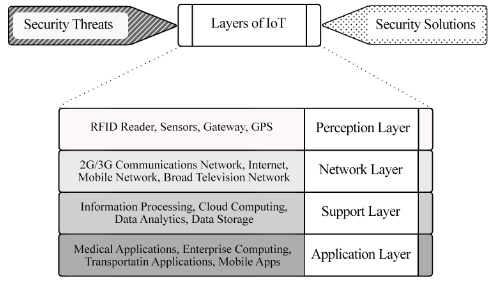
\includegraphics[scale=0.65]{layers_IoT.png}
%\caption{Architecture d'un système IoT proposée par Leloglu \cite{Leloglu2017}}
%\label{prov}
%\end{figure}

\begin{table}[!ht]
    \center
    \begin{tabular}[b]{|c|p{12cm}|}
    \hline
		Niveau dans le système &  Exemples de technologies, systèmes et équipements y opérant\\
	\hline
Couche perception & Caméras, microphones, capteurs, GPS et divers systèmes embarqués mesurant et interagissant avec l'environnement qui leur est extérieur (montres intelligentes, détecteurs, etc.), ainsi que la technologie RFID. Côté software : OS adapté aux systèmes embarqués tels que Contiki, tinyOS, LiteOS, etc.\\
	\hline
Couche réseau & Réseaux de capteurs, réseau mobile 2G/3G, réseaux classiques tel que Internet (IP).\\
	\hline
Couche support & Cloud, centre de traitement des données, base de données et autres technologies et supports permettant d’agréger, stocker et analyser les données (\textit{Big Data})\\
	\hline
Couche application & Applications relatives aux smarthomes (interfaçage avec l'utilisateur, optimisation de son quotidien, etc.), applications médicales (surveillance de patients, aides aux invalides, etc.), sociales et structurelles (smartcity : parkings intelligents, etc.), scientifiques (études des mesures, détection de catastrophes, etc.) et industrielles (arrosage de plants, transport, etc.)\\   
  \hline
    \end{tabular}
    \caption{Architecture d'un système IoT proposée par Leloglu \cite{Leloglu2017}}
    \label{IoT_model_desc}
\end{table}

\newpage

    \begin{figure}[!h]
       \noindent\makebox[\textwidth]{%
       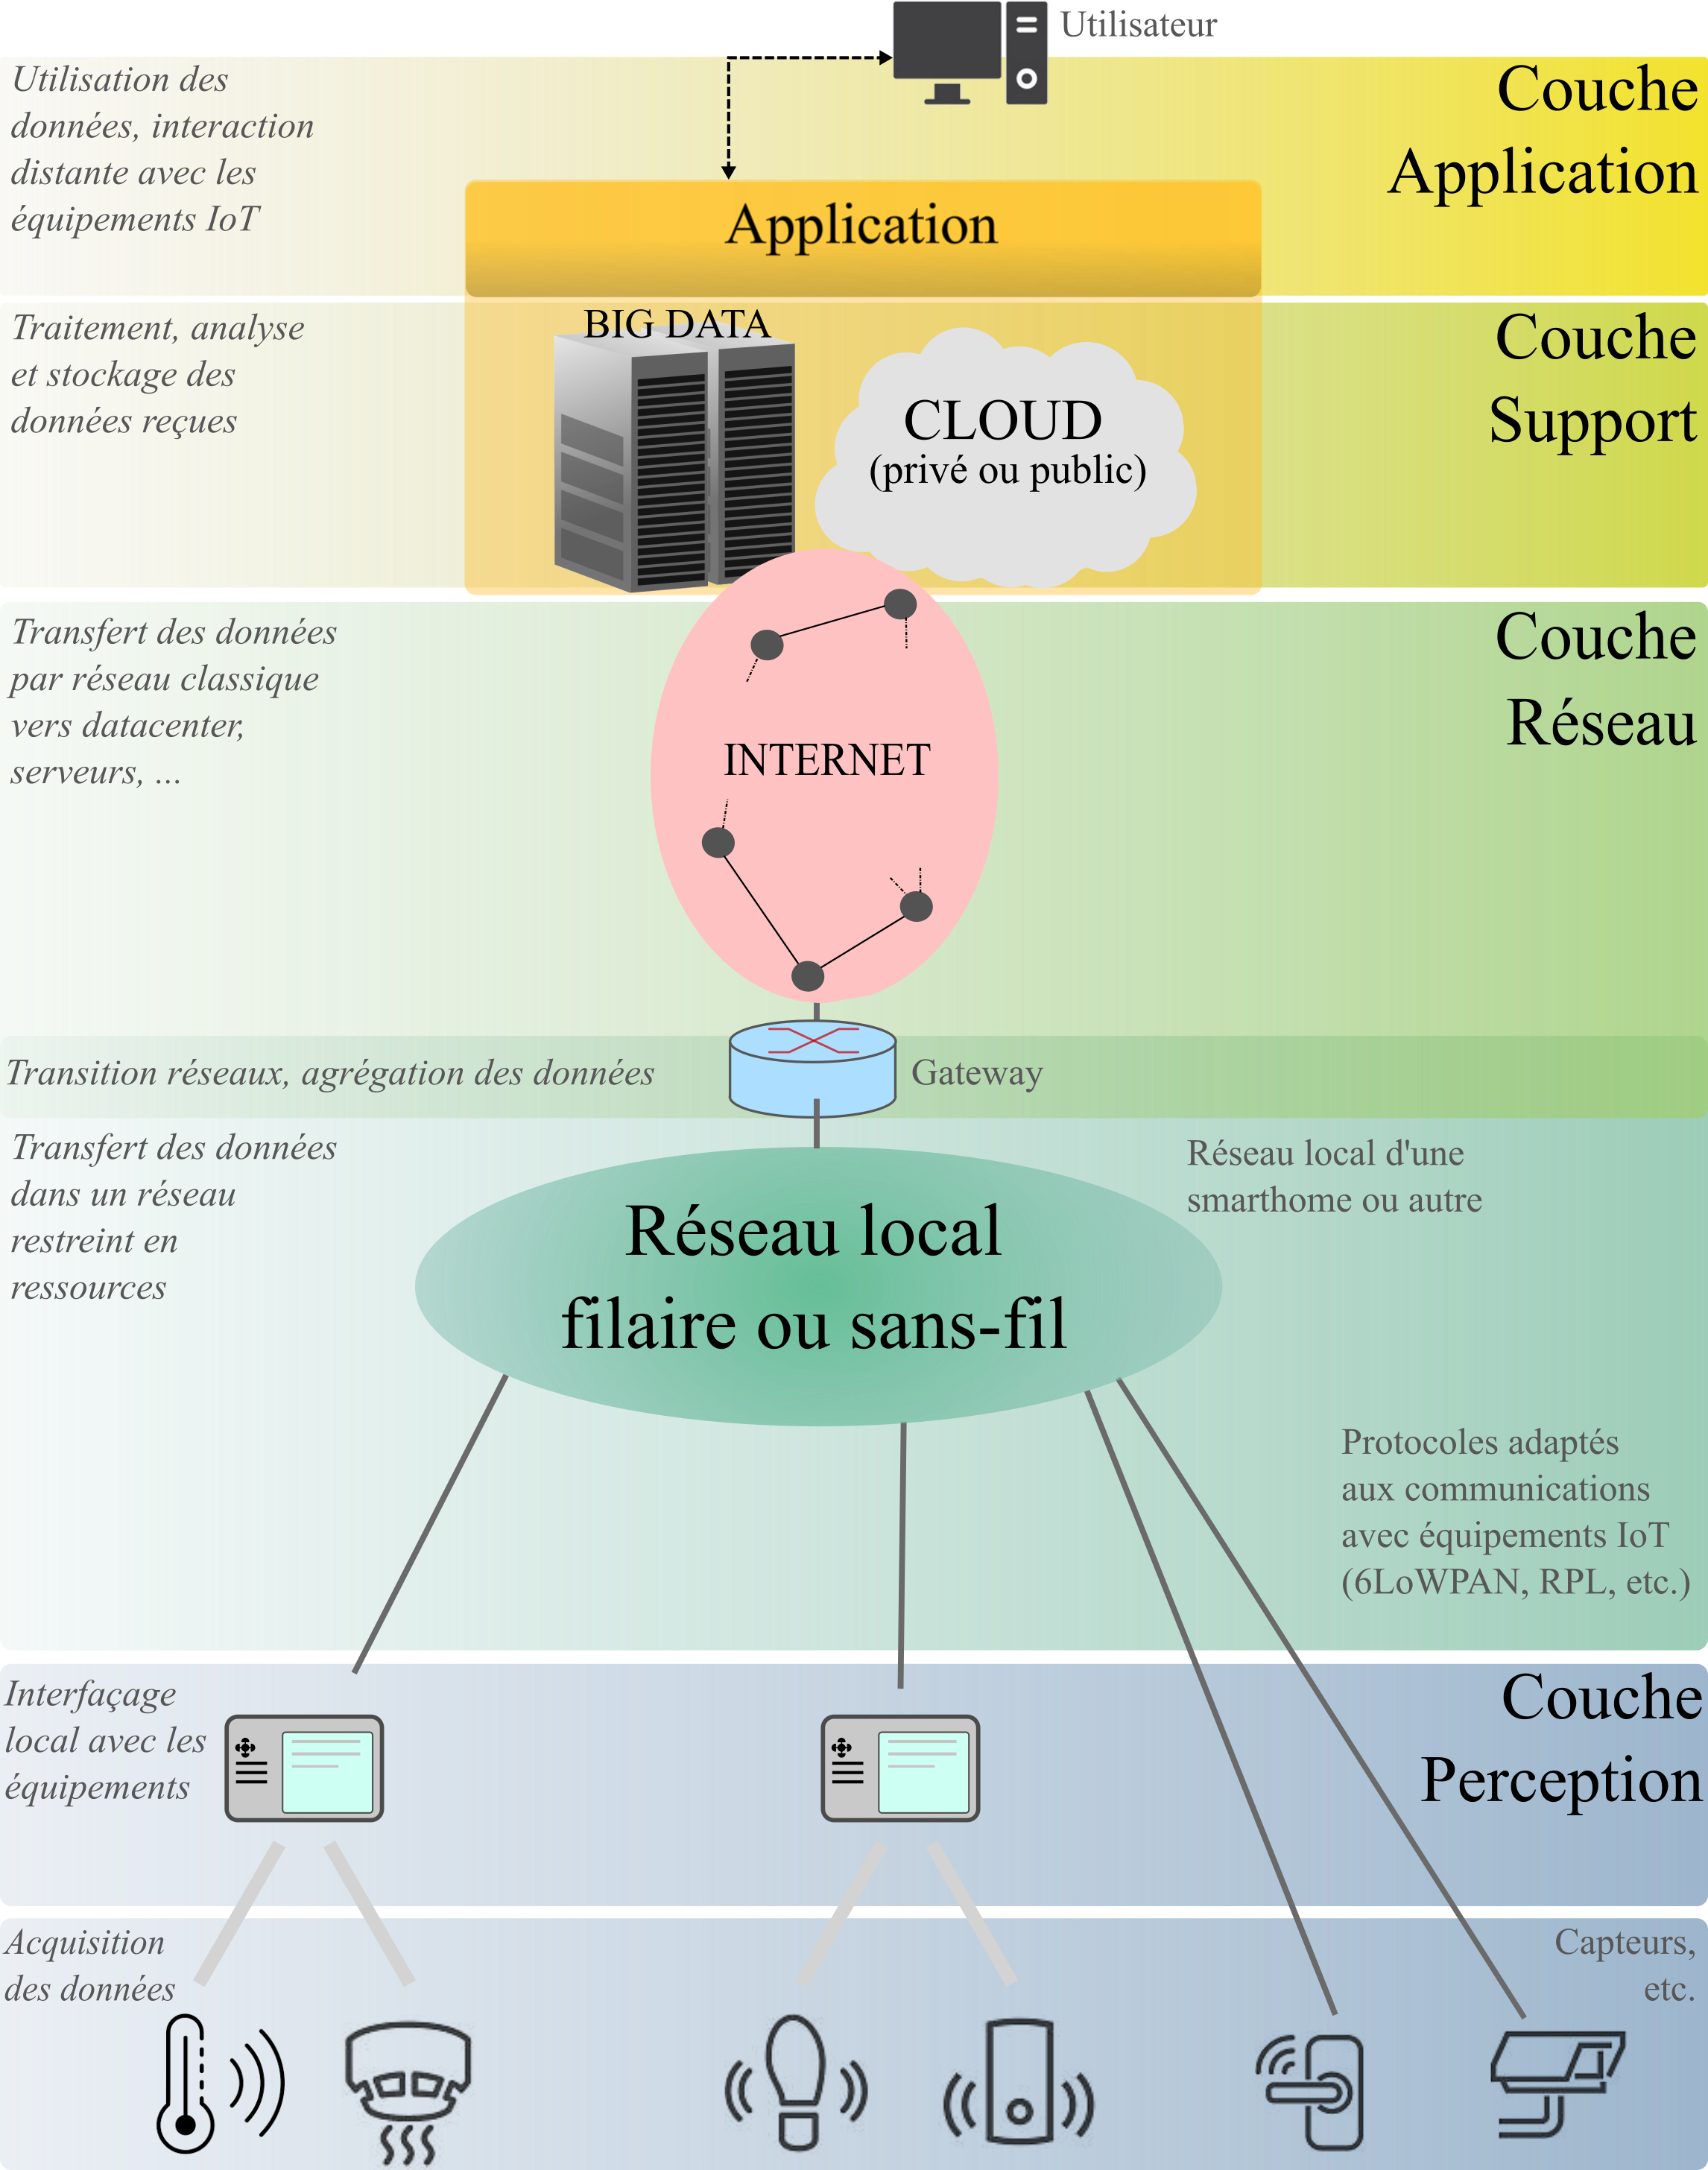
\includegraphics[width=0.67\textwidth]{IoT_sec_layers.png}}
       \caption{Schématisation des couches considérées pour un système utilisant des équipements IoT}
       \label{IoT_model_scheme}
    \end{figure}
    
\newpage
%\subsection{Les attaques courantes}
\subsection{Les archétypes d'attaques courantes}

Plusieurs schémas d'attaques peuvent être distingués, exploitant ou non des vulnérabilités recensées dans la \wordlink{vuln_IoT}{section}. Ces scénarios d'attaques typiques sont classés en fonction de la couche dans laquelle ils opèrent, selon Makhdoom et al. \cite{Makhdoom2018} et Leloglu \cite{Leloglu2017}.


\subsubsection{Sur la couche perception}

\par Drainage de batterie (\textit{Depletion-of-Battery attack}) : en apparence justifiée car il s'agit d'un scénario légitime du point de vue de l'utilisation, ce type d'attaque porte préjudice à un nœud en le bombardant de requêtes qu'il doit traiter car considérées comme légitimes. Cela empêche le nœud de passer en mode veille pour préserver de l'énergie, et peut mener à l'extinction de celui-ci une fois sa source d'énergie épuisée.\\

\par Sabotage du nœud (\textit{Node capturing/cloning}) : un attaquant peut attenter physiquement au système : il est possible qu'il accède à un nœud parmi ceux dispersés dans un réseau de capteur par exemple. Il lui est donc potentiellement possible de le corrompre ou le remplacer physiquement par un nœud intrus qui effectuera un travail dissimulé.\\

\par Brouillage radio (\textit{Signal/Radio jamming}) : un type d'attaque DoS qui vise à occuper le canal (sans-fil) au moment où des nœuds souhaitent également émettre, brouillant les communications.\\

\par Écoute clandestine (\textit{Eavesdropping}) : dans le cadre des communications sans-fil, un attaquant peut placer physiquement ou corrompre un nœud alors clandestin qui lui permet d'écouter les informations passant par ce canal. Ces informations peuvent être sensibles, telles que des mots de passe transmis en clair par d'autres équipements. Outre cela, le simple fait de savoir quand des informations sont émises sur le canal peut profiter à un attaquant, par exemple en l'aidant à évaluer quand une maison est occupée ou non.\\

\par Attaque par intrusion (\textit{(Semi-)Invasise intrusions})\footnote{\url{https://www.cl.cam.ac.uk/~sps32/semi-inv_def.html}} : par l'étude des variations de certains indicateurs tels que le voltage, le signal de l'horloge, etc., un attaquant peut inférer les opérations qu'un microcontrolleur effectue. Il est aussi possible de déduire certaines valeurs stockées dans la mémoire sensée rester privée telles que les clés maitres de chiffrement (AES ou autre). En appliquant des fluctuations physiques, il est aussi possible de faire en sorte que le CPU exécute au final une autre opération que celle attendue.\\
%https://www.cl.cam.ac.uk/~sps32/semi-inv_def.html

\par Mises à jour faussées : des implémentations mal faites des mécanismes d'authentification peuvent aider un attaquant à soit maintenir une version du firmware obsolète, soit faire passer une mise à jour falsifiée comme provenant du constructeur officiel de l'équipement. Les patchs relatifs à la sécurité peuvent ainsi être bloqués, et les failles qu'ils corrigeaient laissées exploitables.



\subsubsection{Sur la couche réseau}

\par \textit{Spoofing} : effectuée par le biais de paquets forgés, ce type d'attaque vise à usurper une identité renseignée comme source du paquet falsifié. Une attaque de ce type est rendue possible à plusieurs niveaux\footnote{\url{https://en.wikipedia.org/wiki/Spoofing_attack}} des communications, dès qu'aucun mécanisme n'est mis en place pour authentifier les entités communiquant (on parle d'\textit{ARP, IP, MAC, ... spoofing}). L'usurpation d'identité permet des attaques plus concrètes telles que les \textit{MITM attacks} décrites ci-dessous.\\

\par \textit{Selective Forwarding} : un nœud infecté ou malicieux introduit dans le réseau peut influencer celui-ci quand il est question de retransmettre des paquets (il effectue un travail de routage). Selon une certaine procédure créée pour manipuler artificiellement le trafic dans un sens profitant à l'attaquant, le nœud ne retransmet que les paquets qu'il sélectionne. Afin que ce ne soit pas trop évident de déceler le subterfuge, il n'arrête pas toutes les retransmissions.\\

\par Attaque de Sybil : un nœud malicieux gère plusieurs identités simultanément, propres ou en se faisant passer pour un autre nœud. Du point de vue des nœuds légitimes, ce sont donc plusieurs équipements distincts (simultanément ou représenté tour par tour). Une panne ou une attaque impactant la disponibilité d'autres nœuds peut ainsi être masquée par ce procédé.\\

\newpage

\par \textit{Sinkhole/Blackhole attack} : l'attaque consiste à consommer les ressources de nœuds voisins dans le rayon d'émission d'un nœud infecté. Cela se fait essentiellement en occupant le canal radio, brouillant les transmissions légitimes. Il en résulte une consommation d'énergie anormalement élevée pour les nœuds dans cette zone, attribuée aux retransmissions alors nécessaires.\\

\par \textit{Wormhole} : cette attaque cible les protocoles de routages, introduisant une confusion dans le calcul des routes. Un nœud infecté va transmettre un paquet qu'il est censé router, directement vers un autre nœud éloigné en établissant un tunnel invisible pour le protocole de routage. Ainsi, des nouvelles routes vont apparaître, donnant l'illusion que les deux nœuds sont proches, ce qui pour un protocole de routage se basant sur la distance entre deux nœuds constituera une nouvelle meilleure route (qui ne l'est en réalité pas du tout).\\

\par \textit{Man-in-the-Middle attack (MITM)} : forme d'eavesdropping où l'attaquant s'interpose entre deux nœuds voulant communiquer légitimement. Il opère de façon à ce que la communication ait lieu normalement du point de vue des deux autres intervenants, mais de sorte que chacun communique avec lui qui joue le rôle d'intermédiaire. Il peut alors accéder au contenu de tous les échanges et le manipuler pour en tirer des informations confidentielles et influencer le déroulement de la communication.\\

\par \textit{Hello-flood attack} : inondation du canal par des messages inutiles d'annonces de voisin qui demandent une réponse de la part des nœuds qui le reçoivent (générant ainsi davantage de trafic).\\

\subsubsection{Sur la couche support et application}

\par Altération/exploitation des données : comme ces couches manipulent des données issues de ce que les équipements ont mesuré et capté, elles peuvent être sensibles et doivent être protégées. Un attaquant qui met la main sur ces données pourrait d'une part les corrompre et d'autre part les analyser et les exploiter afin de mener une autre attaque contre les utilisateurs. Par exemple, il pourrait dégager à partir des données enregistrées quelles sont les plages horaires pendant lesquelles un domicile n'est pas occupé et donc trouver une fenêtre de liberté pour une approche physique. De plus,  ces données ne sont plus directement sous le contrôle de l'utilisateur (stockées dans les machines d'une entreprise), cela peut donc être problématique et mener à une atteinte à sa vie privée (revente  illégale d'informations à une compagnie tierce, etc.).\\

\par Attaques de déni de service (\textit{DoS}, \textit{DDoS}) : les compagnies qui hébergent les services repris dans les couches support et application (traitement des données, accès aux serveurs, etc.) sont elles aussi susceptibles de se faire attaquer directement. Les attaques DoS (ou DDoS comme illustré avec Mirai en introduction de cette section) sont courantes et peuvent complètement interrompre la disponibilité de ces services par différent biais (congestion, mise à l'arrêt des machines).\\

\par Injection de code : l'attaquant utilise des failles dans les applications pour injecter et faire exécuter son propre code écrit à des fins malicieuses. Cela se fait notamment sur les bases de données (injection SQL). Une injection peut résulter en l'installation d'un malware, des requêtes illégitimes effectuées sur les bases de données, un gain de privilèges dans le système pour l'attaquant ou encore rendre possible du \textit{cross-site scripting}\footnote{\url{https://en.wikipedia.org/wiki/Cross-site_scripting}}.\\

\par \textit{Sniffers/loggers} : les attaquants récoltent un maximum des données utilisées et transitant (par exemple lors des échanges avec l'utilisateur par le biais de l'application) afin d'en tirer des informations de valeur (bien que cela soit rendu plus difficile par le chiffrement). Il peut s'agir d'identifiants, de mots de passes, d'emails, etc.\\

\par \textit{Session Hijacking} : les attaquants exploitent des failles dans les processus d'authentification et gestion de session afin d'interférer dans les échanges et obtenir des accès privilégiés à des ressources. Cela se fait principalement via les cookies.\\

\par Ingénierie sociale : l'attaquant extrait des informations ou interagit directement avec l'utilisateur inaverti pour obtenir des identifiants ou autre en fonction de l'application à laquelle l'utilisateur accorde sa confiance.

\newpage


\subsection{Ressources, solutions et outils existants}
\label{scanners}

\subsubsection{Le travail d'OWASP}

La fondation \href{https://www.owasp.org/index.php/Main_Page}{OWASP} (\textit{The Open Web Application Security Project}) est une organisation à l'échelle mondiale qui aspire à améliorer la sécurité informatique des systèmes et logiciels. L'IoT étant en plein essor, \href{https://www.owasp.org/index.php/OWASP_Internet_of_Things_Project}{un projet} a vu le jour sur la plateforme web, décrit comme \og conçu pour aider les fabricants, développeurs et utilisateurs à mieux comprendre les problèmes sécuritaires liés à l'IoT, et pour permettre aux utilisateurs de prendre de meilleures décisions relatives à la sécurité quand ils déploient et travaillent avec des technologies de l'IoT \fg .
Ainsi, plusieurs sous-projets plus spécifiques sont destinés à peupler le projet principal, certains étant encore actuellement en développement.\\

L'équipe travaillant sur le projet a établi \href{https://www.owasp.org/index.php/Principles_of_IoT_Security}{une liste} des principes relatif à la sécurité dans l'IoT. Plusieurs guides ont également été écrits, orientés chacun selon un point de vue différent : pour le fabricant, le développeur et l'utilisateur. D'autres ressources écrites sont disponibles, mais encore aucun outil développé autour de la sécurité n'a vu le jour comme c'est le cas pour d'autres domaines (les applications web particulièrement puisque originellement l'organisation ciblait ce secteur).	 

\subsubsection{La standardisation de protocoles adaptés sécurisés}

\par La \wordlink{IoT_prot}{sous-section} présentait les protocoles utilisables dans l'IoT, adaptés aux restrictions des équipements qui ne permettent pas toujours une compatibilité avec la \textit{pile TCP/IP} classique. Lors de la conception de ces protocoles, la composante sécurité a été prise en compte et des mécanismes y ont été introduits pour l'assurer (ou alors des chercheurs ont fait ce travail par la suite).\\

\par 6LowPAN propose déjà des mécanismes utiles pour garantir la sécurité \cite{wiki6lowpan}. Pour éviter les attaques par fragmentation, les options d'en-têtes \textit{Timestamp} et \textit{Nonce} sont un premier rempart. Des chercheurs ont également élaboré une version allégée de la suite de protocoles IPsec afin de garantir des communications sécurisées d'un nœud à l'autre dans un réseau 6LowPAN \cite{Huichen2016}. D'autres chercheurs présentés dans le même article ont proposé un système d'établissement de connexion sécurisée à partir d'un échange de clés.\\

\par RPL, utilisé pour le routage dans les réseaux de capteurs notamment au dessus de 6LowPAN, dispose également de mécanismes de protection. Il s'agit dans ce cas de garantir que quand un nœud sélectionne son parent pour rejoindre la topologie, ce dernier soit un nœud légitime (éviter le \textit{spoofing}). Des solutions d'autres chercheurs sont présentées par Huichen \cite{Huichen2016} afin de sécuriser la génération des tables de routage dans RPL. Un exemple est un schéma de topologie authentifiée appelée TRAIL (\textit{Trust Anchor Interconnection Loop}) qui permet la découverte et l'isolation des nœuds falsifiés et où chaque nœud peut, en envoyant un message particulier, valider son chemin jusqu'à la racine.\\

\par CoAP, tout comme son homologue HTTP, peut s'appuyer sur une couche intermédiaire plus basse pour assurer un transport sécurisé (chiffré pour préserver la confidentialité). Il s'agit de DTLS (\textit{Datagram Transport Layer Security}), un équivalent de TLS plus adapté aux communications d'équipements restreint. La principale différence réside dans le fait que TLS soit basé sur TCP, au contraire de DTLS qui l'est sur UDP, toujours dans l'optique d'utiliser le minimum de ressources. CoAP offre le choix entre quatre modes relatifs à la sécurité : \textit{NoSec}, \textit{PreSharedKey}, \textit{RawPublicKey} et \textit{Certificate}.

\subsubsection{La détection des équipements en réseau et de leurs vulnérabilités}

Face à un réseau réel, disons local à une habitation possédant des équipements connectés (c-à-d orientée smarthome), il est difficile de se faire une idée de tous les objets y étant connectés et de quelles sont leurs fonctionnalités. Des outils sont nécessaires afin de découvrir le réseau et établir quels équipements peuvent potentiellement être la cible d'attaques. Il en existe une flopée (\href{https://sectools.org/}{sectools.org} en maintient un classement fourni), libres ou commerciaux, possédant une interface graphique ou non, fonctionnels sur des OS variés. Outre ces logiciels complets aux champs d'action assez étendu, des outils de scanning plus spécifiques à des cibles (routeurs, serveurs, ...) et services (Web, SQL, mail, ...) sont trouvables dans des dépôts dédiés sous la forme de scripts (\href{https://github.com/We5ter/Scanners-Box}{Scanners-box} \footnote{\url{https://github.com/We5ter/Scanners-Box}} est dédié à leur référencement). Des exemples sont donnés ci-dessous, classés en deux catégories \cite{Leos2014} en fonction de la manière dont le scan est effectué. Une attention particulière est portée aux outils dédiés à la détection des failles sur les équipements IoT d'un réseau s'il en existe qui y soient dédiés.

\paragraph{Le scan passif et la prise d'empreintes}

L'objectif est d'en apprendre un maximum sur les équipements connectés au réseau sans les interpeller directement. Cela se fait en écoutant toutes les transmissions passant sur un média utilisé par ces équipements, les capturant, les stockant et les agrégeant. Cela est donc assimilable à la pratique du sniffing. L'utilisation qui est faite de ces données varie en fonction de l'application : soit elles sont étudiées telles quelles car c'est le trafic qui est intéressant (\href{https://en.wikipedia.org/wiki/Packet_analyzer}{analyseurs de trafic}), soit elles sont utilisées pour faire de la \og prise d'empreinte\fg \ (\href{https://en.wikipedia.org/wiki/TCP/IP_stack_fingerprinting}{\textit{TCP/IP stack, OS fingerprinting}}) afin de caractériser les nœuds du réseau, soit les deux. Il peut également y avoir, suite à la phase d'écoute passive, des actions entreprises (par exemple si le processus a déterminé qu'un hôte présente une faiblesse exploitable).\\

\par Un analyseur de paquet populaire est Wireshark, qui utilise l'API \textit{pcap} pour capturer les paquets transitant par le réseau sur lequel une interface désignée est placée en mode promiscuité (c-à-d fait remonter au système tous les paquets qui lui parviennent). Beaucoup d'autres utilitaires de capture (Kismet, tcpdump, ngrep, etc.) utilisent l'API \textit{pcap}, implémentée dans la librairie \textit{libcap} (systèmes UNIX) ou WinPcap (port de libcap vers Windows), il s'agit donc d'une ressource importante. Wireshark permet un filtrage assez fin des lots de paquets capturés (plus d'un millier de protocoles reconnus), permettant une grande flexibilité en fonction du but de la capture (debug, recherche d'une information, surveillance du trafic, etc.).\\

\par Les logiciels destinés à la capture d'empreintes et uniquement à cela sont assez peu nombreux (la plupart intègrent d'autres fonctionnalités actives). \href{http://lcamtuf.coredump.cx/p0f3}{p0f}\footnote{\url{http://lcamtuf.coredump.cx/p0f3}} est l'outil minimaliste le plus efficace. Il utilise diverses métriques extraites des en-têtes IPv4/6, des en-têtes TCP, des dynamiques observables dans le 3-way handshake de TCP et des données exploitables au niveau de la couche application (HTTP, SMTP, FTP, etc.). Combinées à une base de données de signatures récupérées expérimentalement, ces mesures permettent de déduire quels systèmes opèrent derrière les nœuds du réseau communiquant (là où un outil comme Nmap peut en être incapable). Outre cela, p0f est capable de déduire d'autres informations :

\begin{itemize}
\vspace{0.2cm}
\item[$\bullet$] présence d'un pare-feu, d'un système de NAT ou \textit{load balancer}, de proxy applicatifs
\vspace{0.2cm}
\item[$\bullet$] mesures du temps d'activité d'un système, sa distance (grâce au TTL), ses préférences au niveau de la langue, etc.
\vspace{0.2cm}
\item[$\bullet$] les services utilisés par les clients et serveurs qui déclarent des champs comme X-Mailer ou User-Agent
\end{itemize}
~
\par D'autres outils existent, leurs fonctionnalités s'étendant au-delà de ce qui est considérable comme outil passif. On peut citer notamment :
\begin{itemize}
\vspace{0.2cm}
\item[$\bullet$] \href{http://www.ettercap-project.org/}{Ettercap}\footnote{\url{http://www.ettercap-project.org/}} utilise la capture de paquets pour intercepter des informations sensibles, et d'autres opérations avec pour but final d'effectuer une attaque de type \textit{Man-In-The-Middle} (MITM)
\vspace{0.2cm}
\item[$\bullet$] \href{https://scapy.net/}{Scapy}\footnote{\url{https://scapy.net/}} et \href{https://github.com/phaethon/kamene}{Kamene} (fork du projet), des utilitaires en Python, permettent la capture et le reforgeage de paquets, la prise d'empreintes, le lancement d'attaques, etc. (le tout de façon modulable)
\end{itemize}
~\\

\newpage

\paragraph{Le scan actif}

\par Ces logiciels tentent d'établir des connexions avec les hôtes à analyser, à la recherche d'un service répondant donc potentiellement ouvert, non protégé et dont il est possible de soutirer des informations. Une liste de numéros de ports pertinents est construite par le scanneur, utilisée par ce dernier lors de l'analyse des hôtes qu'il trouve dans le réseau. Cette technique basique est appelée \href{https://fr.wikipedia.org/wiki/Balayage_de_ports}{balayage de port}.   Se servant de ces scanneurs comme appoint, les \href{https://fr.wikipedia.org/wiki/Scanneur_de_vuln\%C3\%A9rabilit\%C3\%A9}{scanneurs de vulnérabilités} vont plus loin en tentant de découvrir pour chaque hôte analysé les failles de sécurités auxquelles ils sont exposés (au niveau d'une application, du système d'exploitation ou des interfaces réseaux).\\

\par L'outil \href{https://nmap.org/}{Nmap}\footnote{\url{https://nmap.org/}} est dédié au balayage de ports et à l'acquisition directe d'informations (version, composants matériels utilisés, etc.) concernant le système et les services ouverts d'un hôte analysé. La détection de vulnérabilités est rendue possible grâce aux interactions scriptées avec la cible en utilisant le Nmap Scripting Engine (NSE), un exemple de module Nmap y étant dédié est \href{https://www.computec.ch/projekte/vulscan/}{Vulscan.nse}. Nmap a d'autres fonctionnalités pratiques telles qu'une interface graphique complète (\href{https://nmap.org/zenmap/}{Zenmap}) et la personnalisation des formats de sorties pour les résultats (filtrage, langages balisés, etc.).\\

\par \href{http://www.openvas.org/}{OpenVAS}\footnote{\url{http://www.openvas.org/}} est une branche du projet \href{https://www.tenable.com/products/nessus/nessus-professional}{Nessus}, ce dernier étant passé sous licence commerciale. Ce sont les frameworks pour la détection de vulnérabilités sur un réseau les plus populaires. Tenable$^{®}$ (qui possède Nessus) propose des \href{https://www.tenable.com/solutions/iot}{services de scan dédiés aux équipements IoT} utilisés dans l'industrie, mais OpenVAS n'offre rien de similaire.\\

\par Le cas de \href{https://cisofy.com/lynis/}{Lynis}\footnote{\url{https://cisofy.com/lynis/}} est un peu particulier. Effectivement, en opposition aux scanneurs en réseau comme OpenVAS, il s'agit d'un scanneur de vulnérabilités à lancer sur l'hôte à analyser. Cela permet une inspection beaucoup plus en profondeur des services et des vulnérabilités qu'il présente. Il tourne sur presque tous les systèmes UNIX et même sur un système limité tel qu'une carte Raspberry Pi ou un équipement relatif à l'IoT qui est capable de supporter le même type de charge. Lynis peut donc être un outil intéressant si on possède le contrôle de l'équipement à analyser (légitimement ou non).\\

\par Dédié à la détection des vulnérabilités des équipements IoT, \href{https://github.com/rapid7/IoTSeeker}{IoTSeeker}\footnote{\url{https://github.com/rapid7/IoTSeeker}} est un outil libre et écrit en Perl, supporté par les systèmes Linux/Mac OS. Il est axé sur les vulnérabilités d'authentification, la découverte de mots de passe laissés par défaut par les utilisateurs imprudents (sur base des listes des identifiants par constructeur évoquées dans la \wordlink{motiv_IoT}{sous-section}).\\

\par \href{https://github.com/threat9/routersploit}{Routersploit}\footnote{\url{https://github.com/threat9/routersploit}} est un framework dédié à la détection et l'exploitation de failles dans les systèmes embarqués. Comme son nom l'indique, la cible est davantage les routeurs que les équipements de l'IoT, cependant quelques modules ciblent notamment les caméras et d'autres équipements connectés insolites (projecteur, laveur de laboratoire). L'outil de pénétration \href{https://github.com/zdresearch/OWASP-Nettacker}{Nettacker} développé par OWASP, dont le but est le soutirage et l'agrégation d'informations d'une cible pour en dresser une liste des failles de sécurité, promet également la sortie future d'un module spécifique à l'IoT.

%------------- PARE FEUX + IoT -------------


%------------- IMPLEM -------------

%------------- CCL -------------

\newpage

\section{Développement d'une application \textit{IoTMonitor} - introduction et concepts}
%---------------- Intro
\subsection{Présentation générale}

\subsubsection{Contexte et environnement ciblé}

Ce travail englobe la thématique de la sécurité des équipements en réseau dans l'environnement domestique, en mettant l'accent sur les différents types de pare-feux. Effectivement, ces derniers peuvent palier en partie aux faiblesses récurrentes des équipements IoT qui peuplent les réseaux domestiques. L'aboutissement final du projet est de développer un outil qui puisse contribuer à la protection de ces réseaux. Cependant, l'analyse de trafic avancée (au delà du simple pare-feu à état) telle qu'utilisée dans les solutions commerciales est une technologie non triviale qui sort des limites de ce projet (théorie de \textit{machine learning}, construction de base de données de signatures, etc.). À l'inverse, se limiter à un simple pare-feu à état ciblant un protocole de l'IoT peut sembler réducteur vis-à-vis de toutes les menaces planant sur ces équipements qu'un tel pare-feu ne pourrait contrer.\\

\par La \wordlink{scanners}{sous-section} met en évidence quelques outils qui peuvent aider à analyser le réseau domestique et détecter les failles exploitables des équipements qui le peuplent. Ces \textit{scanners}, conjugués à des systèmes de prévention d'intrusion \textit{NIDS}, permettraient d'améliorer grandement la sécurité du réseau domestique, tout en n'effectuant aucune tâche de filtrage direct du trafic comme le ferait un pare-feu en bordure du réseau. En découle l'idée motrice de l'application à développer : prodiguer un outil permettant l'\textbf{analyse}, la \textbf{surveillance} et l'\textbf{agrégation des caractéristiques des équipements (adresses IP/MAC, ports ouverts, etc.)} d'un réseau domestique, basé sur des \textbf{scanneurs} existants ciblant \textbf{différents aspects} de sa sécurité. Le système doit donc être conçu de façon modulaire, de sorte que l'\textbf{intégration d'un nouveau scanneur} ne requiert comme travail que la traduction (parsing) de la sortie dudit programme vers des actions et éléments interprétables par l'application.     \\

\par Par exemple, l'application pourrait intégrer des scanneurs tels que présentés dans la \wordlink{scanners}{sous-section}. Parmi ceux-ci \textit{nmap}, \textit{IoTSeeker}, etc. qui interrogent directement les équipements (dits actifs) et des programmes de prise d'empreintes/analyse de trafic tels que \textit{Snort}, \textit{p0f}, etc. (dits passifs). Chacun de ces programmes fournit un feedback sur sa sortie, que ce soit une fois son exécution terminée ou de façon continue jusqu'à interruption manuelle de l'exécution. Une fois parsées, les informations obtenues peuvent servir à alimenter une représentation virtuelle du réseau maintenue par l'application (renseignant les caractéristiques des équipements qui le peuplent) ou constituer une alerte à faire remonter jusqu'à l'utilisateur si une faille ou menace est détectée.\\

\par Par programme il est entendu : \textit{un programme ou script installé et fonctionnel sur le système, exécutable depuis un terminal et dont la sortie est récupérable}. Le framework d'intégration définit comment ajouter ces programmes à l'environnement de l'application, prodiguant une surcouche telle qu'il n'est nécessaire de définir que les éléments suivants :\\
\begin{itemize}
\item[$\bullet$] la \textbf{commande} liée au programme telle qu'utilisée pour y faire appel depuis un terminal
\vspace{0.2cm}
\item[$\bullet$] quels \textbf{paramètres du programme} utilisés parmi ceux passables en ligne de commande et la façon d'y associer des valeurs (\textit{schéma} de paramètres)
\vspace{0.2cm}
\item[$\bullet$] la \textbf{méthode de traitement} de la sortie du programme (parsing) pour en inclure les résultats dans l'application
\end{itemize}


\vspace{0.2cm}

\subsubsection{Objectifs de l'outil}

\paragraph{La surveillance automatique du réseau domestique}

Une manipulation aisée des programmes à utiliser pour surveiller le réseau est essentielle. L'utilisateur doit pouvoir sélectionner et configurer les programmes qu'il souhaite pour défendre son réseau parmi ceux disponibles. Une fois cette sélection opérée, les programmes choisis devraient être maintenus dans une structure où leur exécution, la récupération de leur sortie et le parsing de ces dernières sont entièrement automatisés. L'utilisateur n'ayant alors qu'à agir sur cette structure pour contrôler l'état de la surveillance de son réseau. La gestion du travail des programmes qui y sont maintenus est entièrement automatisée et ne requiert pas d'interaction avec l'utilisateur. L'application peut alors agir de façon autonome et effectuer sa tâche de surveillance en fond continuellement. Ladite structure est un objet appelé \textbf{Routine} dans l'application.

\newpage

\paragraph{La représentation du réseau}

Puisque n'importe quel programme peut potentiellement être intégré dans l'environnement de l'application, les sorties sont totalement arbitraires. Cependant, il est très probable que celles-ci contiennent des informations relatives aux hôtes sur le réseau analysé : adresses MAC, IP, nom d'hôte, etc. Un objectif de l'application est de regrouper toutes ces informations afin de construire une carte virtuelle du réseau la plus fidèle possible. Cette carte est appelée \textbf{Netmap} et doit être consultable par l'utilisateur de façon à ce qu'il ait une vision synthétique mais complète de l'état de son réseau. L'utilisateur doit également pouvoir interagir avec cette carte en créant et modifiant des informations associées aux hôtes, afin d'assister ou corriger la récolte automatique d'informations.

\paragraph{La détection de menaces}

Certains programmes intégrés à l'application sont conçus pour trouver des failles existantes aux hôtes du réseau. Une fois les sorties de ces programmes parsées, les menaces détectées doivent être remontées jusqu'à l'utilisateur et archivées dans l'application. Les notifications à l'utilisateur, s'il n'est pas directement en train d'utiliser l'application, se font par un email récapitulatif de la menace trouvée. Pour en consulter les détails par la suite, les menaces associées à un hôte doivent être consultables dans l'application même.

\paragraph{La conception d'un framework d'intégration}

Puisque l'application fonctionne en se basant sur des programmes extérieurs arbitraires, il est nécessaire de définir un cadre assez rigoureux pour les intégrer au système de sorte à pouvoir manipuler leur exécution et leur passer des paramètres. Cela se fait via une surcouche d'abstraction désignée par le terme \textbf{Module}. Dans les faits, il s'agit d'une classe à écrire en Python héritant d'une classe abstraite (faisant office de framework). Deux types de Modules sont envisagés pour abstraire un programme en fonction de son schéma d'exécution, décidant de la classe abstraite à sous-classer. Ces deux archétypes sont détaillés dans la \wordlink{abstrmodel}{sous-section}.

\paragraph{L'utilisation en environnement restreint}

L'application doit pouvoir être utilisée telle quelle depuis un équipement connecté au réseau domestique, similaire ou supérieur en terme de ressources à une carte Raspberry PI. Également, l'application devrait pouvoir être pleinement utilisée dans un environnement non graphique, par exemple sur la carte Raspberry depuis une connexion SSH distante. Effectivement, comme le travail de surveillance effectué par l'application nécessite une machine continuellement active, il est préférable pour l'utilisateur qu'elle soit peu consommatrice. Une carte Raspberry PI 3 dédiée à l'utilisation de l'application devrait être suffisante.

\newpage
%---------------- Concepts

\subsection{Composants du système de surveillance}
\label{compapp}

Afin de mieux visualiser les différents éléments qui composent le cœur de l'application, une maquette d'interface graphique a été élaborée. Celle-ci représente ce à quoi devrait correspondre l'écran de gestion principal de l'application. Effectivement, afin de pouvoir être utilisée dans un contexte restreint (tel que sur une carte Raspberry PI), l'application a d'abord été dotée d'une interface en ligne de commande en priorité (voir \wordlink{justifinter}{point}). Une partie des composants principaux sont repris dans la 
\wordlink{gui}{figure}.

\begin{figure}[!ht]
   \begin{adjustwidth}{-\oddsidemargin-1in + 0.5cm}{-\rightmargin}
     \centering
     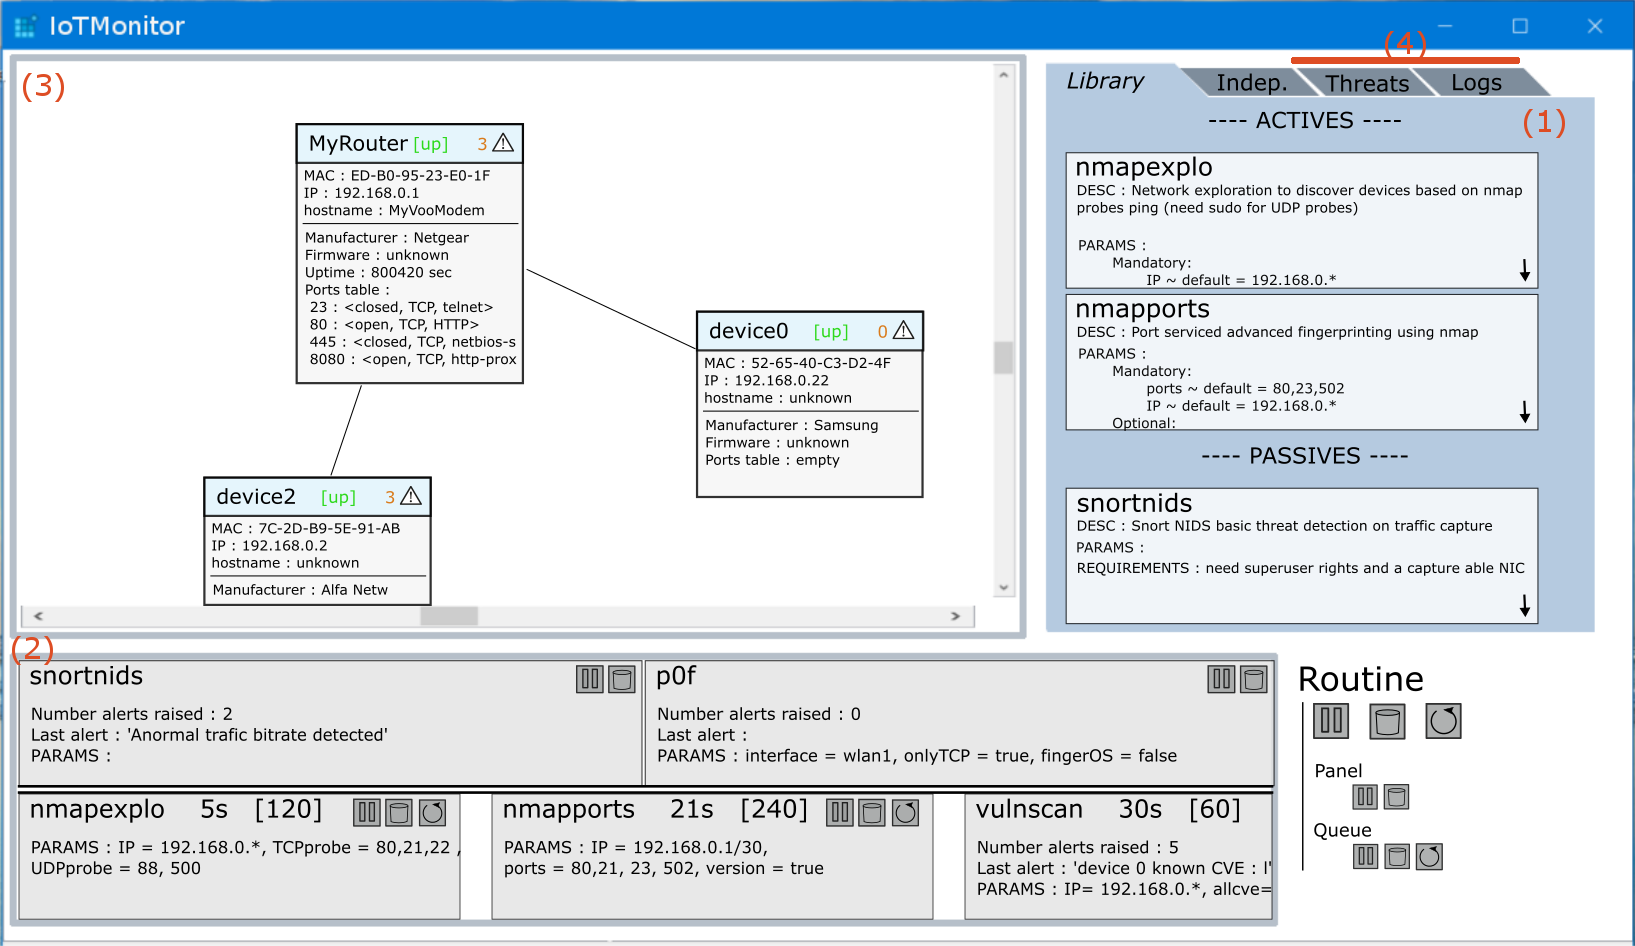
\includegraphics[width=\paperwidth - 1cm]{maqGUI}
     \caption{Maquette GUI de l'application en reprenant les principaux éléments}
     \label{gui}
   \end{adjustwidth}
   \
\end{figure}

\subsubsection{Modules actifs et passifs - abstraction des programmes}

Les Modules constituent la couche d'abstraction pour les programmes sous-jacents et sont régis par un framework spécifique à l'archétype attribuable au programme. On distingue deux archétypes de programmes selon leur schéma d'exécution propre :\\
\begin{itemize}
\item[$\bullet$] Les programmes dits \textit{actifs} par analogie avec les scanneurs actifs : une fois appelés, ils effectuent un travail qui se termine après un temps fini. Les résultats de ce travail sont alors envoyés dans le flux de sortie standard ou vers un fichier. Cette information est par la suite interprétable humainement ou parsée automatiquement.
\vspace{0.2cm}
\item[$\bullet$] Les programmes dits \textit{passifs} par analogie avec les scanneurs passifs, les programmes de prise d'empreintes et d'analyse du trafic (NIDS). Une fois appelés, ils s'exécutent en continu pour traiter des informations récupérées au cours du temps (du trafic notamment). N'interrogeant pas directement les équipements, ces programmes attendent que ceux-ci émettent eux-mêmes de l'information à traiter. Les résultats sont également transmis vers un flux de sortie, mais étant donné que l'exécution ne s'arrête pas cela est fait en continu de façon irrégulière et non pas à la terminaison de l'exécution comme pour un programme actif. 
\end{itemize}
\vspace{0.4cm}


\par De nouveaux programmes peuvent ainsi être intégrés et utilisables dans l'application, à condition d'écrire une classe héritant de la classe abstraite correspondant soit aux modules actifs, soit aux modules passifs en fonction de la nature du programme cible. Dans ces classes parents, la façon dont l'exécution du programme sous-jacent doit être traitée est déjà encadrée en implémentée sur base de l'assomption faite de l'archétype. L'implémentation de la gestion de l'exécution du programme sur base du schéma est la suivante :
\vspace{0.2cm}
\begin{itemize}
\item[$\bullet$] \textbf{Module actif} : un thread est lancé pour dissocier le fil d'exécution général de l'application. Dans ce thread, un processus fils exécutant le programme est instancié, avec sa sortie récupérable. Une fois l'exécution terminée, le thread se termine en appelant une fonction de callback sur la sortie, la définition de cette fonction étant spécifique au parsing de la sortie programme.
\vspace{0.2cm}
\item[$\bullet$] \textbf{Module passif} : le travail est divisé en deux parties. La première se charge de lancer un processus fils exécutant le programme dont la sortie est redirigée vers un pipe tandis que la seconde est chargée de lire le contenu de ce pipe et d'appeler la fonction de parsing dessus à intervalle régulier.
\end{itemize}
\vspace{0.4cm}

\par Les Modules sont manipulables comme des unités dans l'application. Ils sont référencés dans la Librairie qui est le point d'entrée à partir duquel les instancier. Elle est représentée dans la maquette par le label \texttt{(1)}. À partir de là, une instance de Module peut soit être insérée dans la Routine de surveillance si on souhaite son utilisation régulière automatisée, ou dans un ensemble à part dit indépendant, où il sera exécuté directement une unique fois.\\

\par Plusieurs modules distincts peuvent abstraire le même programme, mais dont les utilisations spécifiques sont différentes. Par exemple, le programme \textit{nmap} est accompagné du NSE (Nmap Script Engine), un framework permettant de coupler des scripts variés à l'exécution d'un scan nmap. Nmap peut donc être utilisé en combinaison avec différents scripts dont les objectifs, paramètres et sorties sont très hétérogènes. Cela implique que des couches d'abstraction distinctes devraient être écrites afin de les représenter par différents Modules dans l'application.\\

En terme d'implémentation, les éléments imposés par le framework que chaque implémentation de Module doit fournir sont :
\vspace{0.1cm} 
\begin{itemize}
\item[$\bullet$] Un id alphanumérique unique parmi tous les autres Modules déjà référencés dans la Librairie
\item[$\bullet$] Une description textuelle du rôle du Module
\item[$\bullet$] L'archétype attribuable au Module : à considérer comme actif ou passif
\item[$\bullet$] La commande qui permet d'appeler l'exécutable sur le système (vraisemblablement dans le PATH)
\item[$\bullet$] Le schéma de paramètres : une définition des paramètres passables à la commande et la façon de l'y injecter (et leur ordre relatif), chacun identifié par un code alphanumérique et présentant les attributs suivants :
\begin{itemize}
\item un indicateur booléen indiquant s'il est indispensable (toujours injecté dans la commande)
\item une valeur par défaut, qui sera utilisée si le paramètre est indispensable mais non fourni
\item le flag associé à l'argument du programme en ligne de commande si existant
\end{itemize}
\item[$\bullet$] Additionnellement, une description textuelle de chaque paramètre
\item[$\bullet$] La méthode de parsing, fonction traduisant la sortie textuelle du programme vers des éléments de l'application
\end{itemize}

\vspace{1cm}

Le champ d'action d'un Module conforme au framework est le suivant :

\begin{enumerate}
\item Construire la commande d'appel au programme en utilisant le schéma de paramètres et les valeurs courantes de ces paramètres pour l'instance du Module, telle qu'elle serait écrite dans un terminal
\item Dissocier le fil d'exécution en exécutant la commande construite dans un nouveau thread
\item Maintenir une référence vers ce processus de sorte à pouvoir communiquer avec (signal d'interruption, etc.)
\item Récupérer les informations que le programme renvoie sur sa sortie standard et ses erreurs
\item Parser cette sortie et la traduire vers l'application afin d'y intégrer l'information :
\subitem 1. \textbf{Logging} : informations et événements à inclure dans les logs de l'application (debug, ...)
\subitem 2. \textbf{Alertes} : menace détectée par le programme, à ne pas simplement logger (associer à un équipement particulier, création et envoi d'un mail au propriétaire, ...)
\subitem 3. \textbf{Modifications} : un Module a l'accès en lecture et écriture sur la carte du réseau et ses éléments, permettant leur mise à jour automatique avec les nouvelles informations obtenues
\end{enumerate}

\vspace{0.4cm}

Pour plus de détails concernant l'implémentation concrète du système de Modules, se référer à la \wordlink{abstrmodel}{sous-section}.

\subsubsection{Routine - automatisation de la surveillance}

\par La Routine est essentiellement un conteneur pour les instances de Modules que l'utilisateur sélectionne pour surveiller son réseau. En agissant sur la Routine, tous les Modules qu'elle contient peuvent être manipulés d'un coup. Elle permet notamment d'en contrôler l'exécution, automatisant ainsi le lancement de tous les Modules sélectionnés par l'utilisateur. Un état \texttt{running} est associé à la Routine, reflétant l'état d'exécution des programmes sous-jacents aux Modules qui la composent. À chaque instance de Module dans la Routine, un id alphanumérique unique appelé \texttt{setid} est associé.\\

\par La Routine est indiquée dans la maquette par le label \texttt{(2)}. Elle maintient deux sous-ensembles vers lesquels les modules sont aiguillés en fonction de leur archétype : le \textbf{Panel} des passifs \texttt{(2.1)} et la \textbf{Queue} des actifs \texttt{(2.2)}. Cette division est directement liée au fait qu'il est nécessaire de traiter différemment l'exécution de Modules qui présentent des schémas différents : un Module actif devra être exécuté à répétition afin d'avoir un impact dans la surveillance du réseau. À l'inverse, un Module passif n'a pas besoin d'être relancé pour effectuer son travail jusqu'à son interruption depuis l'extérieur. Les deux ensembles gèrent donc de manière différente l'exécution des Modules contenus, mais maintiennent tous deux un état binaire \texttt{running}. L'état \texttt{running} de la Routine est mis à vrai dès lors que l'un des deux sous ensemble est en activité.\\

\par Le Panel maintient les modules respectant l'archétype \textit{passif}. Son état commutable \texttt{running} correspond à l'exécution des instances de Module qu'il contient. Quand \texttt{running} est passé à vrai, chaque Module du Panel déclenche l'exécution de son programme sous-jacent. Quand le Panel est repassé en pause, tous ces processus vivants sont terminés (signal d'interruption). Il n'y a aucun ordre spécifique défini pour les instances de Modules du Panel.\\

\par Le but de la Queue est d'organiser la séquence des Modules actifs qui sont lancés. Pour cela, un timer d'expiration est initialisé et attribué à une instance de Module dès sont ajout dans la Queue (à une valeur donnée spécifique au Module). Si la Queue est dans l'état \texttt{running}, il est décrémenté chaque seconde jusqu'à valoir 0, alors l'exécution du programme sous-jacent à l'instance de Module associée est lancée. Le timer est alors réinitialisé à sa valeur de départ et replacé dans la Queue pour la prochaine exécution à son expiration. L'ensemble des Modules de la Queue peut être visualisé comme une file où les Modules sont ordonnés en fonction la valeur courante du timer expiré. On visualise ainsi la séquence d'exécutions prochaine et la surveillance est automatisée à travers ce cycle d'exécutions. À la mise en pause de la Queue, les timers d'expirations ne sont plus décrémentés jusqu'à ce que l'état \texttt{running} soit réactivé.\\


\newpage

\subsubsection{Netmap - recensement des équipements du réseau}

La carte du réseau ou \textbf{Netmap} est l'élément vers lequel doivent converger toutes les informations concernant le réseau, obtenues grâce aux programmes sous-jacents ou entrées par l'utilisateur lui-même. Elle a pour objectif de les agréger pour produire une représentation interne du réseau domestique cohérente, comme indiqué dans la maquette par \texttt{(3)}. Les hôtes physiques y sont représentés par des objets appelés \textbf{Instances Virtuelles} (IV), chacune destinée à correspondre à un unique équipement et regroupant un maximum des informations le concernant. Cet ensemble d'IVs est maintenu dans la Netmap, où elles sont indexées par un identifiant dit \texttt{mapid} attribué automatiquement \textit{device0}, \textit{device1}, ... modifiable par l'utilisateur s'il le désire en fonction de ce qu'est réellement l'équipement pour lui.\\

\par Les informations stockées dans les IVs sont appelées des \textbf{champs}. Ceux-ci peuvent être créés et remplis de façon automatisée par les Modules (c'est un travail de la fonction de parsing des sorties à définir pour chaque Module), mais également par l'utilisateur lui-même s'il souhaite étayer les informations concernant ses équipements. Quelques champs sont plus importants que d'autres, car plus pertinents dans un processus d'identification de l'équipement concerné par un paquet d'informations. Par exemple, un scanneur de ports des équipements du réseau envoie sur sa sortie l'IP de chaque équipement analysé et une table des ports ouverts. Pour associer cette information à chaque IV concernée, il va falloir identifier dans la Netmap l'IV unique qui renseigne déjà cette IP. S'il n'y en a pas, une nouvelle IV est créée pour contenir l'information. Il est possible que l'équipement réel était en effet déjà référencé dans la Netmap, mais son champ IP vide. Il s'agit donc d'un problème non trivial, une première étape pour le résoudre est de définir dans quel ordre certains champs sont pertinents pour évaluer une correspondance.\\

Les champs principaux sont les suivants (par ordre de pertinence):

\begin{enumerate}
\item Adresse MAC (unique pour chaque équipement, sauf en cas de spoofing)
\item Adresse IP (allouée généralement dynamiquement)
\item Nom d'hôte \textit{hostname} (aucune garantie d'unicité, mais assez probable)
\end{enumerate}

\vspace{0.1cm}

D'autres champs, considérés comme divers et auxquels de nouveaux peuvent venir se greffer à volonté :

\begin{itemize}
\item[$\bullet$] Fabriquant
\item[$\bullet$] Modèle
\item[$\bullet$] Firmware
\item[$\bullet$] ...
\end{itemize}

\vspace{0.4cm}

Afin de limiter ce besoin d'identifier l'Instance Virtuelle relative à une information obtenue du réseau, une mécanique simple est prévue. Quand un Module est lancé, il est possible de lui fournir en paramètre quelles sont les IVs auxquelles l'exécution est relative. Cela permet deux améliorations : accéder à des informations sur les équipements déjà connues pour paramétriser l'exécution du programme et à interpréter sa sortie en fonction d'IVs déjà connues (donc de ne pas avoir à chercher une correspondance). Cet aspect est à gérer dans l'implémentation de chaque Module.\\  

À chaque Instance Virtuelle est également associée une Table des ports. Celle-ci maintient de l'information pour chaque port qui a été détecté. L'indexation se fait simplement par le numéro associé au port, et les valeurs principales à y associer sont le nom du service correspondant, le protocole de transport utilisé et son état (\textit{open}, \textit{closed}, ...). Il y a également la possibilité d'y associer des informations diverses à volonté telles que la version du service, le taux de confiance en cette information, etc.\\

\indent Une entrée dans cette table est donc de la forme :
\begin{center}
\textit{numPort} : $<$\textit{service}, \textit{protocole}, \textit{état}$>$, divers \{(serv\_version, \textit{val}), (conf, \textit{val}), ...\}
\end{center}

\newpage

\subsubsection{Centre d’événements - logging et lancement d'alertes}

On distingue deux catégories d'informations qui doivent être enregistrées par l'application : les logs purs et les événements à retenir représentés par un objet \textbf{Event}. Les logs sont de simples informations à écrire dans un fichier ou une sortie donnée, tels que du debug, des codes de retour des programmes et autres informations lors de leur exécution, etc. Les Events sont quant à eux capturés par l'application et instanciés pour y être manipulés par la suite. La place de ces éléments dans la maquette est indiquée par \texttt{(4)}.\\

\par Les Events peuvent être de deux natures, et constituent un moyen pour les modules de communiquer les modifications qu'ils effectuent sur les éléments de l'application. Soit ce sont des événements de modification, soit de menace. Le premier cas fait principalement référence aux modifications sur la Netmap et ses Instances Virtuelles, notamment la création d'une IV ou un ajout/changement de valeur d'un de ses champs. Un tel objet Event contient principalement des informations telles que l'ancienne valeur et la nouvelle, quel module a fait la modification. Un Event de menace est utilisé pour décrire une détection de menace au niveau de la sécurité du réseau domestique. Elle maintient des informations sur la nature de la menace, le possible patch à appliquer, le niveau de danger, etc. qui doivent être spécifiées par le Module qui lance l'alerte.\\

\par L'élément de centralisation des Events de l'application est appelé \textbf{EventCenter}. Il est possible d'appliquer des fonctions de recherche et filtrage sur ces événements enregistrés, par exemple pour trouver toutes les modifications sur une Instance Virtuelle donnée. Un nombre constant limite le maximum d'événements gardés en mémoire, les plus anciens laissant leur place aux plus récents.\\

\par Pour éviter la perte d'événements importants concernant des équipements du réseau, il est également possible, en terme de code, d'accéder à l'EventCenter en passant par la Netmap. Un Event créé par ce biais, s'il concerne une IV de la Netmap, sera conservé de façon permanente dans la Netmap en plus de la journalisation temporaire dans l'EventCenter. L'indexation des Events dans la Netmap se fait simplement par le même index d'IV (son \texttt{mapid}). L'utilisateur peut ainsi facilement visualiser toutes les modifications et menaces impliquant directement ses équipements.

%---------------- Modèle d'abstraction

\subsection{Modèle d'abstraction des logiciels}
\label{abstrmodel}

\subsubsection{Modèle général d'abstraction}

Bien que l'on considère deux archétypes différents, les Modules actifs et passifs doivent implémenter plusieurs méthodes communes. On définit donc ce qui équivaut à une interface générale dont deux classes abstraites héritent. Le framework pour l'intégration des Modules est défini de cette façon. La \wordlink{abstrmodeldiag}{figure} reprend ce framework, illustrant quelles méthodes doivent être implémentées pour que l'application puisse utiliser le nouveau Module écrit.
\vspace{-0.4cm}
    \begin{figure}[!h]
       \noindent\makebox[\textwidth]{%
       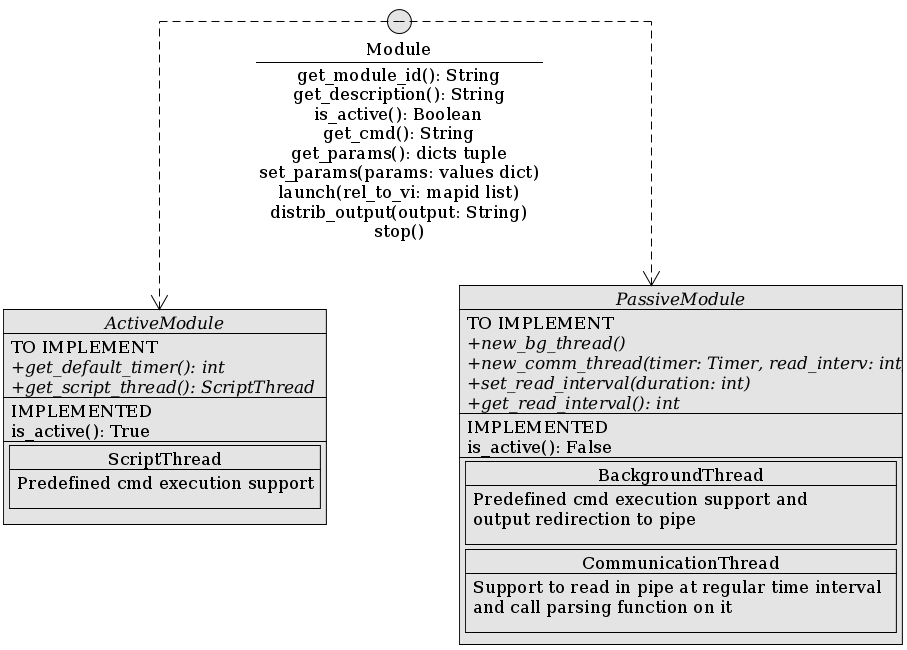
\includegraphics[width=0.585\textwidth]{abstrmodel.png}}
       \caption{Structure orientée objet du modèle d'abstraction}
       \label{abstrmodeldiag}
    \end{figure}

\newpage

À noter que chaque module devrait garder une référence vers les threads dans lesquels il a lancé une exécution de son programme sous-jacent (plus de détails aux points suivants).
Les méthodes remarquables de l'interface \textit{Module} ont la sémantique suivante :
\vspace{0.1cm}
\begin{itemize}
\item[$\bullet$] \textit{get\_cmd()} : retourne l'alias qui sert à appeler le programme en CLI (comme lors d'une utilisation normale)
\item[$\bullet$] \textit{get\_params()} : obtention de 3 éléments : paramètres actuels, par défaut et leur description textuelle  
\item[$\bullet$] \textit{set\_params()} : ajustement de quels paramètres et de leur valeur à fournir à une exécution du programme
\vspace{0.2cm}
\item[$\bullet$] \textit{launch()} : lance une exécution du programme dans un nouveau thread, considérant les paramètres courants du Module. Des facilités pour un schéma d'exécution classique sont déjà implémentées dans les classes abstraites de l'archétype correspondant (ce sont des objets instanciables avec certains paramètres).
\vspace{0.1cm}
\item[$\bullet$] \textit{distrib\_output()} : méthode de parsing appelée sur la sortie textuelle de l'exécution d'un programme, effectue le travail de traduction vers les éléments de l'application
\vspace{0.1cm}
\item[$\bullet$] \textit{stop()} : interrompt l'exécution de tous les programmes sous-jacents dans les threads liés à l'instance du Module
\end{itemize}
    
\subsubsection{Design pour un module actif}

Le schéma d'exécution classique pour l'archétype actif est simple : l'appel à \textit{launch()} doit lancer l'exécution du programme sous-jacent avec les paramètres actuels du Module et dans un nouveau thread, auquel une fonction de callback (\textit{distrib\_output()}) est passée en paramètre. À la fin de l'exécution, la sortie du programme est récupérée et l'appel à la fonction de callback est effectué sur cette sortie (donc le parsing se fait dans la fin du fil d'exécution du thread). Ce comportement peut être obtenu grâce au support déjà implémenté dans la classe abstraite \textit{ActiveModule} dont un Module concret actif doit hériter. Il reste cependant des méthodes spécifiques au Module qui doivent y être implémentées (notamment celles de l'interface \textit{Module}). La \wordlink{abstractif}{figure} résume cette information.

    \begin{figure}[!h]
       \noindent\makebox[\textwidth]{%
       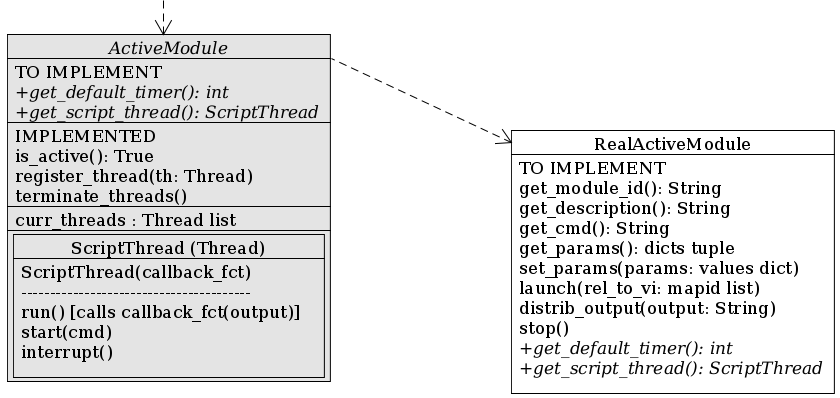
\includegraphics[width=0.73\textwidth]{abstractif.png}}
       \caption{Framework d'écriture d'un module actif}
       \label{abstractif}
    \end{figure}

\vspace{0.3cm}

\par Le code d'un Module actif devrait être structuré de la sorte :

\begin{enumerate}
\item \textit{get\_script\_thread()} doit retourner une instance de ScriptThread paramétrisée avec la fonction \textit{distrib\_output()} propre au Module.
\vspace{0.1cm}
\item \textit{launch()} construit la commande d'appel au programme \textit{cmd} depuis le schéma de paramètres et les paramètres actuels du Module, telle qu'elle serait invoquée en ligne de commande (en utilisant \textit{get\_cmd()} + les paramètres actuels dans \textit{get\_params()}).
\vspace{0.01cm}
\item \textit{launch()} instancie le conteneur de l'exécution avec \textit{get\_script\_thread()} et invoque sa méthode \textit{start()} avec \textit{cmd}, ce qui va lancer un nouveau thread dans lequel le processus du programme sous-jacent est créé. À la fin de son travail (\textit{run()} est bloquant dessus), la méthode \textit{distrib\_output()} est appelée sur sa sortie.
\vspace{0.1cm}
\item \textit{launch()}, après avoir créé et dissocié le thread du fil d'exécution, l'enregistre dans l'ensemble des exécutions courantes de l'instance du Module avec \textit{register\_thread()}.

\end{enumerate}
\vspace{0.2cm}
Additionnellement, la méthode \textit{get\_default\_timer()} renseigne la valeur par défaut que devrait prendre le timer d'expiration d'une instance du Module placée dans la Queue.

\newpage

\subsubsection{Design pour un module passif}

Pour un programme correspondant à l'archétype passif, le schéma d'exécution est complexifié car il faut pouvoir récupérer les sorties du programme au fur et à mesure qu'elles sont produites et de façon régulière. Effectivement, on ne peut pas attendre la terminaison du programme qui marque le fait qu'il y a quelque chose à lire sur sa sortie puisqu'il n'est pas censé terminer son exécution de lui-même. La solution choisie est de séparer le schéma d'exécution en deux parties. L'une contrôle le processus sous-jacent et redirige sa sortie vers un pipe temporaire pendant que l'autre partie y lit les sorties à intervalle régulier et les parse. Comme pour l'archétype actif, des facilités sont fournies pour gérer ce travail, illustrées par la \wordlink{abstrpassif}{figure}.

    \begin{figure}[!h]
       \noindent\makebox[\textwidth]{%
       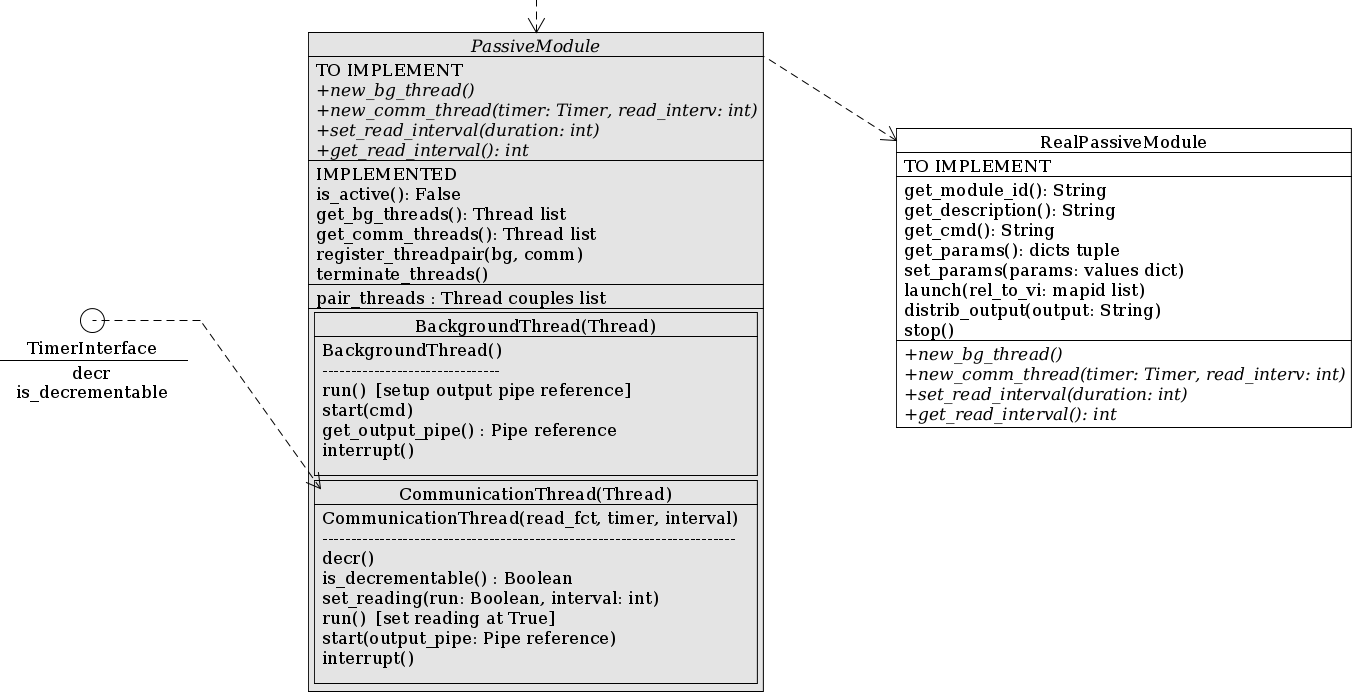
\includegraphics[width=0.9\textwidth]{abstrpassif.png}}
       \caption{Framework d'écriture d'un module passif}
       \label{abstrpassif}
    \end{figure}

Pour utiliser correctement ces facilités, l'implémentation du Module devrait respecter ces principes :
\begin{enumerate}
\item \textit{new\_bg\_thread()} et \textit{new\_com\_thread()} retournent respectivement une instance de BackgroundThread et CommunicationThread. Cette dernière doit être paramétrisée avec un objet Timer, l'intervalle de temps auquel la lecture doit avoir lieu et la fonction de parsing \textit{distrib\_output()} appelée sur la sortie lue
\vspace{0.2cm}
\item \textit{set\_read\_interval()} et \textit{get\_read\_interval()} sont relatifs à l'intervalle entre deux lectures qui doit être $> 0$
\vspace{0.2cm}
\item Comme pour les modules actifs, \textit{launch()} devrait construire la commande \texttt{cmd} telle qu'utilisable en CLI
\vspace{0.2cm}
\item Dans un premier temps, \textit{launch()} appelle la méthode \textit{start()} d'une instance de BackgroundThread en lui passant \texttt{cmd} pour démarrer le processus du programme sous-jacent, tout en redirigeant sa sortie vers un pipe alors créé à cette fin (\texttt{output\_pipe}). Une référence vers ce dernier est maintenue.
\vspace{0.2cm}
\item En second lieu, \textit{launch()} devrait attendre que le processus ait terminé son initialisation, c'est-à-dire que \texttt{output\_pipe} soit créé et accessible en lecture. Alors le CommunicationThread peut être instancié en le lui passant en paramètre.
\vspace{0.2cm}
\item Finalement, \textit{launch()} devrait enregistrer cette paire d'objets Thread dans la liste prévue à cet effet avec un appel à \textit{register\_thread\_pair()}
\end{enumerate}

\vspace{0.2cm}

À noter qu'ici, la méthode de BackgroundThread \textit{run()} lançant le sous-processus ne bloque pas jusqu'à sa terminaison (ce serait un perte de ressources). Également, la méthode \textit{run()} de CommunicationThread fait passer l'état de l'objet à \textit{décrémentable} puis termine le fil d'exécution du thread. C'est quand son timer tombe à 0 qu'un nouveau "dumb thread" est créé avec pour unique tâche de faire la lecture et le parsing. Cela se justifie par le fait que la méthode qui fait l'appel à la décrémentation (propre à l'objet Timer régissant l'application) ne devrait pas effectuer ce travail. En effet, il pourrait perturber la gestion de l'écoulement du temps s'il est trop lourd et effectué dans le même fil d'exécution. 
\newpage

\section{Implémentation de l'application}

%---------------- Choix

\subsection{Justification des choix généraux}

Comme l'application aspire à être déployée dans un environnement domestique, deux contraintes principales sont à prendre en compte pour son développement. La première est relative à l'utilisateur, qui de fait n'est pas une personne ayant une prédisposition particulière pour l'informatique. Un minimum de connaissances est quand même supposé : quelles sont les caractéristiques possibles d'un équipement sur le réseau, une idée de ce qu'est un scanneur de réseau, de ce que sont la prise d'empreintes et l'analyse de trafic, etc. L'interface doit être assez simple pour pouvoir manipuler les Modules et avoir une vue d'ensemble du réseau. La seconde contrainte concerne l'environnement restreint. Idéalement, l'application doit être fonctionnelle sur un équipement tel qu'une carte Raspberry PI, sans que l'interactivité avec en soit impactée. De plus, une utilisation dans un environnement non-graphique doit être possible, ce qui offrirait la possibilité de manipuler l'application à distance par le réseau, en utilisant \textit{ssh} par exemple. Ce dernier point va de pair avec une utilisation sur une carte Raspberry qui est contrôlée à distance.\\

\par Afin de concilier ces deux contraintes, la première interface développée est en ligne de commande. Elle se divise en deux parties : l'interaction (CLI) qui se présente comme des menus contextuels et la vue où l'état actuel de l'application est affiché clairement. L'utilisateur n'interagit qu'avec la première, qui lui permet de contrôler l'application en arrière-plan et la vue. L'application se lance depuis un terminal avec possibilité de lui passer certains arguments, puis utilise ce terminal comme CLI pour afficher le contenu des menus et récupérer les commandes que l'utilisateur y écrit afin de les interpréter. La vue est quant a elle initialisée après le cœur logique de l'application et peut se présenter sous plusieurs formes  en fonction des besoins de visualisation :
\vspace{0.2cm}
\begin{itemize}
\item[$\bullet$] \textbf{NoOutput} : aucune facilité n'est mise à disposition. Pour visualiser l'état actuel d'un élément de l'application, cela se fait via un menu \textit{show} qui affiche la cible dans la CLI même.
\vspace{0.2cm}
\item[$\bullet$] \textbf{PipeOutput} : l'élément cible à afficher ne l'est pas réellement, cette information textuelle est redirigée vers un pipe utilisable librement par l'utilisateur
\vspace{0.2cm}
\item[$\bullet$] \textbf{ConsoleOutput} : apporte un support de visualisation à PipeOutput, invoquant un nouveau terminal du système qui va maintenir un affichage de l'information envoyée dans le pipe (il ne sert qu'à cela)
\end{itemize}
\vspace{0.2cm}

\par La CLI permet de sélectionner ce qui doit être affiché dans la vue, et avec quel degré de détail. Il peut s'agir de la vue d'ensemble de l'application, du statut courant d'un Module dans la Queue et ses paramètres, etc. À titre d'exemple représentatif, la \wordlink{cli}{figure} montre ce à quoi ressemble l'interface et le système de menus.

\begin{figure}[!ht]
\centering
     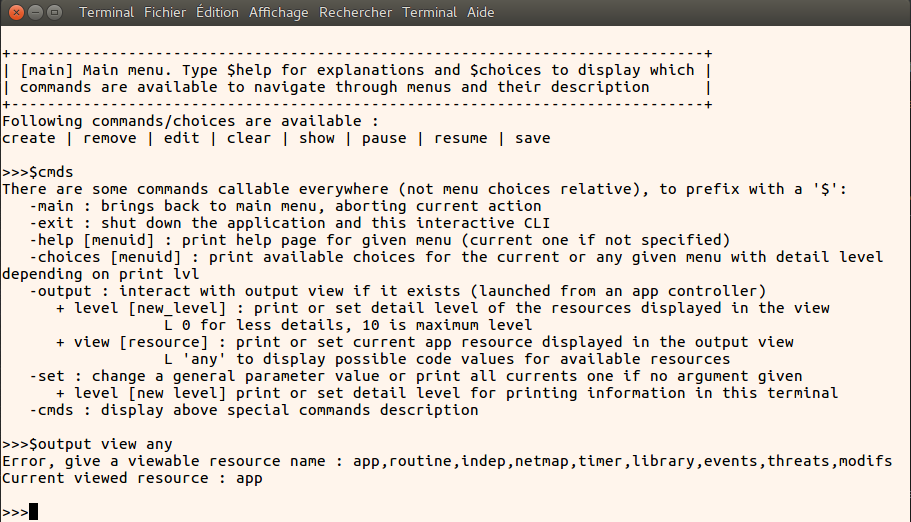
\includegraphics[width=0.7\linewidth]{clicmds}
     \caption{Interface CLI en mode ConsoleOutput}
     \label{cli}
\end{figure}

\par L'utilisateur peut entrer une valeur parmi les choix proposés, qui dépendent du menu actuel. Certaines commandes spéciales sont également invocables indépendamment, toutes préfixées par '\$'. Notamment la commande \texttt{\$output} qui permet de contrôler la vue, modifiant l'affichage courant.


\newpage
%---------------- Discussion implem

\subsection{Discussions des choix d'implémentation}

\subsubsection{Choix du langage}

Le langage qui a été sélectionné pour implémenter le cœur de l'application est le Python dans sa dernière version stable (3.7). La première interface développée n'étant pas graphique, elle est également réalisée en Python. L'application ne demandant en soit aucune opération ou algorithme à forte complexité, un langage compilé n'apporterait pas d'amélioration significative en terme de performances par rapport au Python. En effet, les seules opérations potentiellement lourdes seraient celles effectuées par certains programmes sous-jacents aux Modules, mais c'est alors indépendant du langage choisi. Cependant, l'expérience de l'utilisateur n'en sera pas directement impactée, car de par le design choisi chacune de ces exécutions a lieu dans un fil dissocié de l'exécution principale.\\

\par Python possède également une librairie standard assez vaste que pour couvrir à peu près tous les besoins de l'application (voir détails des points suivants). Comme une interface complète en ligne de commande est un objectif en terme d'interactivité avec l'utilisateur, la manipulation simplifiée des flux standards et un formatage aisé des chaînes de caractères sont des atouts importants de Python.

\subsubsection{Gestion du temps}

\noindent Librairie utilisée : \href{https://docs.python.org/3/library/time.html}{\texttt{time}}\\

\par Le temps intervient dans la gestion de plusieurs éléments de l'application : timers d'expirations des Modules actifs, lecture de la sortie à intervalle de temps donné pour les Modules passifs, mise à jour de la vue. Cette multiplicité a motivé le choix de créer un objet gestionnaire du temps unique et global a l'application. Les autres éléments de l'application nécessitant une interactivité temporelle s'enregistrent auprès de cet objet \textbf{TimerThread} et doivent implémenter une interface \textbf{\textit{TimerInterface}}. Cette interface ne contient que deux méthodes : \textit{decr()} qui est l'action à effectuer chaque seconde et \textit{is\_decrementable()} qui renvoie un booléen à vrai si \textit{decr()} doit être appelée.\\

Comme son nom l'indique, TimerThread va effectuer la gestion du temps dans un thread à part. Grâce aux primitives de la librairie \texttt{time}, le thread se réveille toute les secondes pour notifier tous les objets qui se sont enregistrés, c-à-d appelle la méthode \textit{decr()} de chacun individuellement si \textit{is\_decrementable()} de l'objet retourne vrai. L'action qui est ainsi effectuée par chacun des objets enregistrés est arbitraire et est spécifique à l'implémentation qui en est faite dans l'objet.

\subsubsection{Exécution des programmes sous-jacents}

\noindent Librairie utilisée : \href{https://docs.python.org/fr/3/library/subprocess.html}{\texttt{subprocess}}\\

\par La librairie standard de Python permet la manipulation aisée de processus tiers sous forme d'objet. Le seul prérequis est le passage de la commande système destinée à appeler le programme, telle qu'elle serait utilisée en ligne de commande. Il est également possible de fournir et d'en récupérer les flux d'entrées et sorties standards. Ces facilités sont exploitées dans l'implémentation du schéma d'exécution pour les Modules actifs et passifs. 

\subsubsection{Parsing des sorties}

Comme les sorties des programmes sous-jacents sont spécifiques et hétérogènes, leur traduction vers les éléments de l'application n'est pas gérée automatiquement. C'est au programmeur qui intègre le module d'écrire le code dédié à cette tâche. Cependant, des facilités sont envisageables pour cela. Actuellement, c'est le cas pour les sorties XML du programme Nmap : comme elles sont régies par une structure claire et définie quelqu'en soit l'utilisation, un parseur générique peut être fourni. Ce parseur peut être utilisé pour obtenir facilement des informations d'une sortie quelconque de Nmap et les manipuler comme des objets (correspondants à des \textit{elements} dans le DOM\footnote{\url{https://fr.wikipedia.org/wiki/Document_Object_Model}}).

\newpage

\subsubsection{Stockage et agrégation des informations}
\label{appcfg}
\noindent Librairie utilisée : \href{https://lxml.de}{\texttt{lxml}} (non intégré dans la librairie standard)\\

L'application maintient la Netmap, Routine, Librairie, etc. comme des objets, mais il est souhaitable que cette information soit retenue d'une exécution à l'autre et manipulable comme des fichiers indépendants. Considérant la quantité d'informations à stocker et la nature de conteneur de ces éléments, le choix à été fait d'utiliser le langage balisé XML. Des méthodes de traduction ont donc été écrites pour les deux sens : des éléments de l'application vers une représentation XML et inversement. Cela a été fait pour les éléments suivants : Modules, Librairie, Routine, Netmap, Events. En terme de fichiers XML individuels, on en retrouve un pour la Librairie, un pour la Routine et un dernier pour la Netmap qui renseignent donc toute l'information des objets qu'ils contiennent :\\

\begin{itemize}
\item[$\bullet$] XML de la Librairie : une entrée (ie. un \textit{element} pour le DOM) par module qui y est décrit, cette entrée contient des informations telles que l'id du module, le chemin du module python où est écrit la classe de l'objet Module, le nom de cette classe.
\vspace{0.2cm}
\item[$\bullet$] XML de la Routine : divisé en deux parties pour le Panel et la Queue, remplie chacune d'entrées représentant les Modules qui les peuplent. Chaque entrée renseigne l'id du module, son \texttt{setid} et ses paramètres courants au moment de la sauvegarde. Ces informations sont suffisantes pour réinstancier le Module à partir de la Librairie.\\

\item[$\bullet$] XML de la Netmap : stocke une entrée par Instance Virtuelle, avec toutes les informations littérales qui lui étaient associées. Les Events liés à chaque IV spécifique sont également écrits pour ne pas être perdus. 
\end{itemize}
\vspace{0.2cm}

\par Pour une exécution de l'application, on a donc trois fichiers principaux qui doivent être écrits si une sauvegarde permanente en est souhaitée, et parsés au relancement. Il y a également d'autres informations diverses qui peuvent être stockées comme l'adresse mail de l'utilisateur. Afin de regrouper cette information (notamment les chemins des fichiers XML), un super-fichier de configuration globale de l'application est nécessaire. Pour manipuler les chemins de sauvegardes et ces configurations suite à des changements de préférences par l'utilisateur lors de l'exécution de l'application, un objet \textbf{CoreConfig} est utilisé.\\

\par Le cœur logique de l'application ne prend qu'un seul paramètre à son initialisation qui doit être une instance de CoreConfig, ce qui permet de séparer le chargement des ressources et leur instanciation de leur utilisation. Une instance de CoreConfig peut être créée en parsant le super-fichier de configuration, qui est un fichier au format YAML et contient notamment les chemins des autres fichiers XML cités précédemment. Les différents fichiers sont alors parsés et les objets correspondant instanciés dans un ordre prédéfini car il y a des dépendances entre eux. Si des chemins sont inexistants dans le fichier de configuration, les éléments sont instanciés vides et avec leurs paramètres par défaut. Plusieurs fichiers de configurations coexistant sont envisageables, par exemple si l'utilisateur souhaite utiliser des routines différentes en fonction du réseau dans lequel il lance l'application. La seule contrainte étant qu'à un lancement d'application un seul fichier de configuration soit passé et potentiellement modifiable durant l'exécution.

\subsubsection{Interactivité avec l'application}
\label{justifinter}

Le système de menus interactifs a été conçu dans l'optique d'être utilisable simplement par une personne non initiée. Aucune librairie tierce n'a été utilisée pour le mettre en place, excepté les méthodes Python natives de prises d'entrées et complétion. Brièvement, un menu est représenté en interne par un dictionnaire dont plusieurs valeurs associés à des clés spécifiques doivent être définies. On y retrouve notamment :\\
\begin{itemize}
\item[$\bullet$] \texttt{desc} : une description textuelle du menu, quelle est sa fonction par rapport aux choix qu'il propose
\vspace{0.1cm}
\item[$\bullet$] \texttt{choices} : une liste de choix qui peut être sous plusieurs forme (liste, dictionnaire, fonction qui retourne un des deux) qui sont les entrées possibles pour le menu courant
\vspace{0.1cm}
\item[$\bullet$] \texttt{fct\_choice} : une fonction dite de choix prenant une valeur en argument (qui sera le choix entré)
\end{itemize}
\vspace{0.2cm}

Une procédure bouclant sans fin permet de naviguer à travers les menus. Le menu courant correspond à un dictionnaire définissant les champs cités ci-dessus. Les choix disponibles sont calculés et mis en forme pour être présentés à l'utilisateur dont l'entrée est attendue. Une fois qu'il a fourni une entrée correcte, la fonction de choix est appelée sur cette entrée dont dépendent alors les actions effectuées. Par exemple, la fonction de transition de menu va simplement remplacer le menu courant par celui auquel correspond l'entrée de l'utilisateur, ce après quoi la procédure reprend du début.

\subsubsection{Alertes et notifications par email}

\noindent Librairies utilisées : \href{https://docs.python.org/3/howto/logging.html}{logging} et \href{https://docs.python.org/3/library/smtplib.html}{\texttt{smtplib}}\\

\par L'utilisateur doit pouvoir être alerté efficacement quand une menace est détectée par un Module. En l'occurrence, cette information doit être observable et récupérable depuis l'interface, mais également communiquée à l'utilisateur autrement puisqu'il n'est pas forcément présent devant l'interface. L'option la plus évidente est de notifier les menaces considérées comme importantes par mail. À cette fin, l'utilisateur peut fournir son adresse mail à l'application. Pour éviter des complications et la configuration d'un serveur dédié, le compte mail utilisé pour envoyer les notifications est celui de l'utilisateur lui-même. Il lui sera donc demandé son mot de passe afin de se connecter au serveur authentifié SMTP dont il utilise les services.\\

\par D'un point de vue implémentation, le lancement des alertes et la remontée des informations vers le centre d’événements de l'application depuis le code d'un Module doit être aisé. On distingue quatre façons de faire parvenir de l'information à l'utilisateur :
\begin{enumerate}
\item Par logging classique (utilisation des fonctionnalités natives de \texttt{logging}) avec les loggers \texttt{debug, info, error, cli, threats, modifs} qui redirigent l'information vers les flux d'entrées standards et les fichiers de logs.
\vspace{0.1cm}
\item En créant des objets Events qui seront gardés en mémoire dans l'application pour être manipulés. Facilité de programmation fournie : chaque objet Logger accessible classiquement en important \texttt{logging} (voir ci-dessus) est agrémenté d'une méthode \textit{register\_threat()}/\textit{register\_modif()} qui instancie cet Event, le garde en mémoire et le log de façon régulière en fonction du Logger concerné.
\vspace{0.1cm}
\item En enregistrant une entrée dans la zone de feedback de l'application, qui est un historique court affiché à l'utilisateur dans la vue (simples chaînes de caractères d'information). La méthode \textit{log\_feedback()} agrémente le module \texttt{logging} à cet effet et permet également de logger de façon régulière l'information par un Logger désigné.
\vspace{0.1cm}
\item En envoyant un mail contenant un message personnalisé à l'utilisateur s'il a fourni une adresse. Cela se fait classiquement via le Logger \texttt{mail}. 
\end{enumerate}
\vspace{0.1cm}

Le module python \texttt{logging} a comme particularité de pouvoir être importé n'importe où dans le code mais de permettre l'accès aux même instances de Logger par un identifiant unique. Cela permet d'éviter de devoir transporter des références vers ceux-ci à travers le code. On peut donc utiliser cela et y coupler d'autres facilités personnalisées, en déclarant des nouvelles méthodes pour ces objets : \textit{register\_threat()}/\textit{register\_modif()} et \textit{log\_feedback()}.\\

\par De base, \texttt{logging} gère l'envoi de mail. Cependant, ce n'est pas le cas pour le SMTP authentifié qui est utilisé majoritairement. La librairie standard \texttt{smtplib} permet de pallier à ce problème en sous-classant l'utilitaire de base de \texttt{logging}.

%---------------- Logiciels


\newpage

\section{Manuel d'utilisation}
\label{manuel}

\subsection{Prérequis et installation}
\label{install}
Les prérequis généraux sont :
\begin{itemize}
\vspace{0.1cm}
\item[$\bullet$] Une distribution Linux (testé sous Debian, Ubuntu, Arch)
\vspace{0.1cm}
\item[$\bullet$] Les programmes sous-jacents installés et invocables depuis un shell (si ce n'est pas le cas une option permet de tenter l'installation automatique des programmes manquants)
\vspace{0.1cm}
\item[$\bullet$] Une version de Python $\geq 3.7$
\vspace{0.1cm}
\item[$\bullet$] Les droits de super-utilisateur pour lancer l'application
\end{itemize}
\vspace{0.1cm}

Au niveau librairies, quelques dépendances doivent être installées si non présentes par défaut. Cela peut se faire avec la commande suivante :\\

\indent \texttt{sudo apt-get install python-yaml python3-lxml libxml2-dev libxslt1-dev xterm}
\vspace{0.4cm}

\par Ensuite, une fois en possession des sources du projet (\texttt{git clone \url{https://github.com/RemDec/IoTMonitor}}), les dépendances aux librairies python et l'initialisation des fichiers requis peuvent être gérés en appelant à la racine~\\

\indent \texttt{python3.7 setup.py develop}
\vspace{0.4cm}

\par On distingue deux types d'utilisateurs qui sont susceptibles d'utiliser l'application, dans une optique différente. On a d'une part les utilisateurs normaux qui se servent de l'application pour son but premier : protéger leur réseau domestique. Leurs interactions se font uniquement depuis l'interface et avec les Modules fournis. D'autre part, on a des personnes avec des connaissances plus avancées en programmation, capable d'assimiler le framework mis à disposition et intéressées par son utilisation. Ces dernières souhaitent intégrer leurs propres outils (sous-entendu programmes) pour pouvoir les manipuler dans l'application, et ont donc besoin d'une marche à suivre pour arriver à cette fin. Les deux cas d'utilisation sont distingués dans les sections suivantes qui font office de guide.

\subsection{Utilisation classique}

\subsubsection{Point d'entrée de l'application}

À la racine du projet se trouve le point d'entrée en ligne de commande de l'application \texttt{IoTMonitor.py}. Plusieurs arguments peuvent lui être passés, mais ils sont tous optionnels (l'application sera lancée avec des paramètres par défaut). En revanche, il est nécessaire d'invoquer la commande avec les droits de super-utilisateur et en utilisant une version de Python $\geq 3.7$. Une page d'aide est affichable avec le flag \texttt{-h}. Quelques autres paramètres sont utiles :\\
\begin{itemize}
\item[$\bullet$] \texttt{--fileconfig FILEPATH} : indique le super-fichier de configuration tel que décrit au \wordlink{appcfg}{point}.
\vspace{0.2cm}
\item[$\bullet$] \texttt{--noautosave} : par défaut, quand l'application est quittée, l'état actuel des éléments est sauvegardé de sorte qu'au prochain lancement, leur état est restauré. Ce flag désactive cette fonctionnalité.
\vspace{0.2cm}
\item[$\bullet$] \texttt{--noautoload} : par défaut, au lancement de l'application, l'état des éléments est restauré à celui qu'il était quand elle a été quittée (vierge si \texttt{noautosave} était mis). Désactive cette fonctionnalité, permettant de partir d'éléments vierges (routine, etc.).
\vspace{0.2cm}
\item[$\bullet$] \texttt{--mail MAIL} : renseigne l'adresse mail de l'utilisateur que l'application utilisera pour les notifications d'alertes. Préférentiellement à utiliser avec le flag \texttt{--testmail} qui testera la validité et accessibilité de cette adresse en envoyant un email témoin.
\vspace{0.2cm}
\item[$\bullet$] \texttt{--installprogs} : tente d'installer tous les programmes sous-jacents aux Modules qui ne le sont pas encore sur le système (en utilisant divers gestionnaires de paquets)
\end{itemize}
\vspace{0.2cm}

\par Si une adresse mail est renseignée, le mot de passe pour le serveur SMTP authentifié le sera également, les mails étant envoyés à l'utilisateur avec sa propre adresse. Quand une menace est détectée par un Module, celui-ci est susceptible d'en alerter l'utilisateur. Si aucune adresse mail n'est spécifiée, aucune tentative d'émission de mail n'aura lieu.\\

\newpage

\par Pour lancer l'application dans une configuration recommandée pour débuter, la commande suivante peut être utilisée :
\begin{center}
\texttt{sudo python3.7 IoTmonitor.py -nal --mail untel@gmail.com --mserver smtp.gmail.com --testmail}
\end{center} 

Fournir le serveur SMTP n'est pas obligatoire, mais conseillé car sinon il sera deviné et donc peut être erroné. Cette commande va lancer l'application en mode ConsoleOutput, invoquant un nouveau terminal (xterm par défaut) qui servira de vue sur son état actuel. Le terminal depuis lequel elle est invoquée sera celui dans lequel les entrées de l'utilisateur sont récupérées. Deux remarques à prendre en compte pour cette étape :

\begin{enumerate}
\item Certain fournisseurs de services mail (Gmail par exemple) peuvent demander des autorisations supplémentaires. Voir les remarques dans la fiche d'aide avec \texttt{-h}.
\vspace{0.2cm}
\item Pour éviter certains bugs graphiques, il est préférable de lancer cette commande dans un terminal assez grand en terme de taille par rapport au reste de l'écran, voire en plein écran.
\end{enumerate}

\subsubsection{Navigation dans les menus}

Une fois lancée, l'application initialise sa partie logique et l'utilisateur se retrouve dans la partie interactive, dont le point de départ est le menu principal. La combinaison de la vue et de l'interface devrait être similaire à celle illustrée dans la \wordlink{startapp}{figure}. Les conteneurs principaux, la Netmap et la Routine, y sont illustrés comme vides.

\begin{figure}[!ht]
   \begin{adjustwidth}{-\oddsidemargin-1in + 0.5cm}{-\rightmargin}
     \centering
     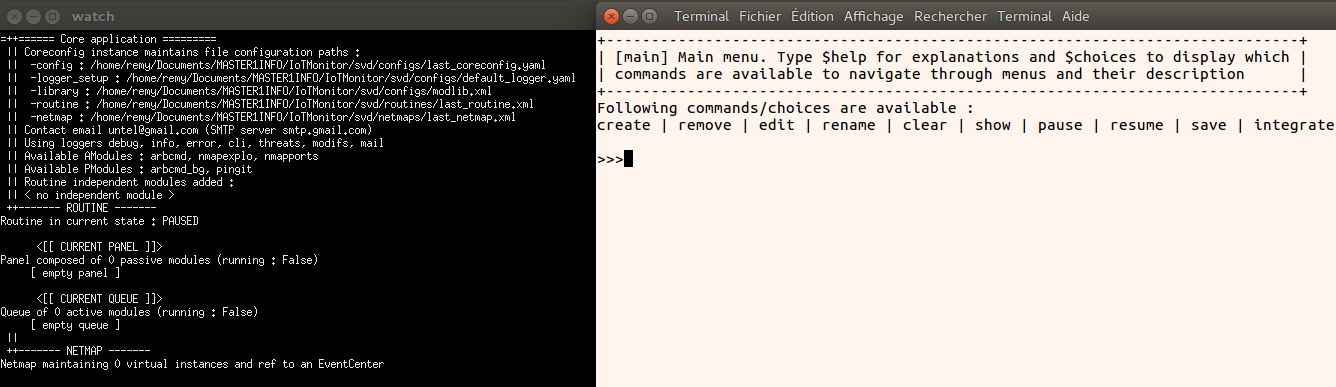
\includegraphics[width=\paperwidth - 1cm]{startapp}
     \caption{Application au démarrage (fenêtre de vue et CLI)}
     \label{startapp}
   \end{adjustwidth}
   \
\end{figure}

Un cadre surplombant le champ de prise d'entrées renseigne quel est l'id du menu courant et une courte description de son utilité. Juste en dessous sont affichés les choix possibles pour ce menu, c'est-à-dire ce que l'utilisateur peut entrer comme valeur. Un système d'autocomplétion classique (touche \texttt{<Tabulation>}) permet de sélectionner rapidement un choix parmi ceux possibles, à valider par la touche entrée. De plus, appuyer sur entrée en n'ayant tapé que le début du mot le sélectionne automatiquement s'il n'y a aucune ambiguïté avec ce choix. Indépendamment du menu courant, des commandes spéciales sont invocables pour effectuer diverses actions, toutes à préfixer par le symbole '\$'. La liste de ces commandes est explicitée en tapant \texttt{\$cmds}.\\

\par Le menu principal permet d'accéder à tous les autres menus en naviguant de choix en choix. Un appel à \texttt{\$choices} permet d'en savoir plus sur ces menus associés chacun à un choix, comme illustré par la \wordlink{choicesmain}{figure}. Pour revenir au menu principal depuis un menu quelconque, la commande \texttt{\$main} peut être utilisée.

\begin{figure}[!ht]
\centering
     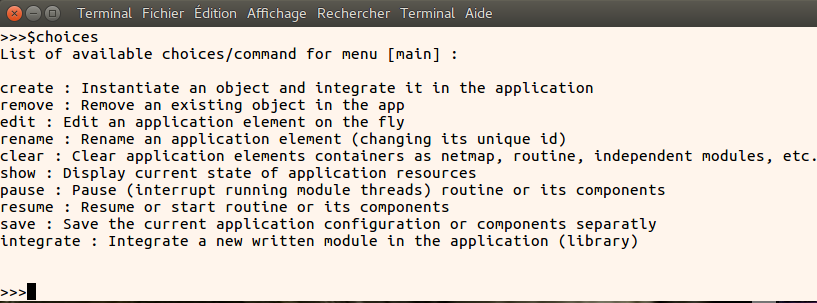
\includegraphics[width=0.65\linewidth]{choicesmain}
     \caption{Description des sous-menus accessibles depuis le menu principal}
     \label{choicesmain}
\end{figure}

\newpage

\subsubsection{Consultation de l'état des éléments}

Bien que ce qui est affiché dans la vue soit contrôlable en utilisant la commande \texttt{\$output}, il est parfois plus utile et précis d'afficher le statut de l'élément désiré dans le terminal de l'interface même. Cela peut se faire en se rendant dans le menu \texttt{show} accessible depuis le menu principal. Un panel d'éléments dont les détails sont consultables est proposé à l'utilisateur. La navigation dans plusieurs menus contextuels consécutifs peut être nécessaire pour spécifier l'élément visé : par exemple pour une Instance Virtuelle précise, il sera demandé d'entrer le mapid correspondant.\\

\par Lors de l'affichage de l'information désirée, un paramètre déterminant le niveau de détail est pris en compte. Pour modifier cette valeur avant l'affichage, la commande \texttt{set} peut être utilisée comme suit : \texttt{\$set lvl [niveau]} où niveau est un entier entre 0 et 10, mais la majeur partie des éléments peuvent fournir plus de détail jusqu'au niveau 5. Il en va de même avec l'élément affiché dans la vue, la configuration passant cette fois par la commande \texttt{\$output}.

\subsubsection{Exemple pratique d'utilisation}

Les actions rentrant en jeu pour mettre en place une surveillance du réseau domestique peuvent être réalisées aisément par n'importe quel utilisateur qui a compris les concepts de Modules et Routine. Cela peut se résumer à sélectionner quels Modules instancier dans la Librairie parmi ceux disponibles par défaut et à les ajouter à la Routine. La description des Modules, le travail qu'ils effectuent et les paramètres qu'ils prennent sont accessibles en affichant la Librairie. Cela se fait donc en accédant au menu \texttt{show} depuis le menu principal, puis en sélectionnant l'élément Librairie en tapant \texttt{library}. Une description similaire à la \wordlink{showlib}{figure} est affichée pour chaque Module disponible.

\begin{figure}[!ht]
\centering
     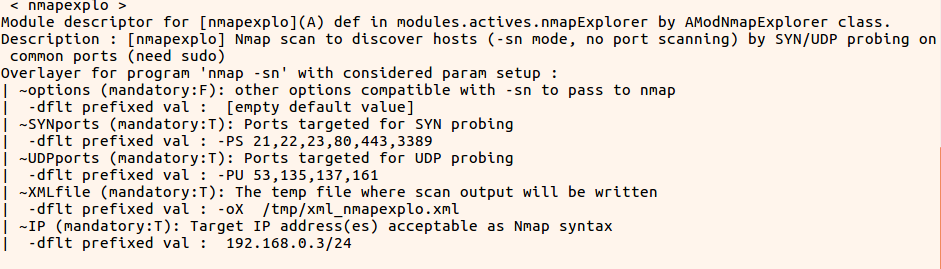
\includegraphics[width=0.9\linewidth]{showlib}
     \caption{Affichage de la description pour le module \texttt{nmapexplo}}
     \label{showlib}
\end{figure}

Cela renseigne que le programme sous-jacent est \textit{nmap} et est d'office utilisé avec l'option \textit{-sn} qui signifie "passer la phase de scan des ports". Effectivement, comme l'indique la description fournie, il s'agit d'un Module pour la découverte des hôtes uniquement. Viennent ensuite les paramètres qu'il peut prendre avec leur code, leur description textuelle et la valeur préfixée telle qu'elle sera insérée dans la ligne de commande appelant le programme. Un paramètre dit "mandatory" sera toujours présent dans cette ligne de commande et prendra la valeur par défaut associée si aucune autre n'est fournie. Les valeurs par défaut des paramètres optionnels (non "mandatory") ne sont donc juste là qu'à titre indicatif, car le paramètre sera ignoré si aucune valeur ne lui est manuellement fournie. À noter que certaines valeurs par défaut de paramètres peuvent être recalculées dynamiquement à l’instanciation du Module, comme l'IP dans ce cas (pour correspondre à celle du réseau local).\\

\par Une fois la sélection des Modules à utiliser terminée, il faut les instancier dans la Routine. Cela se fait en revenant au menu principal avec \texttt{\$main} et en choisissant le menu \texttt{create}. Le choix par défaut est indiqué par \texttt{$< . >$}, qui est bien ici sur \texttt{module}, on peut donc le sélectionner directement en appuyant sur Entrée. La liste des ids des modules disponibles dans la Librairie est affichée, en premier lieu les Modules passifs et à la ligne suivantes les actifs. Après avoir entré l'id voulu, une série de questions amenant à des sous-menus contextuels sont posées afin de configurer l'instance du Module et son comportement dans la Routine (\wordlink{newmod}{figure}) :\\
\begin{enumerate}
\item Utiliser les paramètres par défaut ?
	\begin{itemize}
	\item[$\bullet$] Si oui, le Module verra ses paramètres courants mis à leur valeur par défaut et aucun paramètre optionnel ne sera utilisé.
	\item[$\bullet$] Si non, pour chaque paramètre existant une valeur sera demandée, appuyer sur Entrée revenant à utiliser celle par défaut.
	\end{itemize}  
\vspace{0.2cm}
\item Ajouter l'instance dans la Routine ?
	\begin{itemize}
	\item[$\bullet$] Si oui, l'instance du Module sera ajoutée dans le conteneur correspondant à ton archétype (Panel ou Queue).
	\item[$\bullet$] Si non, l'instance est ajoutée à l'ensemble des Modules indépendants, où il sera exécuté une unique fois directement
	\end{itemize}
\vspace{0.2cm}
\item Fournir des Instances Virtuelles spécifiques auxquelles l'exécution du Module devrait se rapporter ?
	\begin{itemize}
	\item[$\bullet$] Si oui, un sous-menu permettra de donner les mapids des IVs concernées. Le Module pourra utiliser cette information à des fins diverses, vraisemblablement il exécutera son programme sous-jacent vis-à-vis de celles-ci mais cela dépend entièrement de son implémentation.
	\item[$\bullet$] Si non, le Module s'exécutera indifféremment où en considérant toutes les VIs s'il avait besoin de cibles données.
	\end{itemize}
\vspace{0.2cm}
\item Spécifier un timer ? (intervalle de lecture pour un Module passif ou timer d'expiration pour un actif)
	\begin{itemize}
	\item[$\bullet$] Si un entier est entré, utilisation de cet entier comme le nombre de secondes
	\item[$\bullet$] Si rien n'est spécifié, utilisation de la valeur par défaut
	\end{itemize}
\vspace{0.2cm}
\item Spécifier un \texttt{setid} à utiliser pour identifier l'instance du module dans la Routine ?
	\begin{itemize}
	\item[$\bullet$] Si une chaîne de caractères est entrée le \texttt{setid} sera mis à cette valeur
	\item[$\bullet$] Si rien n'est spécifié, utilisation de l'id du module
	\end{itemize}
\vspace{0.2cm}
\end{enumerate}

\begin{figure}[!ht]
\centering
     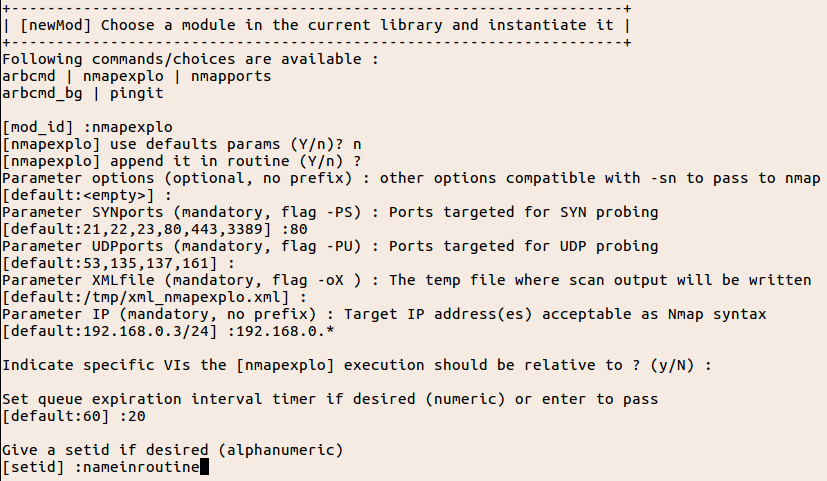
\includegraphics[width=0.8\linewidth]{newmod}
     \caption{Instanciation du module \texttt{nmapexplo} à placer dans la Routine}
     \label{newmod}
\end{figure}


Après remplissage de la Routine avec plusieurs instances de Modules différents, on peut observer son état dans la vue (\wordlink{vueroutine}{figure}). Pour chaque instance de Module, on a un résumé de son état actuel informant également du nombre de thread(s) courant(s) qui lui sont associés. Sur la \wordlink{vueroutine}{figure} on observe qu'aucun thread n'est enregistré donc aucun programme sous-jacent n'est en cours d'exécution. C'est normal car la Routine est toujours en état de pause. Pour lancer la Routine automatique de surveillance, le menu \texttt{resume} doit être accédé depuis le menu principal et \texttt{entire routine} doit y être choisi. 

\begin{figure}[!ht]
\centering
     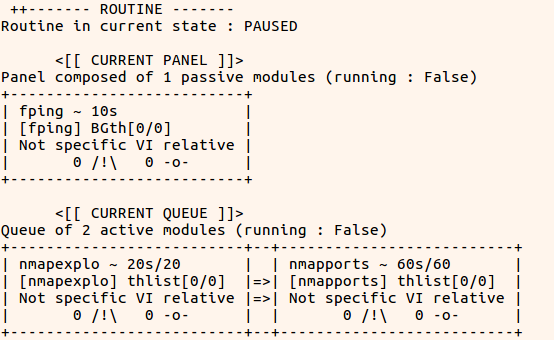
\includegraphics[width=0.7\linewidth]{vueroutine}
     \caption{État de la Routine après remplissage}
     \label{vueroutine}
\end{figure}

La Routine illustrée permet de découvrir et analyser les équipements du réseau domestique pour en regrouper les caractéristiques. La Netmap devrait donc se remplir au fur et à mesure des exécutions des Modules pour converger vers une représentation du réseau avec les différents équipements qui le peuplent. À titre d'exemple, la Netmap de la\wordlink{vuenetmap}{figure} est celle obtenue après un court moment.


\begin{figure}[!ht]
\centering
     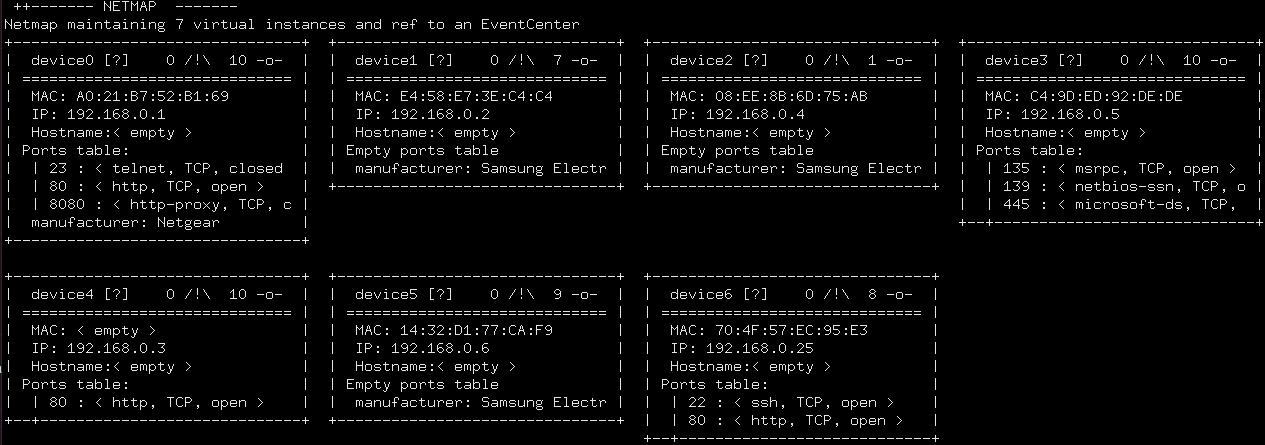
\includegraphics[width=\linewidth]{netmap}
     \caption{État de la Netmap après que la routine de la \wordlink{vueroutine}{figure} ait tourné un court moment}
     \label{vuenetmap}
\end{figure}

\par Cette représentation de la Netmap a pour but de donner une vue d'ensemble du réseau. Dans l'en-tête de chaque vignette d'IV, le symbole entre crochet représente l'état de connexion au réseau ('?' indique un flou), $n$ /!\textbackslash  indique le nombre de menaces trouvées pour l'équipement et $n$ -o- le nombre de modifications de ses champs. Pour consulter en détail ces informations, le choix \texttt{virtual instance} du menu \texttt{show} est utilisable.\\

\par Pour agrémenter et améliorer la représentation du réseau, l'utilisateur peut rentrer ou corriger lui-même les valeurs des champs d'une IV, voire la créer de toute pièce. Cela se fait via les menus \texttt{edit} et \texttt{create} respectivement. Il en va de même pour les instances de Module. D'autres menus gèrent des fonctionnalités diverses, tel que \texttt{save} qui permet d'écrire les fichiers de sauvegarde de la Routine et de la Netmap décrits au \wordlink{appcfg}{point}, ainsi de redéfinir les références vers les fichiers de sauvegardes à utiliser à l'initialisation (définies dans le super-fichier de configuration). 

\subsection{Utilisation du point de vue du programmeur}

\subsubsection{Écrire un module}
\label{writemod}

À un Module correspond, en terme de code, une classe astreinte à suivre le framework imposé. Par convention, le nom de celle-ci doit commencer par "AMod" pour un Module actif et "PMod" pour un Module passif. En fonction de l'archétype associable au programme sous-jacent à abstraire, cette classe doit également hériter de la classe abstraite correspondante : \textit{ActiveModule} ou \textit{PassiveModule}. De fait, elle devra également en implémenter les méthodes abstraites. Sans ces conditions, l'intégration d'un nouveau module à l'application ne se fera pas correctement.\\

\par Deux options sont possibles pour l'implémentation d'une classe correspondant à un nouveau Module. La plus simple des deux est aussi celle qui offre le moins de contrôle : il s'agit de deux sous-classes (abstraite également) à \textit{ActiveModule} et \textit{PassiveModule} implémentant l'utilisation des facilités fournies par ces dernières (voir \wordlink{abstrmodel}{sous-section}). Ces deux sous-classes sont respectivement \textit{FacilityActiveModule} et \textit{FacilityPassiveModule}. Elles implémentent le maximum de ce qui peut l'être en ne laissant comme abstraites que les méthodes spécifiques à chaque Module (i.e. liée avec le programme sous-jacent). L'autre option, qui nécessite plus de travail mais permet de personnaliser davantage le comportement d'un Module, est de simplement hériter de \textit{ActiveModule} ou \textit{PassiveModule} en implémentant toutes les méthodes abstraites. La possibilité d'utiliser les facilités fournies de ces deux classes est alors laissée comme libre (notamment la façon dont l'exécution est gérée).\\ 

Plus concrètement, les méthodes abstraites à implémenter dans une sous-classe de \textit{FacilityActiveModule} et \textit{FacilityPassiveModule} sont les suivantes :\\
\begin{itemize}
\item[$\bullet$] \textit{get\_module\_id(), get\_cmd(), get\_description()} qui sont des chaînes de caractères pour respectivement l'id unique du Module, la commande système utilisée pour appeler le programme en CLI et une description textuelle du Module
\vspace{0.2cm}
\item[$\bullet$] \textit{get\_scheme\_param()} qui sert à décrire quels paramètres le Module peut prendre et de quelle façon il sont traités : un dictionnaire dont les clés sont les noms des paramètres et les valeurs des triplets \textit{(valeur par défaut, obligatoire, préfixe en CLI)}
\vspace{0.2cm}
\item[$\bullet$] \textit{get\_desc\_params()} retourne un dictionnaire mappant chaque nom de paramètre avec une description textuelle de son utilité
\vspace{0.2cm}
\item[$\bullet$] \textit{build\_final\_cmd()} crée la commande telle qu'elle serait passée en CLI à partir de \textit{get\_cmd()}, les valeurs courantes des paramètres et le schéma de traitement de ces valeurs donné par \textit{get\_scheme\_param()}.
\vspace{0.2cm}
\item[$\bullet$] \textit{parse\_output(output)} est la méthode de parsing de la sortie du programme qui est censée faire la traduction vers des éléments du reste de l'application
\vspace{0.2cm}
\end{itemize}

Au final, implémenter un nouveau Module avec ces facilités revient à écrire une classe d'à peu près 150 lignes dont la moitié constituent la fonction de parsing des sorties, seul travail laborieux mais incontournable.\\

\par Afin de quand même faciliter le travail à effectuer pour l'implémentation en sous-classant directement \textit{ActiveModule} ou \textit{PassiveModule}, deux classes "squelette" types déjà structurées sont fournies. Il suffit d'en reprendre le code en y apportant les personnalisations voulues et les informations à remplir (id du Module, etc.).\\

\par Des facilités de logging et de création d'Events sont également utilisables. Elle permette de simplement déclarer de nouvelles modifications de valeurs des champs d'Instance Virtuelle, des menaces les concernant, envoyer un mail, etc. Pour rappel, plusieurs loggers sont présents de base à l'initialisation, avec des objectifs différents : afficher un message dans la CLI, enregistrer les événements importants dans des fichiers de logs y étant dédiés, et d'autres utilitaires.

\newpage

\subsubsection{Intégrer un module dans l'application}

Pour intégrer un nouveau Module à l'environnement afin qu'il y soit manipulable, il faut l'ajouter à la Librairie qui est chargée à l'initialisation. Cette libraire est représentée par un fichier XML unique dont le chemin est \texttt{svd/configs/modlib.xml}, celui-ci n'étant pas modifiable pour pointer vers un autre fichier. La Librairie est construite en le parsant, chaque entrée s'y trouvant représente un Module et ses informations. Afin de faire le lien avec le code python du Module, le nom du package et le nom du module python dans lequel la classe est écrite sont fournis dans les attributs XML de l'entrée. Un exemple d'entrée dans ce document est le suivant :
\small{
\lstset{language=XML}
\begin{lstlisting}
<actmod modid="nmapexplo" cmd="nmap -sn" pymod="modules.actives.nmapExplorer" pyclass="AModNmapExplorer">
  <desc>[nmapexplo] Nmap scan to discover hosts (-sn mode, no port scanning) by SYN/UDP probing ...</desc>
  <defparams>
    <param code="options" mandatory="False" default="" prefix="">other options compatible with -sn to ...</param>
    <param code="SYNports" mandatory="True" default="21,22,23,80,443,3389" prefix="-PS">Ports targeted for ...</param>
    <param code="UDPports" mandatory="True" default="53,135,137,161" prefix="-PU">Ports targeted for UDP ...</param>
    <param code="XMLfile" mandatory="True" default="/tmp/xml_nmapexplo.xml" prefix="-oX ">The temp ...</param>
    <param code="IP" mandatory="True" default="192.168.0.3/24" prefix="">Target IP address(es) acceptable ...</param>
  </defparams>
  <savedparams/>
  <dependencies/>
</actmod>
\end{lstlisting}
}

Trois options s'offrent au programmeur pour intégrer son module, qui sont par ordre de facilité :

\begin{enumerate}
\item Intégration via l'interface CLI (menu \texttt{integrate}) en fournissant le module python
\item Par programme, en instanciant un petit objet utilitaire ModuleIntegrator
\item Par écriture directe dans le fichier \texttt{modlib.xml}
\end{enumerate}

\par L'intégration par CLI fait l'hypothèse que le code décrivant l'objet Module se trouve au bon endroit dans les package pythons destinés à les regrouper par archétype \texttt{modules.passives} et \texttt{modules.actives}. Le code doit contenir une classe respectant les conditions évoquées au \wordlink{writemod}{point} et qui est le code du Module. Supposons que le fichier contenant le code s'appelle mymodule.py, alors celui-ci correspond au module python \texttt{mymodule} (dans l'arborescence \texttt{modules.passives.mymodule} ou \texttt{modules.actives.mymodule}). Arrivé dans le menu \texttt{integrate}, le programmeur renseigne l'archétype de son nouveau Module. Il lui est en suite demandé d'entrer le nom du module python dans lequel il est définit : en l'occurrence \texttt{mymodule}. Si toutes les conventions ont été respectées, une entrée devrait être écrite dans le fichier modlib.xml, celui-ci reparsé et le Module devrait apparaître parmi ceux disponibles.\\

\par L'objet utilitaire pour intégrer un Module à partir d'une de ses instances (donc créée par programme ou dans l'interpréteur Python) est trouvable dans le package \texttt{src.utils.filesManager}. Il s'agit de la classe \textbf{ModuleIntegrator}, qui prend en paramètre de constructeur une instance du Module à intégrer ou une chaîne de caractères désignant le module python à importer pour trouver la classe correspondante (\texttt{modules.passives.mymodule}). En instanciant un objet Library du module \texttt{src.utils.moduleManager}, il est également possible d'intégrer la nouvelle entrée au fichier grâce à la méthode \textit{add\_to\_modlib\_file(mod instance)}.\\

\par La troisième façon d'intégrer un Module nouvellement écrit est celle la moins recommandée. Il s'agit simplement d'écrire l'entrée XML manuellement. Cela devrait être fait dans le fichier qui est chargé d'office : \texttt{modlib.xml}.

\newpage


\section{Tests et évaluation de l'application}

\subsection{Déploiement sur Raspberry Pi et utilisation distante}

Afin de valider l'application dans l'environnement qu'on lui destinait, les prochains tests effectués  dans un réseau réel le sont sur une machine restreinte en ressources : une carte Rasperry Pi 3 (sous Raspbian installé). L'interaction avec cette dernière se fait à distance via ssh depuis une station assimilable à un PC banal. On utilisera donc dans ce cas le mode PipeOutput à la place du mode classique ConsoleOutput. Afin de visualiser le contenu de la Vue, il sera nécessaire de jouer avec un deuxième shell connecté via ssh au Raspberry et d'afficher le contenu du pipe créé.\\

Au préalable, Python 3.7 doit être installé manuellement\footnote{\url{https://github.com/instabot-py/instabot.py/wiki/Installing-Python-3.7-on-Raspberry-Pi}} (non fourni par Raspbian). Ce après quoi on applique les instructions d'installation données à la \wordlink{manuel}{section}. Ces opérations étant toutes réalisables via une connexion ssh existante, on suppose qu'il est possible d'en établir une seconde depuis un autre terminal (qui servira de Vue). Dans la première qui servira d'interface interactive on lance l'application avec :~\\

\indent \texttt{sudo python3.7 IoTmonitor.py -m outpiped}
\vspace{0.4cm}
\par Un pipe est alors créé automatiquement dans /tmp et alimenté toutes les secondes avec l'état actuel de l'application (ou la ressource ciblée dans le cadre de la vue). Pour observer ces modifications de façon continue, on peut alors utiliser la commande \texttt{watch} dans le second terminal :~\\

\indent \texttt{watch -t -n 0,5 cat /tmp/output\_monitor}
\vspace{0.4cm}

Dans les tests réels décrits ci-dessous, l'application a été utilisée sur ladite carte Raspberry de cette façon. Il est à noter que la consommation en terme de ressources n'y est pas mentionnée car elle se révèle très faible. On observe que le processeur ne dépasse pas 5\% d'activité et la RAM reste également largement inoccupée. Cependant, cela reste intrinsèque aux Modules utilisés, les programmes sous-jacents pouvant être eux-même gourmands. Cela n'est pas le cas dans ces expérimentations où \textit{nmap} et \textit{fping} sont les seuls programmes utilisés car considérés comme les plus essentiels.


\subsection{Évaluation de la détection des équipements}

Avant même la découverte des menaces potentielles dans le réseau domestique, une détection efficace des hôtes le peuplant doit être gérée par l'application. Cela se fait notamment par deux Modules désignés par les ids \texttt{fping} et \texttt{nmapexplo}. Le premier est basé sur le programme \textit{fping}, installable sur toutes les distributions Linux classiques. Il est plus polyvalent que son homologue \textit{ping} car il permet d'interroger un réseau complet de manière répétée (\textit{ping} est tout de même abstrait dans l'application par le Module \texttt{ping}). Le second utilise le programme \textit{nmap} dans l'optique de la découverte d'hôtes, et non leur analyse complète afin d'être plus rapide et efficace (pas de balayage des ports). Cela équivaut à passer le flag \texttt{-sn} à nmap. La découverte se fait alors en utilisant différentes techniques de sondes\footnote{\url{https://nmap.org/man/fr/man-host-discovery.html}} sur des ports spécifiques, se démarquant des simples requêtes ICMP que \textit{ping} et ses dérivés utilisent. À noter qu'en plus d'utiliser des méthodes différentes, les deux Modules \texttt{fping} et \texttt{nmapexplo} sont d'archétypes différents, respectivement passif et actif.\\

Les tests sont dans un premier temps réalisés dans un laboratoire virtuel monté de toutes pièces. Comme tout y est contrôlable, on connait le nombre d'hôte, leur caractéristiques et on peut y mesurer à quel point leur détection est efficace et exhaustive. Des mesures du temps nécessaire pour leur découverte sont prises, en tenant compte de l'archétype du Module testé individuellement. Dans un second temps, un test sur un réseau domestique réel est opéré en considérant une utilisation des deux Modules conjointe pour maximiser la capacité de détection de l'application. Bien qu'on ne contrôle pas intégralement le réseau, on peut se faire une idée de l'exhaustivité de la détection en consultant quels sont les appareils connectés au modem de la maison via son interface. À noter que, sauf mention contraire, les Modules instanciés le sont avec leur paramètres par défaut.  

\newpage

\subsubsection{Mesures dans un laboratoire virtuel}

Le réseau utilisé est construit intégralement de façon virtuelle en utilisant le logiciel VirtualBox et des machines virtuelles différentes. Elles sont au nombre de 8 instances :~\\
\begin{itemize}
\item[$\bullet$] Quatre montées sur une image de Raspberry Pi Desktop (Debian Stretch)\footnote{\url{https://www.raspberrypi.org/downloads/raspberry-pi-desktop/}}
\item[$\bullet$] Quatre autres sur Ubuntu Core\footnote{\url{https://ubuntu.com/core}}, un OS utilisé dans le cadre de l'IoT
\end{itemize}
~\\
\par Effectivement, comme l'entièreté du laboratoire est virtualisée sur une seule machine, des OS peu gourmands étaient nécessaires pour atteindre un nombre d'hôtes reflétant à peu près la composition d'un réseau domestique moyen (11 appareils aux USA selon Bitdefender \cite{bitdefender}). De plus, choisir ces OS utilisés pour exploiter des équipements relatifs à l'IoT permet de se rapprocher des objets étudiés.\\

\minit{Mesures pour \texttt{fping}}
\vspace{0.1cm}

\par Pour \texttt{fping}, comme il s'agit d'un archétype passif, le programme tournera de façon continue jusqu'à être interrompu manuellement, c'est-à-dire quand les 8 hôtes ont été découverts. Comme pour tous les Modules passifs, la lecture des sorties ne se fait qu'à intervalle régulier une fois le Module lancé, 10 secondes par défaut dans ce cas. Les mesures de temps sont prises par rapport au premier appel à la fonction de parsing après le lancement du Module car, de fait, aucun hôte ne sera découvert avant. Les résultats sont illustrés par la \wordlink{fpingmean}{figure}. Y sont représentés les intervalles de temps entre l'ajout des hôtes dans l'environnement de l'application, jusqu'à ce que les 8 existants soient découverts de la sorte. Il s'agit des temps moyens (relatifs au moment où le premier appel à la fonction de parsing est fait) pour 5 expérimentations dans des conditions identiques, les 8 hôtes étant découverts à chaque fois en un seul appel à la fonction de parsing. Le procédé est stable, cela se reflète dans la variance associée à chacune de ces valeurs de temps moyennes qui n'excède pas 119$\mu$s. L'intervalle entre le temps de référence et la première instanciation est le plus conséquent (6 ms en moyenne), cela est imputable au fait qu'il comprend les actions de récupération de la sortie textuelle du programme (lecture dans un pipe, gérée par Python) et son parcours pour extraction des informations à cibler, notamment les IP et l'état de l'hôte sur le réseau (répondant au ping ou non).

\begin{figure}[!ht]
\centering
     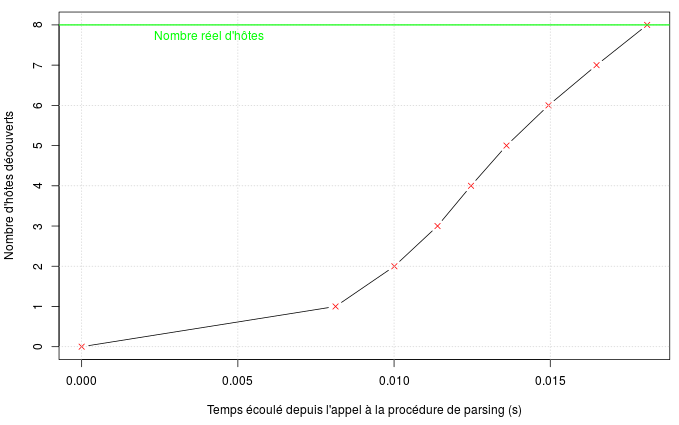
\includegraphics[width=0.7\linewidth]{fpingmean}
     \caption{Moyenne des mesures des temps de découverte pour \texttt{fping}}
     \label{fpingmean}
\end{figure}

\vspace{0.1cm}

On observe que la découverte complète du réseau se fait très rapidement (18 ms en moyenne), en un seul premier appel à la fonction de parsing qui trouve dans la sortie du programme l'information relative à la totalité des hôtes du réseau. Cela a donc pris au total un peu plus de 10 secondes pour trouver les 8 hôtes. La plage IP donnée en paramètre au Module est 192.168.56.3-255, le serveur DHCP de Virtualbox en mode ``réseau privé hôte" distribuant les adresses dans cette zone (les deux premières adresses sont réservées au serveur DHCP et à la machine hôte). Le programme \textit{fping} parcourt cette plage séquentiellement, en partant des plus petites adresses. Les adresses allouées aux hôtes virtuels sont les 8 plus hautes de sorte à se placer dans le pire des cas. En conjugaison avec le fait que le masque d'un réseau domestique est souvent de 24 bits comme considéré ici, les expériences menées reproduisent au mieux la réalité et s'avèrent concluantes.\\ 

 \par À noter que les autres paramètres du Module influent sur ces mesures : si le paramètre \texttt{period} qui désigne le temps en millisecondes entre une retentative sur un même hôte avait été mis à une valeur supérieure à celle par défaut de 3 secondes, tous les hôtes n'auraient peut être pas étés découverts à la première lecture 10 secondes après le lancement. Effectivement, à la lecture du pipe recueillant la sortie du programme, certaines lignes peuvent être tronquées et non parsables (celles du début et de la fin du texte lu). Cependant, la valeur par défaut de 3 secondes et celle de l'intervalle entre deux lectures permettent d'éviter cela par la redondance d'information, ainsi que des précautions prises dans l'implémentation même.\\


\minit{Mesures pour \texttt{nmapexplo}}
\vspace{0.1cm}

\par Le Module \texttt{nmap} étant actif, ce n'est pas une lecture de la sortie du programme en cours qui est faite à intervalles réguliers mais bien un nouvel appel et une exécution du programme \textit{nmap} dont la sortie est parsée une fois sa terminaison. On ne tient donc pas compte du timer d'expiration entre chaque exécution : le temps de référence est le premier appel à la fonction \textit{launch()} du Module. Les mesures se terminent quand les 8 hôtes sont découverts après le parsing d'une de ces exécutions. Le graphique obtenu est donné par la \wordlink{explomean}{figure} (également une moyenne des temps sur 5 expérimentations).\\

\begin{figure}[!ht]
\centering
     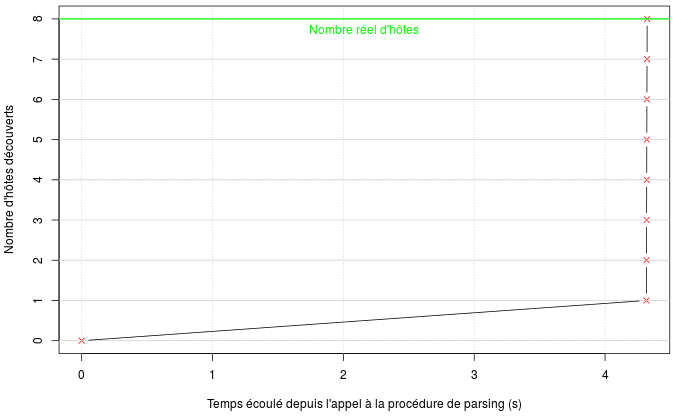
\includegraphics[width=0.75\linewidth]{explomean}
     \caption{Moyenne des mesures des temps de découverte pour \texttt{nmapexplo}}
     \label{explomean}
\end{figure}

\vspace{0.1cm}

\par Comme dans le cas de \texttt{fping}, \texttt{nmapexplo} trouve les 8 hôtes d'une seule fois (dés la première exécution ici), et ce pour chacune des 5 exécutions. On observe que nmap s'est exécuté pendant 4.3 secondes en moyenne à la suite de quoi la fonction de parsing a été appelée. Les 8 hôtes sont alors instanciés dans l'application en 10 ms en moyenne. Les moyennes sont représentatives, les variance associées ne s'élevant pas au dessus de 0.35 secondes.\\

\par La configuration du réseau est identique (plage IP, hôtes aux adresses les plus hautes). L'ordre de balayage n'a ici pas d'importance : les résultats pour le réseau entier passé en paramètre sont retournés d'un bloc à la fin de l'exécution de \textit{nmap}, ce qui prend ici un peu plus de 4 secondes pour les 252 adresses considérées. Bien que par nature le Module \texttt{nmapexplo} soit moins réactif aux changements du réseau (cela dépend de l'intervalle de temps auquel il s'exécute), il a l'avantage par rapport à \texttt{fping} de renseigner d'autres informations telles que l'adresse MAC, potentiellement le nom d'hôte et le fabriquant.

\newpage

\subsection{Application dans un environnement domestique}

Avant de lancer la Routine de surveillance contenant les Modules de découverte et récolte d'informations sur les hôtes, l'état du réseau est consulté via l'interface web du modem. En comptant le modem lui-même, 8 hôtes sont dénombrés comme actifs sur le réseau dont 7 connus. Un schéma récapitulatif de la composition du réseau, tel qu'il est connu, est donné par la \wordlink{mynetwork}{figure}. Tous ces appareils se sont vus allouer une adresse IPv4 par l'unique modem/routeur de l'habitation dans la plage 192.168.1.2-63.\\

\begin{figure}[!ht]
\centering
     \includegraphics[width=0.75\linewidth]{mynetwork}
     \caption{Composition du réseau domestique à analyser}
     \label{mynetwork}
\end{figure}

\vspace{0.1cm}

\par La Routine est configurée comme indiqué par la \wordlink{routinedisc}{figure}, avec les Modules et leurs paramètres par défaut :\\
\begin{itemize}
\item[$\bullet$] \texttt{fping} : à l'aide de requêtes ICMP, détermine l'IP des hôtes peuplant le réseau et régule leur état (connecté ou non) en opérant une lecture de la sortie du programme en cours toutes les 10 secondes
\vspace{0.1cm}
\item[$\bullet$] \texttt{nmapexplo} : balaie le réseau à intervalle de 20 secondes, découvrant les hôtes et leurs caractéristiques en utilisant des techniques de sondes plus évoluées que par ICMP
\vspace{0.1cm}
\item[$\bullet$] \texttt{nmapports} : découvre les ports ouverts d'un hôte (teste par défaut les 50 ports les plus utilisés généralement). Cette inspection des ports se révèle beaucoup plus coûteuse en temps (de facto en ressources), ce Module s'exécutera donc plus rarement que la simple exploration du réseau (240 secondes)

\end{itemize}

\vspace{0.2cm}

\begin{figure}[!ht]
\centering
     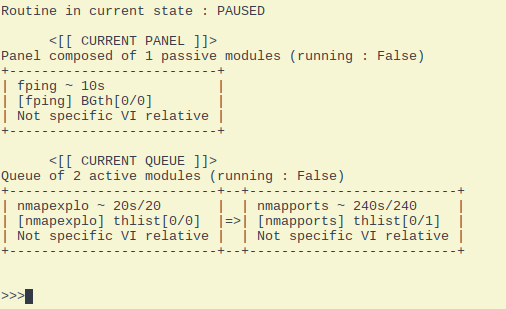
\includegraphics[width=0.6\linewidth]{routineDisc}
     \caption{Configuration d'une Routine pour découvrir les hôtes du réseau domestique}
     \label{routinedisc}
\end{figure}

\vspace{0.3cm}

\newpage

\par Une fois la configuration terminée, la Routine est lancée et son état est passé à ``en cours". Le Module \texttt{fping} lance le programme associé et les hôtes trouvés sont instanciés comme des Instances Virtuelles dans la Netmap dès la première lecture, soit 10 secondes après le lancement de la Routine. Seule leur IP est renseignée, mais d'autres informations sont ajoutées dès la terminaison de l'exécution de \texttt{nmapexplo} un peu plus de 10 secondes plus tard (comprend l'exécution de \textit{nmap}). À ce stade, les 8 équipements sont déjà référencés dans la Netmap avec assez d'information pour les identifier formellement : adresses IP et MAC, nom d'hôte et fabricant présumé pour certains. Une ligne temporelle illustrant les cycles de la Routine ainsi que la vue d'ensemble de la Netmap obtenue sont illustrées par les \wordlink{timeline}{figures} et \wordlink{netmapdisc}{}.

\begin{figure}[!ht]
\centering
     \includegraphics[width=\linewidth]{timeline}
     \caption{Cycles d'exécutions des Modules dans la Routine établie}
     \label{timeline}
\end{figure}

\vspace{0.3cm}

\begin{figure}[!ht]
\centering
     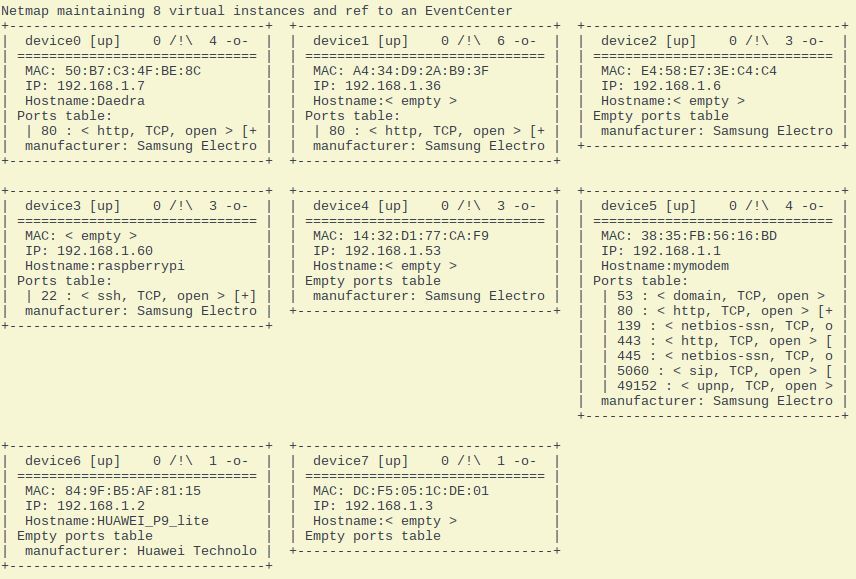
\includegraphics[width=0.9\linewidth]{netmapDisc}
     \caption{État de la Netmap après 5 minutes de travail autonome de la Routine}
     \label{netmapdisc}
\end{figure}

\vspace{0.2cm}

On observe que toutes les adresses IP allouées dans le réseau ont été correctement restituées dans l'application, associant chacune à une Instance Virtuelle différente. Il en va de même pour les adresses MAC, excepté pour la carte Raspberry. Effectivement, dans les résultats de son scan, \textit{nmap} les renseigne toutes sauf celle de l'hôte depuis lequel il a été lancé. Ce n'est pas modifiable nativement, mais considéré comme acceptable car ce n'est théoriquement pas cet hôte que l'utilisateur désire surveiller. Les noms d'hôtes ont été trouvés pour 4 des 8 appareils. Les fabricants sont devinés par \textit{nmap} en se basant sur le préfixe de l'adresse MAC et de sa base de données interne. Il s'agit donc dans certain cas uniquement du fabricant de la carte réseau des hôtes. Les ports découverts affichés sont ceux réellement ouverts et dont \textit{nmap} est confiant vis-à-vis du service associé (corrélé à un niveau allant de 3 à 10). La détection du réseau semble donc assez efficace que pour s'en faire une représentation précise après 5 minutes d'activité de la Routine.

\newpage

\par Par défaut \texttt{nmapports} va, pour chaque hôte, tester le statut des 50 ports les plus utilisés généralement. Après quelques minutes d'activité, la Routine de surveillance aura fait converger la Netmap vers l'état actuel du réseau. Chaque Instance Virtuelle est consultable individuellement, mais les informations principales sont résumées dans la vue d'ensemble donnée par la \wordlink{netmapdisc}{figure}. Afin d'en découvrir davantage, le paramètre \texttt{version} de l'instance de \texttt{nmapports} dans la Routine est passé à vrai. Cela rallonge son temps d'exécution (de 35 secondes à plus de 2 minutes pour un sous-réseau de masque /24) mais permet d'obtenir des informations à propos de la version des services actifs sur les ports, ainsi que le système d'exploitation et le hardware. Ces informations sont retournées par \textit{nmap} en utilisant le format standardisé CPE (Common Platform Enumeration\footnote{\url{https://nmap.org/book/output-formats-cpe.html}}). La \wordlink{modemdisc}{figure} illustre les résultats obtenus pour l'Instance Virtuelle correspondant au modem après une nouvelle exécution de \texttt{nmapports}, détaillant les services devinés sur ses ports ouverts.

\vspace{0.1cm}

\begin{figure}[!ht]
\centering
     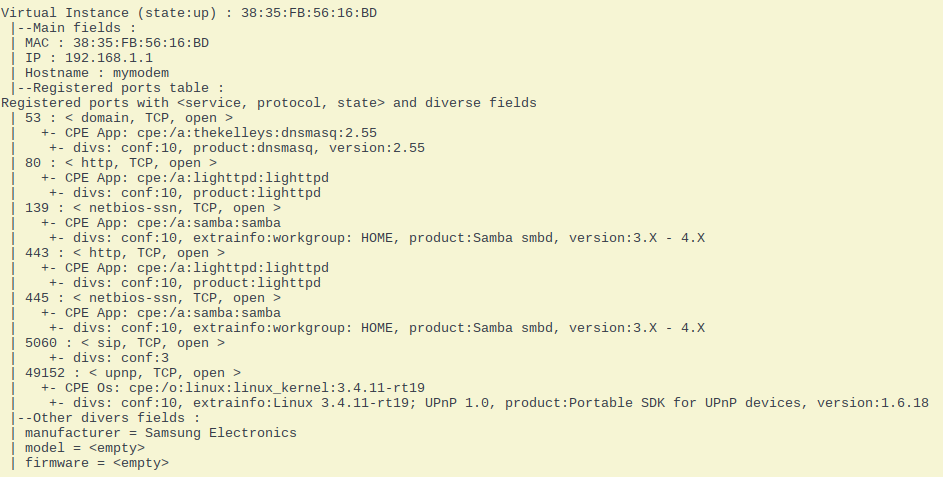
\includegraphics[width=\linewidth]{modemDisc}
     \caption{Affichage détaillé des informations récoltées pour le modem}
     \label{modemdisc}
\end{figure}


\newpage

\subsection{Évaluation de la détection de menaces}

À l'heure actuelle, un seul Module est complètement opérationnel dans la découverte de vulnérabilité : \texttt{nmapvulners}. Il s'agit d'un Module actif basé sur le script \textit{nmap-vulners}, intégrable à une exécution de \textit{nmap} grâce au Nmap Script Engine. Pour chaque hôte découvert lors du balayage, le script va faire en sorte de deviner la version des services actifs sur les ports ouverts. Si cela est possible, une requête est alors effectuée en ligne vers la base de données Vulners. Si une entrée CVE correspond à la version du service recherché, une menace est instanciée dans l'application et remontée jusqu'à l'utilisateur. Afin d'obtenir plus de détail sur la vulnérabilité du service tournant sur l'un de ses appareils, un lien internet vers le descriptif CVE (dans Vulners) est fourni à l'utilisateur.

\subsubsection{Simulation d'équipement virtuel vulnérable}

L'objectif est de vérifier qu'en installant intentionnellement un logiciel vulnérable sur une machine virtuelle (une des Debian Stretch utilisée pour les tests précédents), l'application le détecte et en alerte l'utilisateur. La procédure employée est la suivante :

\begin{enumerate}
\item Recherche dans la base de données Vulners une entrée de type CVE (\url{https://vulners.com/search?query=type:cve}) pour un logiciel orienté serveur dont une faille a été rendue publique
\vspace{0.1cm}
\item Rechercher les sources correspondant à une version indiquée comme vulnérable dans le descriptif CVE, installer le programme obsolète sur la machine virtuelle
\vspace{0.1cm}
\item Mettre en route le service qui écoutera sur son port par défaut et tester la bonne détection de ce service par \textit{nmap}
\vspace{0.1cm}
\item Dans l'application, instancier le Module \texttt{nmapvulners} avec si nécessaire des paramètres adaptés (port peu commun, ...) et lancer son exécution
\vspace{0.1cm}
\item Vérifier que la menace est bien détectée et l'alerte donnée à l'utilisateur, pointant vers les bons descriptifs CVE initialement considérés
\end{enumerate}

Les logiciels alors considérés sont les suivants :

\begin{itemize}
\item[$\bullet$] \textit{proftpd}, version 1.3.4 (2 CVEs\footnote{\url{https://vulners.com/search?query=affectedSoftware.name:proftpd AND type:cve AND affectedSoftware.version:1.3.4}})
\item[$\bullet$] \textit{lighttpd}, version 1.4.42 (1 CVE\footnote{\url{https://vulners.com/search?query=affectedSoftware.name:lighttpd AND type:cve AND affectedSoftware.version:1.4.42}})
\end{itemize}
~\\

\par Après avoir instancié le Module \texttt{nmapvulners}, le scann est lancé sur la machine ciblée. On observe que des vulnérabilités ont en effet été découvertes, et si une adresse mail avait été fournie alors un récapitulatif similaire à ce qui est affiché dans l'application (\wordlink{threatsvm}{figure}) est envoyé. À chaque menace un niveau de dangerosité est associé, allant de 1 à 10. Dans le cas de \texttt{nmapvulners}, il s'agit du CVSS (Common Vulnerability Scoring System\footnote{\url{https://fr.wikipedia.org/wiki/Common_Vulnerability_Scoring_System}}).

\vspace{0.1cm}

\begin{figure}[!ht]
\centering
     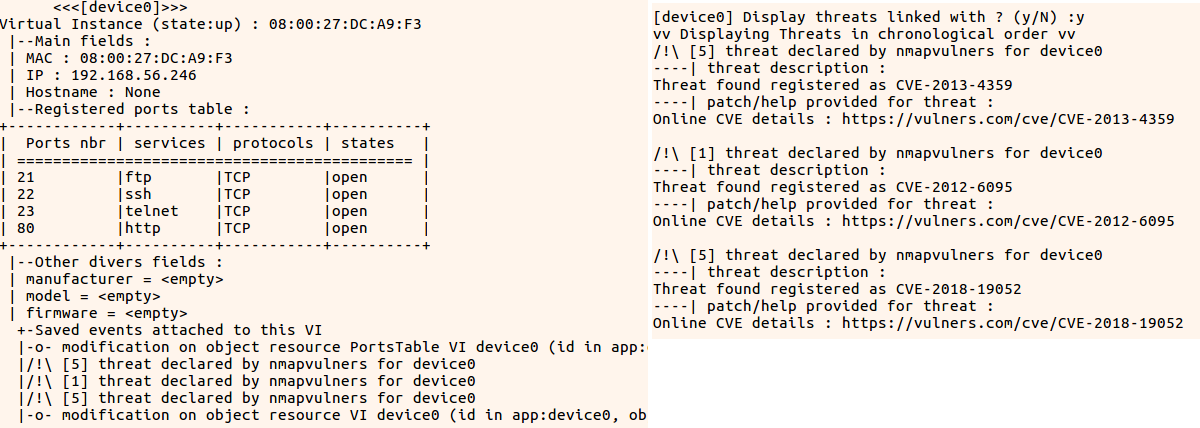
\includegraphics[width=1.05\linewidth]{threatsVM}
     \caption{Résultat d'une exécution de \texttt{nmapvulners} (vulnérabilités trouvées)}
     \label{threatsvm}
\end{figure}

\newpage

En suivant le lien donné pour chaque menace, on retrouve bien les CVEs attendues. Cependant, le Module n'est pas du tout exhaustif. Si on s'en réfère à une recherche manuelle dans la base de données Vulners sans spécifier de version pour \textit{proftpd}, on tombe sur 36 résultats au lieu des 2 initiaux. Certains sont bien pertinents, décrivant une vulnérabilité dont version la 1.3.4 de \textit{proftp} n'est pas exempte. Cela est dû au fait que certaines entrées dans la base de données ne renseignent pas formellement les versions affectées, mais uniquement dans une description textuelle. Ces entrées ne se retrouvent donc pas dans les résultats d'une recherche pour une version spécifique.\\

\par De plus, \texttt{nmapexplo} peut tout simplement échouer à deviner la version ou le service associé à un port. Par exemple, malgré le fait que \textit{telnet} soit un programme sujet à des failles (4 CVEs sont renseignées sur Vulners), \textit{nmap} ne parvient à deviner que l'activité de \textit{telnet} sur le port 23 sans information complémentaire sur sa version. En conséquence, aucune requête n'est faite par le script vers l'API de Vulners. Il arrive également que \textit{nmap} ne reconnaisse pas le protocole, comme par exemple en testant le programme serveur Mosquitto dans le cadre du protocole MQTT (utilisé dans l'IoT, cf. \wordlink{IoT_prot}{sous-section}).

\subsubsection{Utilisation dans un réseau domestique peuplé}

Le réseau utilisé est celui présenté pour les tests de découverte des hôtes (\wordlink{mynetwork}{figure}), reproduit au mieux. La Routine utilisée n'est remplie que des Modules \texttt{fping} et \texttt{nmapports}. Pour ce dernier, afin de couvrir un nombre de services plus larges, le paramètre \texttt{top-ports} est mis à 30 de sorte que \textit{nmap} inspecte les 30 ports les plus utilisés généralement pour chaque hôte. Le temps d'exécution est alors de 30 secondes pour le sous-réseau /24 considéré. La \wordlink{realvulns}{figure} illustre la vue générale de la Netmap après 5 minutes d'activité de la Routine. 

\begin{figure}[!ht]
\centering
     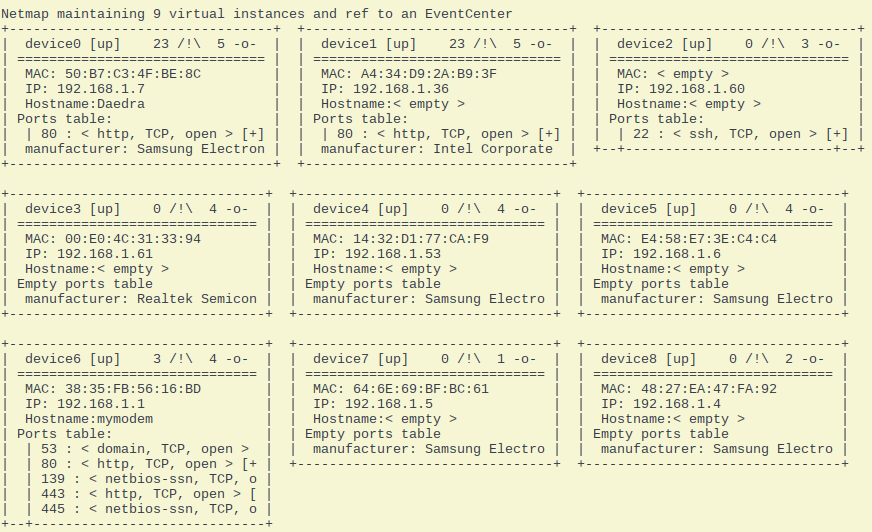
\includegraphics[width=1\linewidth]{netmapvulns}
     \caption{Vue d'ensemble du réseau domestique est des menaces trouvées (/!\textbackslash)}
     \label{realvulns}
\end{figure}

\par Des menaces ont été détectées pour 3 appareils, 2 d'entre eux étant des ordinateurs desktop et le troisième le modem lui-même. Pour les ordinateurs, il s'agit de vulnérabilités liées au service web \textit{Apache} qui avait été installé à la même époque sur les deux machines. Depuis, 23 CVEs ont visiblement été déclarées pour ces versions obsolètes. En ce qui concerne le modem, il s'agit du service de DNS interne (port 53) dont la version est sujette à 3 CVEs. Les autres appareils semblent plus protégés, mais il est nécessaire de garder à l'esprit que seuls 30 des ports les plus répandus ont été analysés pour fluidifier le balayage complet du réseau. Un ciblage plus spécifique sur quelques hôtes avec plus de ports, ou des ports plus pertinents connaissant l'appareil, peut aisément être réalisé par reconfiguration du Module ou en en créant une nouvelle instance.

\newpage

\section{Conclusion}

\par La première partie de ce projet a été l'occasion de se plonger dans ce que la littérature proposait en terme de cybersécurité pour les foyers. Beaucoup de thèmes ont étés abordés en surface car l'application à réaliser n'était pas fixée. Aussi, une vue globale était nécessaire pour décider quels seraient les tenants et les aboutissants de la partie implémentation.\\

\par Pour cette application, le soin apporté à l'intégration générique de n'importe quel programme arbitraire est un investissement sur le long terme. À l'heure actuelle, le nombre de module disponibles est restreint par manque de temps non pas pour leur implémentation, mais pour la recherche et les expérimentations nécessaires avant l'intégration. Effectivement, la seule difficulté est inhérente au fait qu'il est nécessaire de traduire les sorties de chaque programme spécifique. Outre cela, beaucoup d'améliorations sont encore facilement apportables à l'application : interface graphique, gestion des dépendances, etc.

\newpage

\bibliographystyle{plain}
\bibliography{articles}

\end{document}